\documentclass{beamer}

\usepackage{tikz}
\usepackage{pgfplots}
\usepackage{amsmath}
\usepackage{xcolor}
\usepackage{booktabs}
\usepackage{colortbl}
\usepackage{array}

\pgfplotsset{compat=newest}

% Minimal, no headers/footers/nav symbols
\mode<presentation>{
  \usetheme{default}
  \setbeamertemplate{navigation symbols}{}
  \setbeamertemplate{headline}{}
  \setbeamertemplate{footline}{}
}


% Custom colors
\definecolor{myblue}{RGB}{39,64,139}
\definecolor{homecolor}{RGB}{0,102,204}
\definecolor{foreigncolor}{RGB}{204,51,0}
\definecolor{capitalcolor}{RGB}{0,102,204}    % or whatever blue you use
\definecolor{laborcolor}{RGB}{204,51,0}        % or match foreigncolor

% SELECTIVE COMPILATION:
\newcommand{\showanswers}{1}  % 0 = hide, 1 = show

% Pattern example for selection compilation
% \ifnum\showanswers=1
% \section{Answers}
% Content here...
% \fi


\begin{document}


\section{International Economics Course}

\ifnum\showanswers=0
\subsection{Ricardian Trade with Answers}

\subsubsection{Introduction to Ricarian Trade}

%========================
% Slide 1: Title Slide
%========================

\begin{frame}

\vspace{1.5cm}

\centering
{\Large \textbf{Tutorial 1: Labor Productivity and Comparative Advantage}} \\[0.5cm]
{\large The Ricardian Model} \\[1.0cm]

{\small 7QQMM209: International Economics} \\[0.3cm]
{\small King's College London}

\vfill

\end{frame}

\begin{frame}{Tutorial: Objectives \& mode of operation}

\begin{itemize}
    \item Objectives
        \begin{itemize}
            \item Ensure \& improve understanding of textbook content
            \item Discuss models' underlying assumptions \& implications \\~\\
        \end{itemize}
    
    \item Mode of operation
        \begin{itemize}
            \item Reason through the numerical \& visual examples from the textbook (KOM)
            \item Guided work interchangeably in small groups \& among all
            \item Learning from mutual exchange
            \item Open discussion with respect for different backgrounds \\~\\
        \end{itemize}

    \item To Do's
    \begin{itemize}
        \item Before class: Reason through slides \& try answer questions
        \item During class: Discuss in small groups, share responses with all
        \item Before exam: Go through questions \& model solutions
    \end{itemize}
    
        
\end{itemize}    
\end{frame}

%========================
% Slide 2: Overview - Key Messages
%========================

\begin{frame}{Overview: Why Do Countries Trade?}

\textbf{Two fundamental motivations for international trade:}

\begin{enumerate}
    \item \textbf{Economies of scale} --- Countries benefit from specialization because it allows larger-scale, more efficient production \\[0.5cm]
    
    \item \textbf{Comparative advantage} --- Countries differ in their ability to produce goods, so they can benefit by each producing what they do \textit{relatively} better
\end{enumerate}

\vspace{0.5cm}

\textbf{This week's focus:} The Ricardian model explains trade through \textbf{differences in labor productivity} across countries.

\vspace{0.3cm}

\textit{Key insight:} What matters is \textbf{relative} (comparative) advantage, not \textbf{absolute} advantage.

\end{frame}
\begin{frame}{Can someone explain the different assumptions about return to scale \& and how they relate to trade?}

\begin{itemize}
    \item Constant returns to scale \\~\\
    \item Increasing returns to scale \\~\\
    \item Decreasing returns to scale
\end{itemize}
\end{frame}


%========================
% Slide 3: Key Concepts Covered
%========================

% \begin{itemize}
%     \item \textbf{Absolute vs. Comparative Advantage}
%     \begin{itemize}
%         \item Absolute: Who can produce more with same resources?
%         \item Comparative: Who has the lower \textit{opportunity cost}?
%     \end{itemize}
    
%     \vspace{0.3cm}
    
%     \item \textbf{Opportunity Cost}
%     \begin{itemize}
%         \item What must be given up to produce one more unit?
%         \item Measured by the ratio of unit labor requirements
%     \end{itemize}

\begin{frame}{Key Concepts for this tutorial}

\begin{itemize}
    \item Absolute vs. Comparative Advantage \\~\\ 
    \item Opportunity Cost \\~\\
    \item Production \& Consumption Possibility Frontiers (PPF) \\~\\
    \item Partial \& General Equilibrium \\~\\
    \item Relative Supply (RS) \& Relative Demand (RD) \\~\\
    \item Gains from Trade (How trade expands consumption possibilities)
\end{itemize}

\end{frame}



%========================
% Slide 10: Historical Context - Trade Models Timeline
%========================

\begin{frame}{Where Does Ricardo Fit? A Historical Overview}

\textbf{Evolution of Trade Theory:}

\vspace{0.3cm}

\begin{tabular}{lp{7cm}}
\textbf{1776} & \textbf{Adam Smith:} Absolute advantage \\[0.2cm]
\textbf{1817} & \textbf{David Ricardo:} Comparative advantage based on \textit{labor productivity differences} \\[0.2cm]
\textbf{1930s} & \textbf{Heckscher-Ohlin:} Comparative advantage based on \textit{factor endowments} (capital, land, labor) \\[0.2cm]
\textbf{1970s+} & \textbf{New Trade Theory:} Economies of scale, product differentiation, intra-industry trade \\[0.2cm]
\textbf{2000s+} & \textbf{New New Trade Theory:} Firm heterogeneity
\end{tabular}

\vspace{0.5cm}

\textit{Ricardo's contribution:} Showed that even if a country is less productive in \textbf{all} goods, it can still gain from trade by specializing in what it does \textbf{relatively} better.

\end{frame}

%========================
% Slide 4: Key Ingredients of the Ricardian Model
%========================

\begin{frame}{The Ricardian Model: Key Ingredients}
\vspace{-0.5cm}

\textbf{Two-Good, Two-Country Model:}

\vspace{0.5cm}

\begin{columns}[T]
\begin{column}{0.48\textwidth}
\textbf{Home Country}
\vspace{0.25cm}
\begin{itemize}
    \item Labor force: $L$ \\~\\
    \item Unit labor requirement:
    \begin{itemize}
        \item Cheese: $a_{LC}$ hours/lb
        \item Wine: $a_{LW}$ hours/gal
    \end{itemize}
\end{itemize}
\end{column}

\begin{column}{0.48\textwidth}
\textbf{Foreign Country}
\vspace{0.25cm}
\begin{itemize}
    \item Labor force: $L^*$ \\~\\
    \item Unit labor requirement:
    \begin{itemize}
        \item Cheese: $a^*_{LC}$ hours/lb
        \item Wine: $a^*_{LW}$ hours/gal
    \end{itemize}
\end{itemize}
\end{column}
\end{columns}

\vspace{0.5cm}

\textbf{Production Constraint (Home):}
$$a_{LC} \cdot Q_C + a_{LW} \cdot Q_W \leq L$$

\end{frame}




% \begin{frame}{Where can you see productivity in they key ingredients of the Ricardian model?}
% \end{frame}

%========================
% Where can you see productivity? - Answer slide with progressive reveal
%========================

\begin{frame}{Where can you see productivity in the key ingredients of the Ricardian model?}

\onslide<2->{
\vspace{0.3cm}
\textbf{Productivity appears in the unit labor requirements ($a_{Li}$):}

\begin{itemize}
    \item $a_{Li}$ = hours needed to produce 1 unit of good $i$
    \item Productivity = $\frac{1}{a_{Li}}$ = output per hour
    \item \textbf{Lower} unit labor requirement = \textbf{higher} productivity
\end{itemize}
}

\vspace{0.3cm}

\onslide<3->{
\textbf{Example (Cheese):}

\vspace{0.1cm}

\begin{center}
\begin{tabular}{lcc}
\toprule
& \textbf{Home} & \textbf{Foreign} \\
\midrule
Unit labor req. ($a_{LC}$) & 1 hour/lb & 6 hours/lb \\
Productivity ($\frac{1}{a_{LC}}$) & 1 lb/hour & $\frac{1}{6}$ lb/hour \\
\bottomrule
\end{tabular}
\end{center}

\vspace{0.3cm}

Home is \textbf{6 times more productive} in cheese production.

\vspace{0.2cm}

\small{\textit{Similarly for wine: Home needs 2 hrs/gal vs Foreign's 3 hrs/gal $\Rightarrow$ Home is 1.5 times more productive.}}
}

\end{frame}

%========================
% Slide 7: Key Assumptions
%========================

\begin{frame}{Key Assumptions of the Ricardian Model}

\begin{enumerate}
    \item \textbf{One factor of production:} Labor only
    
    \vspace{0.2cm}
    
    \item \textbf{Constant returns to scale:} Unit labor requirements are fixed
    
    \vspace{0.2cm}
    
    \item \textbf{Perfect labor mobility within countries:} Workers can move freely between sectors $\Rightarrow$ single wage rate
    
    \vspace{0.2cm}
    
    \item \textbf{Perfect competition:} Price = Cost of production
    
    \vspace{0.2cm}
    
    \item \textbf{Full employment:} All labor is used
    
    \vspace{0.2cm}
    
    \item \textbf{No transport costs or trade barriers} (initially)
    
    \vspace{0.2cm}
    
    \item \textbf{Labor immobile between countries}
\end{enumerate}

\vspace{0.3cm}

\textit{Implication:} In absence of trade, relative prices = relative unit labor requirements

$$\frac{P_C}{P_W} = \frac{a_{LC}}{a_{LW}}$$

\end{frame}


%========================
% SECTION: Visual & Numerical Exercises
% India-Thailand Rice and Cloth Example
%========================

\subsubsection{Visual \& Numerical Exercises}

%========================
% Setup Slide: The Numerical Case
%========================

\begin{frame}{Numerical Example: India and Thailand}

\textbf{Setup:} Two countries, two goods, one factor (labor)

\vspace{0.1cm}

\begin{center}
\begin{tabular}{lcc}
\toprule
& \textbf{India} & \textbf{Thailand} \\
\midrule
Output per hour: Rice (kg) & 10 & 5 \\
Output per hour: Cloth (meters) & 5 & 2 \\
\midrule
Labor force (hours) & 1,000 & 500 \\
\bottomrule
\end{tabular}
\end{center}

\vspace{0.3cm}

\textit{Note:} Output per hour = Labor productivity = $\frac{1}{a_L}$ (inverse of unit labor requirement)

\vspace{0.3cm}

\textbf{Equivalent unit labor requirements:}

\begin{center}
\begin{tabular}{lcc}
\toprule
& \textbf{India} & \textbf{Thailand} \\
\midrule
$a_{LR}$ (hours per kg of rice) & $\frac{1}{10} = 0.1$ & $\frac{1}{5} = 0.2$ \\
$a_{LC}$ (hours per meter of cloth) & $\frac{1}{5} = 0.2$ & $\frac{1}{2} = 0.5$ \\
\bottomrule
\end{tabular}
\end{center}

\end{frame}

%========================
% Question 1: Absolute Comparative Advantage
%========================

\begin{frame}{Question 1: Absolute Advantage}

\textbf{a) Write a definition of absolute comparative advantage in your own words.}

\vspace{1cm}

\textbf{b) Show numerically which country has absolute advantage in each good.}

\end{frame}

%------------------------
% Question 1: Answer
%------------------------
\begin{frame}{Question 1: Answer}

\textbf{a) Definition of absolute advantage:}

\vspace{0.2cm}

A country has \textbf{absolute advantage} in producing a good if it can produce \textit{more output per unit of input} (higher productivity) than another country --- equivalently, if it requires \textit{fewer inputs per unit of output} (lower unit labor requirement).

\vspace{0.2cm}

\textbf{b) Numerical demonstration:}
\vspace{-0.2cm}
\begin{center}
\small
\begin{tabular}{lcccc}
\toprule
& \textbf{India} & \textbf{Thailand} & \textbf{Comparison} & \textbf{Abs. Adv.} \\
\midrule
\multicolumn{5}{l}{\textit{Productivity (output/hour):}} \\
Rice (kg/hour) & 10 & 5 & $10 > 5$ & \textcolor{homecolor}{\textbf{India}} \\
Cloth (m/hour) & 5 & 2 & $5 > 2$ & \textcolor{homecolor}{\textbf{India}} \\
\midrule
\multicolumn{5}{l}{\textit{Unit labor requirement (hours/unit):}} \\
Rice (hours/kg) & 0.1 & 0.2 & $0.1 < 0.2$ & \textcolor{homecolor}{\textbf{India}} \\
Cloth (hours/m) & 0.2 & 0.5 & $0.2 < 0.5$ & \textcolor{homecolor}{\textbf{India}} \\
\bottomrule
\end{tabular}
\end{center}

\vspace{0.2cm}

\textbf{Conclusion:} India has absolute advantage in \textbf{both} goods. But does this mean Thailand cannot gain from trade?

\end{frame}

%========================
% Question 2: Relative/Comparative Advantage
%========================

\begin{frame}{Question 2: Comparative Advantage \& Opportunity Costs}

\textbf{a) Write a definition of relative comparative advantage in your own words.}

\vspace{0.5cm}

\textbf{b) Show numerically which country has comparative advantage in each good using opportunity costs.}

\end{frame}

%------------------------
% Question 2: Answer
%------------------------

\begin{frame}{Question 2: Answer}

\textbf{a) Definition of comparative advantage:}

A country has \textbf{comparative advantage} in producing a good if its \textit{opportunity cost} of producing that good is lower than in another country.

\vspace{0.3cm}

\textbf{b) Calculating RCA/opportunity costs:}

\vspace{0.2cm}

\textbf{Opportunity cost of 1 meter of cloth (in kg of rice):}
\begin{itemize}
    \item \textcolor{homecolor}{India:} $\frac{\text{Rice output/hour}}{\text{Cloth output/hour}} = \frac{10}{5} = 2$ kg of rice
    \item \textcolor{foreigncolor}{Thailand:} $\frac{5}{2} = 2.5$ kg of rice
\end{itemize}

\vspace{0.2cm}

\textbf{Opportunity cost of 1 kg of rice (in meters of cloth):}
\begin{itemize}
    \item \textcolor{homecolor}{India:} $\frac{5}{10} = 0.5$ meters of cloth
    \item \textcolor{foreigncolor}{Thailand:} $\frac{2}{5} = 0.4$ meters of cloth
\end{itemize}

\vspace{0.3cm}

\textbf{Comparative advantage:}
\begin{itemize}
    \item \textcolor{homecolor}{India}: Lower OC in \textbf{cloth} (2 < 2.5) $\Rightarrow$ CA in cloth
    \item \textcolor{foreigncolor}{Thailand}: Lower OC in \textbf{rice} (0.4 < 0.5) $\Rightarrow$ CA in rice
\end{itemize}

\end{frame}

%========================
% Question 3: Empirical Validation Problem
%========================

\begin{frame}{Question 3: The Empirical Validation Problem}

\textbf{Assuming countries fully specialize in the activity for which they have comparative advantage, what problem arises for empirical validation of Ricardo's theory?}

\end{frame}

%------------------------
% Question 3: Answer
%------------------------

\begin{frame}{Question 3: Answer}

\textbf{The empirical validation problem:}

\vspace{0.3cm}

If countries \textbf{fully specialize}:
\begin{itemize}
    \item India produces \textit{only} cloth
    \item Thailand produces \textit{only} rice
\end{itemize}

\vspace{0.3cm}

\textbf{Problem:} We cannot observe what India's rice productivity \textit{would have been} or Thailand's cloth productivity \textit{would have been}.

\vspace{0.3cm}

$\Rightarrow$ \textbf{No data exists} for the good a country does not produce!

\vspace{0.5cm}

\textbf{Implications for testing the theory:}
\begin{itemize}
    \item Cannot directly compare unit labor requirements across countries for goods not produced
    \item Must use indirect methods (e.g., Balassa's revealed comparative advantage, or pre-trade data)
    \item The theory predicts complete specialization, but we observe incomplete specialization in reality
\end{itemize}

\end{frame}


%========================
% Question 4: Production Possibility Frontier - UPDATED
% Using Q notation, F/P labels, dual calculation methods
%========================

\begin{frame}{Question 4: Drawing the Production Possibility Frontier}

\vspace{-0.2cm}

\textbf{Draw India's and Thailand's Production Possibility Frontier.}

\vspace{0.2cm}

\begin{enumerate}
    \item What is on the x-and y-axis?
    \item How do you determine the intersection between PPF and x-axis, and PPF and y-axis?
    \item How can you numerically calculate the slope?
    \item How can you infer from the slopes which country has relative comparative advantage?
\end{enumerate}

\end{frame}

%------------------------
% Question 4: PPF Step 1 - Axes only
%------------------------

\begin{frame}{Question 4: Step 1 Setting Up The Axes}

\begin{columns}[T]
\begin{column}{0.48\textwidth}
\centering
\textcolor{homecolor}{\textbf{India}} (L = 1,000 hours)

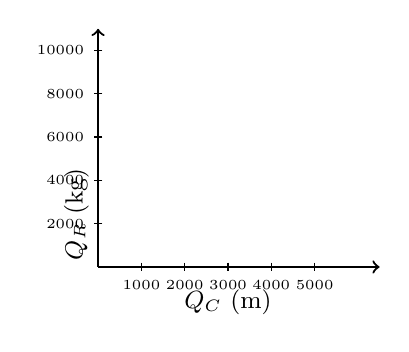
\begin{tikzpicture}[scale=0.55]
    % Axes
    \draw[->, thick] (0,0) -- (6.5,0);
    \draw[->, thick] (0,0) -- (0,5.5);
    
    % Axis labels
    \node[below] at (3,-0.3) {\small $Q_C$ (m)};
    \node[left, rotate=90] at (-0.5,2.5) {\small $Q_R$ (kg)};
    
    % Tick marks and numbers
    \foreach \x in {1,2,3,4,5} {
        \draw (\x,0.1) -- (\x,-0.1);
        \pgfmathsetmacro{\val}{int(\x*1000)}
        \node[below, font=\tiny] at (\x,-0.1) {\val};
    }
    \foreach \y in {1,2,3,4,5} {
        \draw (0.1,\y) -- (-0.1,\y);
        \pgfmathsetmacro{\val}{int(\y*2000)}
        \node[left, font=\tiny] at (-0.1,\y) {\val};
    }
\end{tikzpicture}
\end{column}

\begin{column}{0.48\textwidth}
\centering
\textcolor{foreigncolor}{\textbf{Thailand}} (L* = 500 hours)

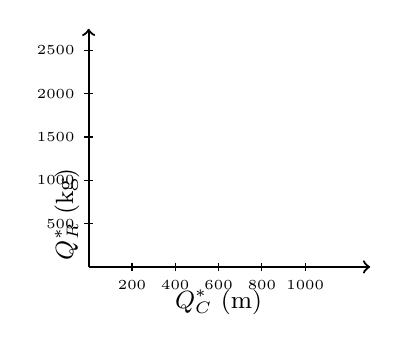
\begin{tikzpicture}[scale=0.55]
    % Axes
    \draw[->, thick] (0,0) -- (6.5,0);
    \draw[->, thick] (0,0) -- (0,5.5);
    
    % Axis labels
    \node[below] at (3,-0.3) {\small $Q^*_C$ (m)};
    \node[left, rotate=90] at (-0.5,2.5) {\small $Q^*_R$ (kg)};
    
    % Tick marks and numbers
    \foreach \x in {1,2,3,4,5} {
        \draw (\x,0.1) -- (\x,-0.1);
        \pgfmathsetmacro{\val}{int(\x*200)}
        \node[below, font=\tiny] at (\x,-0.1) {\val};
    }
    \foreach \y in {1,2,3,4,5} {
        \draw (0.1,\y) -- (-0.1,\y);
        \pgfmathsetmacro{\val}{int(\y*500)}
        \node[left, font=\tiny] at (-0.1,\y) {\val};
    }
\end{tikzpicture}
\end{column}
\end{columns}

\vspace{0.3cm}

\textbf{Question:} What are the maximum quantities each country can produce if it dedicates all labor to one good?

\end{frame}

%------------------------
% Question 4: PPF Step 3 - Intercepts (UPDATED with dual calculation)
%------------------------

\begin{frame}{Question 4: Step 2 Calculating the Intercepts}

\textbf{Intercept = Maximum production if all labor goes to one good}

\vspace{0.2cm}

\textbf{Two equivalent ways to calculate:}

\vspace{-0.1cm}

\begin{center}
\small
$\text{Max output} = L \times \underbrace{\text{(labor productivity)}}_{\text{output per hour}} = \frac{L}{\underbrace{a_{Li}}_{\text{hours per unit}}}$
\end{center}

\vspace{0.3cm}

\begin{columns}[T]
\begin{column}{0.48\textwidth}
\textcolor{homecolor}{\textbf{India}} (L = 1,000)

\small
\textbf{Max Rice:}
\begin{itemize}
    \item $= 1000 \times 10 = $ \textbf{10,000 kg}
    \item $= \frac{1000}{0.1} = $ \textbf{10,000 kg}
\end{itemize}

\textbf{Max Cloth:}
\begin{itemize}
    \item $= 1000 \times 5 = $ \textbf{5,000 m}
    \item $= \frac{1000}{0.2} = $ \textbf{5,000 m}
\end{itemize}
\end{column}

\begin{column}{0.48\textwidth}
\textcolor{foreigncolor}{\textbf{Thailand}} (L* = 500)

\small
\textbf{Max Rice:}
\begin{itemize}
    \item $= 500 \times 5 = $ \textbf{2,500 kg}
    \item $= \frac{500}{0.2} = $ \textbf{2,500 kg}
\end{itemize}

\textbf{Max Cloth:}
\begin{itemize}
    \item $= 500 \times 2 = $ \textbf{1,000 m}
    \item $= \frac{500}{0.5} = $ \textbf{1,000 m}
\end{itemize}
\end{column}
\end{columns}

\end{frame}

%------------------------
% Question 4: PPF Step 4 - Complete PPF with F, P labels and slope
%------------------------

\begin{frame}{Question 4: Step 2 PPF Visualized}

\begin{columns}[T]
\begin{column}{0.48\textwidth}
\centering
\textcolor{homecolor}{\textbf{India}}

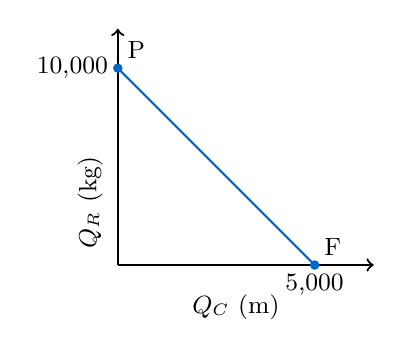
\begin{tikzpicture}[scale=0.5]
    % Axes
    \draw[->, thick] (0,0) -- (6.5,0);
    \draw[->, thick] (0,0) -- (0,6);
    
    % Axis labels
    \node[below] at (3,-0.5) {\small $Q_C$ (m)};
    \node[left, rotate=90] at (-0.7,3) {\small $Q_R$ (kg)};
    
    % PPF line
    \draw[thick, homecolor] (0,5) -- (5,0);
    
    % Intercept labels
    \node[left] at (0,5) {\small 10,000};
    \node[below] at (5,0) {\small 5,000};
    
    % F and P points (India: P at y-intercept, F at x-intercept)
    \filldraw[homecolor] (0,5) circle (3pt);
    \filldraw[homecolor] (5,0) circle (3pt);
    \node[above right, font=\small] at (0,5) {P};
    \node[above right, font=\small] at (5,0) {F};
\end{tikzpicture}
\end{column}

\begin{column}{0.48\textwidth}
\centering
\textcolor{foreigncolor}{\textbf{Thailand}}

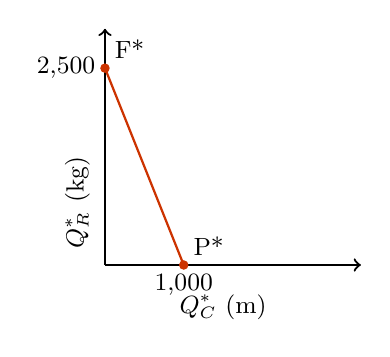
\begin{tikzpicture}[scale=0.5]
    % Axes
    \draw[->, thick] (0,0) -- (6.5,0);
    \draw[->, thick] (0,0) -- (0,6);
    
    % Axis labels
    \node[below] at (3,-0.5) {\small $Q^*_C$ (m)};
    \node[left, rotate=90] at (-0.7,3) {\small $Q^*_R$ (kg)};
    
    % PPF line (steeper)
    \draw[thick, foreigncolor] (0,5) -- (2,0);
    
    % Intercept labels
    \node[left] at (0,5) {\small 2,500};
    \node[below] at (2,0) {\small 1,000};
    
    % F and P points (Thailand: F at y-intercept, P at x-intercept)
    \filldraw[foreigncolor] (0,5) circle (3pt);
    \filldraw[foreigncolor] (2,0) circle (3pt);
    \node[above right, font=\small] at (0,5) {F*};
    \node[above right, font=\small] at (2,0) {P*};
\end{tikzpicture}

\end{column}
\end{columns}

\end{frame}

%------------------------
% Question 4: Explanation of F, P, T notation
%------------------------

\begin{frame}{Question 4: Understanding the F, P, T Notation}

\textbf{What do F, P, and T represent?}

\vspace{0.3cm}

\begin{itemize}
    \item \textbf{P} = \textbf{P}roduction point after specialization
    \begin{itemize}
        \item Where the country produces after trade opens
        \item Each country specializes in its comparative advantage good
    \end{itemize}
    
    \vspace{0.3cm}
    
    \item \textbf{F} = \textbf{F}rontier point (maximum world production)
    \begin{itemize}
        \item The opposite corner of the PPF
        \item Represents full specialization in the \textit{other} good
    \end{itemize}
    
    \vspace{0.3cm}
    
    \item \textbf{T} = \textbf{T}rade consumption point (introduced later)
    \begin{itemize}
        \item Where the country can consume after trading
        \item Lies \textit{beyond} the PPF --- the gains from trade!
    \end{itemize}
\end{itemize}

\vspace{0.3cm}

\small{\textit{Note: India (CA in cloth) has P at rice-max, F at cloth-max; Thailand (CA in rice) has the reverse.}}

\end{frame}


\begin{frame}{Question 4: Step 3 \& 4 Calculating \& interpreting the slope}

\begin{columns}[T]
\begin{column}{0.48\textwidth}
\centering
\textcolor{homecolor}{\textbf{India}}

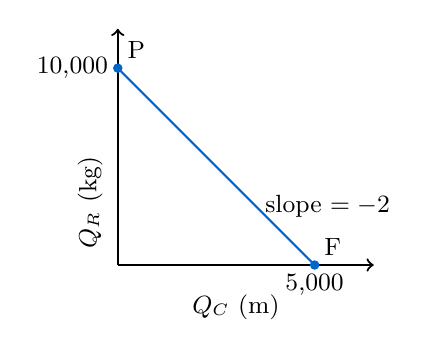
\begin{tikzpicture}[scale=0.5]
    % Axes
    \draw[->, thick] (0,0) -- (6.5,0);
    \draw[->, thick] (0,0) -- (0,6);
    
    % Axis labels
    \node[below] at (3,-0.5) {\small $Q_C$ (m)};
    \node[left, rotate=90] at (-0.7,3) {\small $Q_R$ (kg)};
    
    % PPF line
    \draw[thick, homecolor] (0,5) -- (5,0);
    
    % Intercept labels
    \node[left] at (0,5) {\small 10,000};
    \node[below] at (5,0) {\small 5,000};
    
    % Slope annotation
    \node[right] at (3.5,1.5) {\small slope $= -2$};
    
    % F and P points (India: P at y-intercept, F at x-intercept)
    \filldraw[homecolor] (0,5) circle (3pt);
    \filldraw[homecolor] (5,0) circle (3pt);
    \node[above right, font=\small] at (0,5) {P};
    \node[above right, font=\small] at (5,0) {F};
\end{tikzpicture}

\small{OC of cloth = 2 kg rice}
\end{column}

\begin{column}{0.48\textwidth}
\centering
\textcolor{foreigncolor}{\textbf{Thailand}}

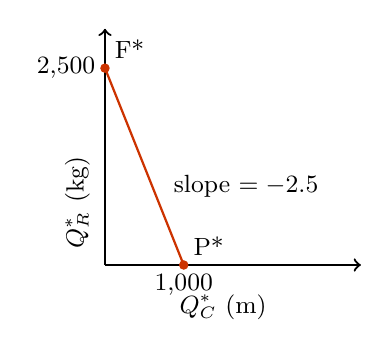
\begin{tikzpicture}[scale=0.5]
    % Axes
    \draw[->, thick] (0,0) -- (6.5,0);
    \draw[->, thick] (0,0) -- (0,6);
    
    % Axis labels
    \node[below] at (3,-0.5) {\small $Q^*_C$ (m)};
    \node[left, rotate=90] at (-0.7,3) {\small $Q^*_R$ (kg)};
    
    % PPF line (steeper)
    \draw[thick, foreigncolor] (0,5) -- (2,0);
    
    % Intercept labels
    \node[left] at (0,5) {\small 2,500};
    \node[below] at (2,0) {\small 1,000};
    
    % Slope annotation
    \node[right] at (1.5,2) {\small slope $= -2.5$};
    
    % F and P points (Thailand: F at y-intercept, P at x-intercept)
    \filldraw[foreigncolor] (0,5) circle (3pt);
    \filldraw[foreigncolor] (2,0) circle (3pt);
    \node[above right, font=\small] at (0,5) {F*};
    \node[above right, font=\small] at (2,0) {P*};
\end{tikzpicture}

\small{OC of cloth = 2.5 kg rice}
\end{column}
\end{columns}

\vspace{0.3cm}

\textbf{Slope of PPF} = $-\frac{\text{Max Rice}}{\text{Max Cloth}} = -\frac{a_{LC}}{a_{LR}}$ = \textbf{Opportunity cost of cloth}

\vspace{0.2cm}

\textbf{Comparing slopes:} India's PPF is \textit{flatter} $\Rightarrow$ lower OC of cloth $\Rightarrow$ \textbf{CA in cloth}

\end{frame}



%========================
% Transition to General Equilibrium
%========================

\begin{frame}{Transition: From PPF to Prices}

The PPF shows \textit{what} can be produced, but not \textit{what will be} produced.

\vspace{0.2cm}

\textbf{To determine production choices, we need prices.}

\vspace{0.2cm}

\textbf{Key assumptions:}
\begin{itemize}
    \item Individuals maximize income
    \item Labor moves to the sector with higher wages
    \item Perfect competition: Price = Cost = Wage $\times$ Unit labor requirement
    \item No profits, no market power
\end{itemize}

\vspace{0.2cm}

\textbf{In the absence of trade}, domestic relative prices equal relative unit labor requirements:

$$\frac{P_R}{P_C} = \frac{a_{LR}}{a_{LC}}$$

\vspace{0.2cm}

\small{If this weren't true, workers would move to the more profitable sector until prices adjust.}

\end{frame}


%========================
% Question 5: Relative Supply Curve - CORRECTED
% Thailand OC = 0.4 (lower, CA in rice) 
% India OC = 0.5 (higher, CA in cloth)
% On y-axis: 0.4 below 0.5
%========================

\begin{frame}{Question 5: Drawing the Relative Supply Curve}

Draw the Relative Supply (RS) curve with:
\begin{itemize}
    \item \textbf{Y-axis:} Relative price of rice vs cloth ($\frac{P_R}{P_C}$)
    \item \textbf{X-axis:} Relative quantity of rice vs cloth ($\frac{Q_R}{Q_C}$)
\end{itemize}

\vspace{0.5cm}

\textbf{Recall the opportunity costs of rice (in meters of cloth per kg):}
\begin{itemize}
    \item Thailand: $\frac{a_{LR}}{a_{LC}} = \frac{0.2}{0.5} = 0.4$ $\Rightarrow$ CA in rice
    \item India: $\frac{a_{LR}}{a_{LC}} = \frac{0.1}{0.2} = 0.5$ $\Rightarrow$ CA in cloth
\end{itemize}

\end{frame}

%------------------------
% Question 5: RS Step 1
%------------------------

\begin{frame}{Question 5: RS Curve --- Step 1}

\textbf{Draw the segment where $\frac{P_R}{P_C}$ equals Thailand's relative unit labor requirements. When is there no rice production at all?}

\vspace{0.1cm}

\centering
\begin{tikzpicture}[scale=0.75]
    % Axes
    \draw[->, thick] (0,0) -- (6,0) node[below] {$\frac{Q_R + Q^*_R}{Q_C + Q^*_C}$};
    \draw[->, thick] (0,0) -- (0,5) node[left] {$\frac{P_R}{P_C}$};
    
    % Thailand's OC line (flat segment at 0.4)
    \draw[thick, foreigncolor] (0,1.6) -- (3,1.6);
    
    % Label
    \node[left] at (0,1.6) {\small $\frac{a^*_{LR}}{a^*_{LC}} = 0.4$};
    
    % India's OC for reference (dashed)
    \draw[dashed, gray] (0,2.5) -- (1,2.5);
    \node[left, gray] at (0,2.5) {\small $0.5$};
\end{tikzpicture}

\begin{itemize}
    \item At $\frac{P_R}{P_C} = 0.4$: T is indifferent, produces any mix of both goods
    \item At $\frac{P_R}{P_C} = 0.4$: I fully specializes in cloth
    \item If $\frac{P_R}{P_C} < 0.4$: \textbf{No rice production at all} (price too low)
\end{itemize}

\end{frame}

%------------------------
% Question 5: RS Step 2
%------------------------

\begin{frame}{Question 5: RS Curve --- Step 2}

\textbf{Draw the segment where $\frac{P_R}{P_C}$ is above Thailand's (0.4) and below India's (0.5) unit labor requirements.}

\vspace{0.3cm}

\centering
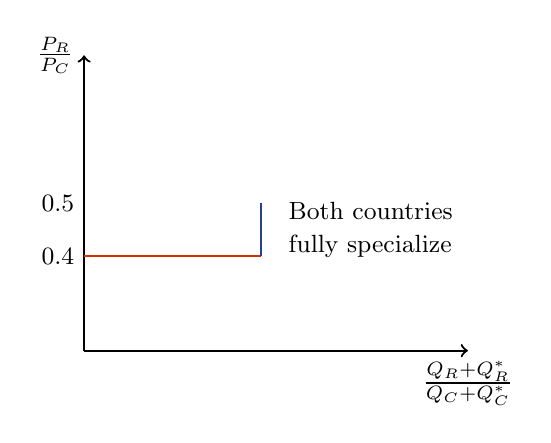
\begin{tikzpicture}[scale=0.75]
    % Axes
    \draw[->, thick] (0,0) -- (6.5,0) node[below] {$\frac{Q_R + Q^*_R}{Q_C + Q^*_C}$};
    \draw[->, thick] (0,0) -- (0,5) node[left] {$\frac{P_R}{P_C}$};
    
    % Thailand's OC line (flat segment at 0.4)
    \draw[thick, foreigncolor] (0,1.6) -- (3,1.6);
    
    % Vertical segment (both specialize)
    \draw[thick, myblue] (3,1.6) -- (3,2.5);
    
    % Labels
    \node[left] at (0,1.6) {\small $0.4$};
    \node[left] at (0,2.5) {\small $0.5$};
    
    % Annotation
    \node[right, align=left] at (3.3,2.05) {\small Both countries \\ \small fully specialize};
\end{tikzpicture}


\begin{itemize}
    \item T fully specializes in \textbf{rice} (its CA good)
    \item I fully specializes in \textbf{cloth} (its CA good)
    \item World relative supply of rice is \textbf{fixed} $\Rightarrow$ vertical segment
\end{itemize}

\end{frame}

%------------------------
% Question 5: RS Step 3
%------------------------

\begin{frame}{Question 5: RS Curve --- Step 3}

\textbf{Draw the segment where $\frac{P_R}{P_C}$ equals India's relative unit labor requirements (0.5).}

\vspace{0.1cm}

\centering
\begin{tikzpicture}[scale=0.75]
    % Axes
    \draw[->, thick] (0,0) -- (6.5,0) node[below] {$\frac{Q_R + Q^*_R}{Q_C + Q^*_C}$};
    \draw[->, thick] (0,0) -- (0,5) node[left] {$\frac{P_R}{P_C}$};
    
    % RS curve (three segments only)
    \draw[thick, foreigncolor] (0,1.6) -- (3,1.6);  % Thailand indifferent
    \draw[thick, myblue] (3,1.6) -- (3,2.5);        % Both specialize (vertical)
    \draw[thick, homecolor] (3,2.5) -- (7,2.5);     % India indifferent
    
    % Labels on y-axis
    \node[left] at (0,1.6) {\small $0.4$};
    \node[left] at (0,2.5) {\small $0.5$};


\end{tikzpicture}

\begin{itemize}
    \item I is indifferent, produces any mix of both goods
    \item T remains fully specialized in rice (its CA good)
    \item Relative supply can take any value $\Rightarrow$ \textbf{flat segment extending rightward}
\end{itemize}

\end{frame}


%========================
% Question 6: Relative Demand Curve
%========================

\begin{frame}{Question 6: Adding the Relative Demand Curve}

\textbf{Add the Relative Demand (RD) curve to the diagram.}

\vspace{0.3cm}

\begin{itemize}
    \item Draw \textbf{RD'} for the case where relative price equals Thailand's opportunity cost (0.4)
    \item Draw \textbf{RD} for the case where relative price is between 0.4 and 0.5
\end{itemize}

\end{frame}

%------------------------
% Question 6: Answer
%------------------------

\begin{frame}{Question 6: Answer --- RS and RD Equilibrium}

\centering
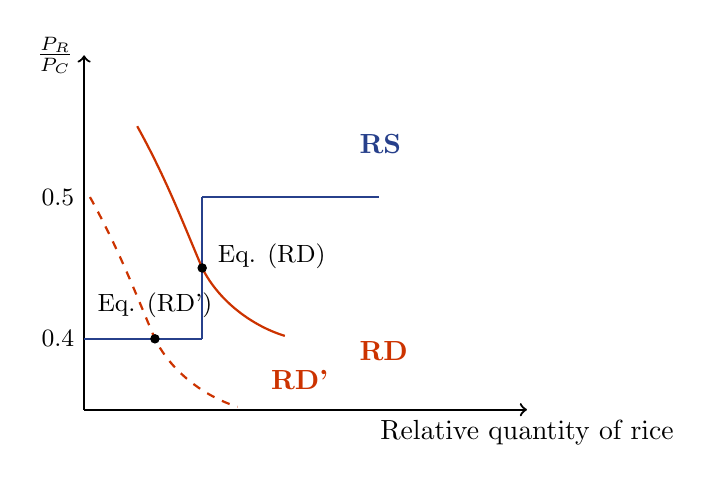
\begin{tikzpicture}[scale=0.75]
    % Axes
    \draw[->, thick] (0,0) -- (7.5,0) node[below] {Relative quantity of rice};
    \draw[->, thick] (0,0) -- (0,6) node[left] {$\frac{P_R}{P_C}$};
    
    % RS curve
    \draw[thick, myblue] (0,1.2) -- (2,1.2);
    \draw[thick, myblue] (2,1.2) -- (2,3.6);
    \draw[thick, myblue] (2,3.6) -- (5,3.6);
    
    % RD curve (slightly shorter on the right)
    \draw[thick, foreigncolor]
        (0.9,4.8) .. controls (1.4,3.9) and (1.7,3.1) .. (2,2.4)
        .. controls (2.3,1.8) and (2.9,1.4) .. (3.4,1.25);

    % RD' curve = shifted copy of RD (same curvature)
    \begin{scope}[shift={(-0.8,-1.2)}]
        \draw[thick, foreigncolor, dashed]
            (0.9,4.8) .. controls (1.4,3.9) and (1.7,3.1) .. (2,2.4)
            .. controls (2.3,1.8) and (2.9,1.4) .. (3.4,1.25);
    \end{scope}


    % Equilibrium point
    \filldraw[black] (2,2.4) circle (2pt);
    \node[right] at (2.1,2.6) {\small Eq. (RD)};
    
    % RD' equilibrium
    \filldraw[black] (1.2,1.2) circle (2pt);
    \node[above] at (1.2,1.4) {\small Eq. (RD')};
    
    % Labels
    \node[left] at (0,1.2) {\small $0.4$};
    \node[left] at (0,3.6) {\small $0.5$};
    
    % Curve labels
    \node[right, myblue] at (4.5,4.5) {\textbf{RS}};
    \node[right, foreigncolor] at (4.5,1) {\textbf{RD}};
    \node[right, foreigncolor] at (3,0.5) {\textbf{RD'}};
\end{tikzpicture}

\vspace{0.2cm}

\small{\textbf{RD'}: Equilibrium at Thailand's OC $\Rightarrow$ Thailand produces both goods.}

\small{\textbf{RD}: Equilibrium between OCs $\Rightarrow$ Both countries fully specialize.}

\end{frame}

%========================
% Question 8: Gains from Trade
%========================

\begin{frame}{Question 7: PPF and Gains from Trade}

\textbf{Draw a figure with the PPF before and after trade for each country.}

\vspace{0.3cm}

\begin{itemize}
    \item Start with the domestic PPF from Question 4
    \item Calculate the new consumption possibilities after trade
    \item In which goods do the gains from trade occur for each country?
\end{itemize}

\vspace{0.5cm}

\textbf{Assume:} World relative price settles at $\frac{P_R}{P_C} = 0.45$ (between 0.4 and 0.5)

\end{frame}


%========================
% Question 7: Gains from Trade - CORRECTED CALCULATIONS
%========================

\begin{frame}{Question 7: PPF and Gains from Trade}

\textbf{Draw a figure with the PPF before and after trade for each country.}

\vspace{0.3cm}

\begin{itemize}
    \item Start with the domestic PPF from Question 4
    \item Calculate the new consumption possibilities after trade
    \item In which goods do the gains from trade occur for each country?
\end{itemize}

\vspace{0.5cm}

\textbf{Assume:} World relative price settles at $\frac{P_R}{P_C} = 0.45$ 

\vspace{0.2cm}

\small{(This is between Thailand's OC of 0.4 and India's OC of 0.5, so both countries fully specialize.)}

\end{frame}

%------------------------
% Question 7: Understanding the world price
%------------------------

\begin{frame}{Question 7: Understanding the World Price}

\textbf{Given:} $\frac{P_R}{P_C} = 0.45$

\vspace{0.3cm}

\textbf{What does this mean?}

$$\frac{P_R}{P_C} = 0.45 \implies P_R = 0.45 \times P_C$$

\vspace{0.2cm}

\textbf{Or:} The price of 1 kg rice equals 0.45 times the price of 1 m cloth.

\vspace{0.2cm}

\textbf{This means:} Rice is relatively cheap, cloth is relatively expensive.

\vspace{0.5cm}

\textbf{Exchange rates on world markets:}

\begin{itemize}
    \item \textbf{1 m cloth} $\rightarrow$ $\frac{P_C}{P_R} = \frac{1}{0.45} = 2.22$ \textbf{kg rice}
    \item \textbf{1 kg rice} $\rightarrow$ $\frac{P_R}{P_C} = 0.45$ \textbf{m cloth}
\end{itemize}

\end{frame}

%------------------------
% Question 7: India's calculation
%------------------------

\begin{frame}{Question 7: Calculating India's Trade Line}

\textbf{India} specializes in \textbf{cloth} (produces at point F: 5,000 m cloth)

\vspace{0.3cm}

\textbf{If India trades ALL its cloth for rice:}

\vspace{0.2cm}

We know: 1 m cloth $\rightarrow$ 2.22 kg rice

\vspace{0.2cm}

\begin{align*}
\text{Max rice} &= \text{Cloth produced} \times \frac{P_C}{P_R} \\[0.3cm]
&= 5,000 \text{ m} \times 2.22 \frac{\text{kg}}{\text{m}} \\[0.3cm]
&= \textbf{11,111 kg rice}
\end{align*}

\vspace{0.3cm}

\textbf{India's trade line:}
\begin{itemize}
    \item X-intercept (point F): 5,000 m cloth (production point)
    \item Y-intercept (point T): 11,111 kg rice (max consumption if all cloth traded)
\end{itemize}

\end{frame}

%------------------------
% Question 7: Thailand's calculation
%------------------------

\begin{frame}{Question 7: Calculating Thailand's Trade Line}

\textbf{Thailand} specializes in \textbf{rice} (produces at point P*: 2,500 kg rice)

\vspace{0.3cm}

\textbf{If Thailand trades ALL its rice for cloth:}

\vspace{0.2cm}

We know: 1 kg rice $\rightarrow$ 0.45 m cloth

\vspace{0.2cm}

\begin{align*}
\text{Max cloth} &= \text{Rice produced} \times \frac{P_R}{P_C} \\[0.3cm]
&= 2,500 \text{ kg} \times 0.45 \frac{\text{m}}{\text{kg}} \\[0.3cm]
&= \textbf{1,125 m cloth}
\end{align*}

\vspace{0.3cm}

\textbf{Thailand's trade line:}
\begin{itemize}
    \item Y-intercept (point P*): 2,500 kg rice (production point)
    \item X-intercept (point T*): 1,125 m cloth (max consumption if all rice traded)
\end{itemize}

\end{frame}

%------------------------
% Question 7: India's Gains from Trade - Graph
%------------------------

\begin{frame}{Question 7: India's Gains from Trade}

\centering
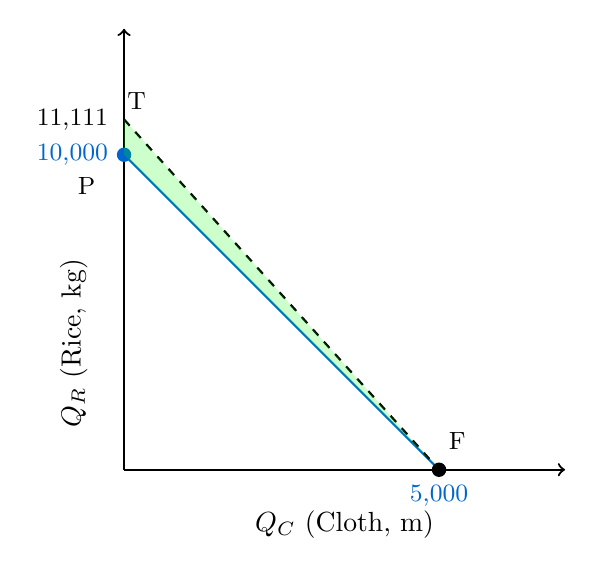
\begin{tikzpicture}[scale=0.8]
    % Axes
    \draw[->, thick] (0,0) -- (7,0);
    \draw[->, thick] (0,0) -- (0,7);
    
    % Axis labels
    \node[below] at (3.5,-0.5) {$Q_C$ (Cloth, m)};
    \node[left, rotate=90] at (-0.8,3.5) {$Q_R$ (Rice, kg)};
    
    % Original PPF (slope = -2): from (0,10000) to (5000,0), scaled: (0,5) to (5,0)
    \draw[thick, homecolor] (0,5) -- (5,0);
    \node[left, homecolor, font=\small] at (-0.1,5) {10,000};
    \node[below, homecolor, font=\small] at (5,-0.1) {5,000};
    
    % Trade line from F(5,0) to T(0, 11,111) - steeper than PPF
    % Scaled: 11,111 -> 5.56
    \draw[thick, dashed, black] (0,5.56) -- (5,0);
    \node[left, font=\small] at (-0.1,5.56) {11,111};
    
    % Points
    \filldraw[homecolor] (0,5) circle (3pt);
    \node[left, font=\small] at (-0.3,4.5) {P};
    
    \filldraw[black] (5,0) circle (3pt);
    \node[below right, font=\small] at (5,0.75) {F};
    
    \node[above left, font=\small] at (0.5,5.56) {T};
    
    % Shaded gain area
    \fill[green, opacity=0.2] (0,5) -- (0,5.56) -- (5,0) -- cycle;
    
\end{tikzpicture}
\vspace{-0.25cm}
\begin{itemize}
    \item Autarky max rice (point P): 10,000 kg
    \item Trade max rice (point T): 11,111 kg
    \item \textbf{Gain: +1,111 kg rice} (+11\% in rice consumption)
\end{itemize}

\end{frame}

%------------------------
% Question 7: Thailand's Gains from Trade - Graph
%------------------------

\begin{frame}{Question 7: Thailand's Gains from Trade}

\centering
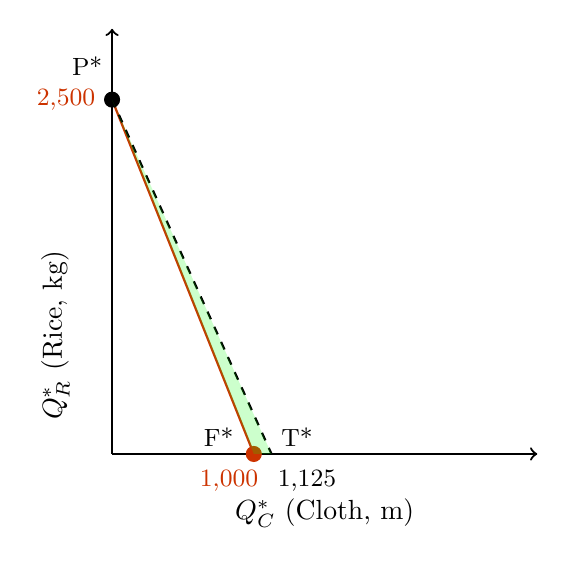
\begin{tikzpicture}[scale=0.9]
    % Axes
    \draw[->, thick] (0,0) -- (6,0);
    \draw[->, thick] (0,0) -- (0,6);
    
    % Axis labels
    \node[below] at (3,-0.5) {$Q^*_C$ (Cloth, m)};
    \node[left, rotate=90] at (-0.8,3) {$Q^*_R$ (Rice, kg)};
    
    % Original PPF (slope = -2.5): from (0,2500) to (1000,0)
    % Scaled: 2500->5, 1000->2, 1125->2.25
    \draw[thick, foreigncolor] (0,5) -- (2,0);
    \node[left, foreigncolor, font=\small] at (-0.1,5) {2,500};
    \node[below, foreigncolor, font=\small] at (1.65,-0.1) {1,000};
    
    % Trade line from P*(0,2500) to T*(1125,0) - flatter than PPF
    % Scaled: 1125 -> 2.25
    \draw[thick, dashed, black] (0,5) -- (2.25,0);
    \node[below, font=\small] at (2.75,-0.1) {1,125};
    
    % Points
    \filldraw[black] (0,5) circle (3pt);
    \node[above left, font=\small] at (0,5.2) {P*};
    
    \filldraw[foreigncolor] (2,0) circle (3pt);
    \node[below left, font=\small] at (1.85,0.5) {F*};
    
    \node[below right, font=\small] at (2.25,0.5) {T*};
    
    % Shaded gain area
    \fill[green, opacity=0.2] (0,5) -- (2,0) -- (2.25,0) -- cycle;
    
\end{tikzpicture}

\vspace{-0.2cm}

\begin{itemize}
    \item Autarky max cloth (point F*): 1,000 m
    \item Trade max cloth (point T*): 1,125 m
    \item \textbf{Gain: +125 m cloth} (+12.5\% in cloth consumption)
\end{itemize}

\end{frame}

%========================
% Slide: Model Limitations
%========================

\begin{frame}{Limitations of the Ricardian Model}

\textbf{What the model gets right:}
\begin{itemize}
    \item Countries export goods where they have \textit{relatively} high productivity
    \item Trade benefits all countries (mutual gains)
\end{itemize}

\vspace{0.5cm}

\textbf{What the model misses:}
\begin{enumerate}
    \item \textbf{Extreme specialization} --- Reality shows incomplete specialization
    \item \textbf{Income distribution} --- Model assumes everyone gains; in reality, trade creates winners and losers
    \item \textbf{Factor endowments} --- Only labor matters; ignores capital, land
    \item \textbf{Economies of scale} --- Cannot explain trade between similar countries
    \item \textbf{Transport costs} --- Model assumes zero trade costs
\end{enumerate}
\end{frame}

%========================
% Reflection Questions: Conceptual Implications & Limitations
%========================

\begin{frame}{Questions for Reflection: Conceptual Implications \& Limitations of the Ricardian Model}

\small

\begin{enumerate}
    \item How do the incentives to trade change for small vs large countries? Please respond a) with reference to economies of scale, b) endowment differences.
    
    \vspace{0.2cm}
    
    \item What are the limits of the Ricardian view that all international trade is due to differences in labor productivity? Please respond with references to natural resources, transport costs, cultural proximity.
    
    \vspace{0.2cm}
    
    \item One crucial assumption of the Ricardian model is that labor can freely move between activities. Using the Korean movie \textit{No Other Choice} (or another example of your choice), explain why this assumption may not hold in reality and reflect upon the trade-off between gains from trade and labor adjustment costs. What must hold true for net welfare improvements? What role do non-pecuniary factors like culture, history, identity play, and should they be considered in the economic definition of welfare or not?
\end{enumerate}

\end{frame}

\begin{frame}{Questions for Reflection (continued)}

\small

\begin{enumerate}
    \setcounter{enumi}{3}
    
    \item Another crucial assumption of the Ricardian model is full employment and no monopsony power. Workers earn the market price of output of their labor. How would monopsony power affect the distribution of gains from trade among labor and capital?
    
    \vspace{0.3cm}
    
    \item Transport costs have become negligible in contemporary trade for most consumer goods. Explain, using an example, whether this strengthens the Ricardian logic of trade integration.
    
    \vspace{0.3cm}
    
    \item Use the same reasoning as for transport costs, but explain how a country could strategically use a tariff instead of transport cost.
    
\end{enumerate}

\end{frame}


%========================
% Slide: Summary
%========================

\begin{frame}{Summary: Key Takeaways}

\begin{enumerate}
    \item \textbf{Comparative advantage}, not absolute advantage, determines trade patterns
    
    \vspace{0.3cm}
    
    \item Comparative advantage is determined by \textbf{opportunity costs} (relative unit labor requirements)
    
    \vspace{0.3cm}
    
    \item Trade allows countries to consume \textbf{beyond their PPF}
    
    \vspace{0.3cm}
    
    \item \textbf{Relative wages} are determined by relative productivity and lie between countries' productivity ratios
    
    \vspace{0.3cm}
    
    \item \textbf{All countries gain} from trade, regardless of their absolute productivity levels
\end{enumerate}

\vspace{0.5cm}

\textit{Next week: Heckscher-Ohlin Factor Endowment model.}

\end{frame}


% \subsection{Heckscher-Ohlin}


% \section{Environmental Economics}

% \subsection{Namur Audition}

% \begin{frame}

% \vspace{1.0cm}

% \centering
% {\Large \textbf{Florian Münch}} \\[0.3cm]

% {\small London School of Economics \\ (Chercheur postdoctoral, projet \textit{Productive and Inclusive Net Zero})} \\ 
% \& \\
% {\small King’s College London \\ (Responsable de module en économie environnementale)} \\[0.6cm]

% {\small Audition pour le poste de Professeur assistant en économie} \\
% {\small Université de Namur, 26 janvier 2026}

% \vfill

% \end{frame}

% \begin{frame}{Structure de la Présentation}
% \begin{enumerate}
%     \item Présentation pédagogique : \textit{Régulation de la pollution sous incertitude (Weitzman, 1974)}  \\~\\
%     \item Présentation de recherche : \textit{Stronger Together? Female Export Consortia}  \\~\\
%     \item Programme de recherche
% \end{enumerate}
% \end{frame}


% \begin{frame}{Présentation pédagogique: Agenda}

% \textbf{Sujet :} La régulation de la pollution sous incertitude \\ (Martin Weitzman 1974 \textit{Prix vs Quantités})

% \begin{enumerate}
%     \item La pollution comme une externalité qui entraine une défaillance du marché et un excès de production \\~\\
%     \item La problèmatique de Weitzman : réguler la pollution par les prix ou par les quantités ? \\~\\
%     \item Résultat clé : le choix de l’instrument dépend de la relation entre coûts de réduction \& dommages liées a la pollution
% \end{enumerate}

% \end{frame}


% \begin{frame}{Pourquoi s'intéresser a la pollution?}
% \begin{itemize}
%     \item Depuis la révolution industrielle: Croissance économique et hausse des revenus et du bien-être matériel sans précédent \\~\\
    
%     \item Accompagnée également d’une pollution environnementale inédite \\~\\

%     \item Conséquences massives pour les humains (santé) \& la nature (climat, biodiversité) \\~\\
    
%     \item Vue économique de la pollution : \textbf{externalité}
%         \begin{itemize}
%             \item Définition: Les actions d'un agent affecte le bien-être des tiers sans en prendre compte dans ses décisions
%             \item En conséquence, les decisions des acteurs du marché entraine un excès de pollution
%         \end{itemize}
% \end{itemize}
% \end{frame}



% %========================
% % Slide: Externality
% %========================

% \begin{frame}{L'externalité et la surproduction (et la surpollution)}
% \centering
% \begin{tikzpicture}[scale=1.1]

% % Paramètres
% \pgfmathsetmacro{\mD}{-0.7}    % pente demande (négative)
% \pgfmathsetmacro{\bD}{4.5}     % intercept demande
% \pgfmathsetmacro{\mS}{0.6}     % pente offre (CMP)
% \pgfmathsetmacro{\bS}{0.3}     % intercept offre
% \pgfmathsetmacro{\dm}{1.4}     % décalage vertical pour CMS

% % Points d'équilibre
% % Marché : Demande = Offre (CMP)
% \pgfmathsetmacro{\Qm}{(\bD-\bS)/(\mS-\mD)}
% \pgfmathsetmacro{\Pm}{\mS*\Qm+\bS}

% % Optimal : Demande = CMS
% \pgfmathsetmacro{\Qstar}{(\bD-\bS-\dm)/(\mS-\mD)}
% \pgfmathsetmacro{\Pstar}{\mS*\Qstar+\bS+\dm}

% % Point sur CMS à Qm (pour le triangle)
% \pgfmathsetmacro{\CMSatQm}{\mS*\Qm+\bS+\dm}

% % Axes
% \draw[->, thick] (0,0) -- (6,0) node[below] {Quantité};
% \draw[->, thick] (0,0) -- (0,5.5) node[left] {Prix};

% % Courbe de demande B'(Q)
% \draw[thick, black] (0.3, {\mD*0.3+\bD}) -- (5.5, {\mD*5.5+\bD});
% \node[black, align=left] at (1.5, {\mD*0.5+\bD+0.7}) {\textbf{Demande} $B'(Q)$ \\ \small Utilité marginale};

% % Courbe d'offre CMP = C'(Q)
% \draw[thick, blue] (0.3, {\mS*0.3+\bS}) -- (5.5, {\mS*5.5+\bS});
% \node[blue, align=left] at (7, {\mS*5.0+\bS}) {\textbf{Offre} $C'(Q)$ \\ \small Coûts marginaux \\ \small privés = CMP};

% % Qm et Pm - équilibre de marché (slide 1 uniquement)
% \onslide<1>{
% \draw[dashed, gray] (\Qm, 0) -- (\Qm, \Pm);
% \node[below] at (\Qm, 0) {$Q^m$};
% \draw[dashed, gray] (0, \Pm) -- (\Qm, \Pm);
% \node[left] at (0, \Pm) {$P^m$};
% \filldraw[black] (\Qm, \Pm) circle (2pt);

% % Label B'(Q) = C'(Q) au-dessus du point d'intersection (slide 1 uniquement)
% \node[above] at (\Qm, \Pm + 0.7) {$B'(Q) = C'(Q)$};
% }

% % === Slide 2: Ajout CMS et tout le reste ===
% \onslide<2->{

% % Courbe CMS = CMP + DM (coûts marginaux sociaux)
% \draw[thick, green!60!black] (0.3, {\mS*0.3+\bS+\dm}) -- (5.5, {\mS*5.5+\bS+\dm});
% \node[green!60!black, align=left] at (6.8, {\mS*5.0+\bS+\dm+0.5}) {Coûts marginaux \\ sociaux \\ \small $CMS = CMP + DM$};

% % Triangle de perte de bien-être (DWL)
% \fill[red!70, opacity=0.6]
%   (\Qstar, \Pstar) -- (\Qm, \Pm) -- (\Qm, \CMSatQm) -- cycle;


% % Flèche et label DWL
% \draw[->, thick, red!70!black] ({\Qm + 0.3}, {\CMSatQm + 1.15}) -- ({\Qm - 0.15}, {\CMSatQm + 0.1});
% \node[red!70!black, align=center] at ({\Qm + 0.5}, {\CMSatQm + 1.5}) {Perte de \\ bien-être};

% % Q* et P*
% \draw[dashed, gray] (\Qstar, 0) -- (\Qstar, \Pstar);
% \node[below] at (\Qstar, 0) {$Q^*$};
% \draw[dashed, gray] (0, \Pstar) -- (\Qstar, \Pstar);
% \node[left] at (0, \Pstar) {$P^*$};

% % Qm - ligne verticale jusqu'à CMS
% \draw[dashed, gray] (\Qm, 0) -- (\Qm, \CMSatQm);
% \node[below] at (\Qm, 0) {$Q^m$};
% \draw[dashed, gray] (0, \Pm) -- (\Qm, \Pm);
% \node[left] at (0, \Pm) {$P^m$};

% % Flèche double entre CMP et CMS pour montrer DM
% \pgfmathsetmacro{\xDM}{4.5}
% \pgfmathsetmacro{\yCMP}{\mS*\xDM+\bS}
% \pgfmathsetmacro{\yCMS}{\mS*\xDM+\bS+\dm}
% \draw[<->, thick, purple] (\xDM, \yCMP) -- (\xDM, \yCMS);
% \node[purple, right] at (\xDM + 0.1, {(\yCMP+\yCMS)/2}) {$DM$};

% % Points d'intersection
% \filldraw[black] (\Qstar, \Pstar) circle (2pt);
% \filldraw[black] (\Qm, \Pm) circle (2pt);
% \filldraw[black] (\Qm, \CMSatQm) circle (2pt);

% }

% \end{tikzpicture}
% \end{frame}

% % A dire
% % Niveau de production du marche plus elevee que le niveau de production optimal
% % Ceci est liee au fait que les producteurs ne prennent en compte que leur couts marginaux de production, et n'est pas les couts externent, p.ex. tous les couts medicaux causes par la prooduction, dans leur choice du q optimal. 

% % Nous, autant qu'economistes, considerent ceci une defaillance de marche, car les droits de propriete ne sont pas complets; autrements dit, les producteurs n'internalisent qu'une partie des couts qu'ils causent

% % La defaillance de marche justifie l'intervention de l'etat pour reduire le niveau de production (et de pollution liee a la production) au niveau optimal


% %========================
% % Slide: Weitzman 1 + MAC-MD definition
% %========================

% % \begin{frame}{Externalité environnementale et défaillance du marche: Comment atteindre le niveau optimal de pollution ?}

% % \begin{itemize}
% %     \item<1-> \textbf{Définition économique du niveau optimal de la pollution:}
% %     \begin{itemize}
% %         \item<1-> $C'(Q) = B'(Q) $
% %         \item<1-> \textit{Attention}: Q = pollution
% %         \item<1-> $C'(Q)$: coûts marginaux d’abattement (CMA) 
% %         \item<1-> $B'(Q) $: dommage marginal (bénéfices marginaux d’abattement (BMA))
% %     \end{itemize}
% % \end{itemize}

% % \end{frame}

% % A dire:
% % ds l'equilibre, les couts de reduction de la pollution sont egale au dommage cause

% % \begin{frame}{Le problème: Comment atteindre l'optimum social de pollution?}

% % \only<1>{
% % \begin{itemize}
% %     \item<1-> \textbf{Weitzman (1974) : deux options pour controler la pollution}
% %     \begin{enumerate}
% %         \item<1-> Réguler le prix
% %         \item<1-> Réguler la quantité
% %     \end{enumerate}        
% % \end{itemize}
% % }
% % \end{frame}

% \begin{frame}{Comment atteindre l'optimum social de pollution? \\ }
% \centering
% \begin{tikzpicture}[scale=1.2]

% % Paramètres
% \pgfmathsetmacro{\m}{0.5}   % pente
% \pgfmathsetmacro{\bA}{0.8}  % intercept CMA
% \pgfmathsetmacro{\k}{3.8}   % intercept DM

% % Intersection CMA = DM (optimum social)
% \pgfmathsetmacro{\Rstar}{(\k-\bA)/(2*\m)}
% \pgfmathsetmacro{\Pstar}{\m*\Rstar+\bA}

% % Niveau de marché (Rm < R*)
% \pgfmathsetmacro{\Rm}{\Rstar-1.2}
% \pgfmathsetmacro{\Pm}{\m*\Rm+\bA}

% % Axes (toujours visibles)
% \draw[->, thick] (0,0) -- (5.5,0) node[below] {Réduction de la pollution};
% \draw[->, thick] (0,0) -- (0,5.5) node[above] {Coût / Dommage};



% % -----------------------------------
% % 1) CMA seule
% % -----------------------------------
% \onslide<2->{
% \draw[thick, blue] (0.5, {\m*0.5+\bA}) -- (5.5, {\m*5.5+\bA});
% \node[blue] at (5.6, {\m*5.5+\bA+0.25}) {Coûts marginaux de réduction (CMA)};
% }
% % -----------------------------------
% % 2) DM seul
% % -----------------------------------
% \onslide<3->{
% \draw[thick, red] (0.5, {\k-\m*0.5}) -- (5.5, {\k-\m*5.5});
% \node[red] at (5.6, {\k-\m*5.5-0.25}) {Dommages marginaux (DM)};
% }

% % -----------------------------------
% % 3) Optimum social (R*, P*, CMA = DM)
% % -----------------------------------
% \onslide<4->{
% % Point optimal
% \filldraw[black] (\Rstar,\Pstar) circle (2pt);
% % R*
% \draw[dashed] (\Rstar,0) -- (\Rstar,\Pstar);
% \node[below] at (\Rstar,0) {$R^*$};
% % P*
% \draw[dashed] (0,\Pstar) -- (\Rstar,\Pstar);
% \node[left] at (0,\Pstar) {$P^*$};
% }

% % Label CMA = DM au-dessus du point d'intersection (version 4 uniquement)
% \onslide<4>{
% \node[above] at (\Rstar, \Pstar + 0.4) {$CMA = DM$};
% }

% % -----------------------------------
% % 4) Niveau de marché (Rm, Pm)
% % -----------------------------------
% \onslide<5->{
% % Point de marché
% \filldraw[black] (\Rm,\Pm) circle (2pt);
% % Rm
% \draw[dashed] (\Rm,0) -- (\Rm,\Pm);
% \node[below] at (\Rm,0) {$R_m$};
% % Pm
% \draw[dashed] (0,\Pm) -- (\Rm,\Pm);
% \node[left] at (0,\Pm) {$P_m$};
% }

% \end{tikzpicture}

% \end{frame}



% \begin{frame}{Prix ou quantité ? La problématique de Weitzman (1974)}
% \centering
% \begin{tikzpicture}[scale=1.2]
% % Paramètres
% \pgfmathsetmacro{\m}{0.5}
% \pgfmathsetmacro{\bA}{0.8}
% \pgfmathsetmacro{\k}{3.8}
% % Intersection CMA = DM (optimum social)
% \pgfmathsetmacro{\Rstar}{(\k-\bA)/(2*\m)}
% \pgfmathsetmacro{\Pstar}{\m*\Rstar+\bA}
% % Niveau de marché (Rm < R*)
% \pgfmathsetmacro{\Rm}{\Rstar-1.2}
% \pgfmathsetmacro{\Pm}{\m*\Rm+\bA}
% % Axes
% \draw[->, thick] (0,0) -- (6.4,0) node[below] {Réduction de la pollution};
% \draw[->, thick] (0,0) -- (0,5.8) node[above] {Coût / Dommage};
% % CMA
% \draw[thick, blue] (0.5, {\m*0.5+\bA}) -- (5.5, {\m*5.5+\bA});
% \node[blue] at (5.6, {\m*5.5+\bA+0.25}) {CMA};
% % DM
% \draw[thick, red] (0.5, {\k-\m*0.5}) -- (5.5, {\k-\m*5.5});
% \node[red] at (5.6, {\k-\m*5.5-0.25}) {DM};
% % Point optimal
% \filldraw[black] (\Rstar,\Pstar) circle (2pt);
% % Lignes pointillées standard (gris)
% \draw[dashed, gray] (\Rstar,0) -- (\Rstar,\Pstar);
% \draw[dashed, gray] (0,\Pstar) -- (\Rstar,\Pstar);
% % Point de marché
% \filldraw[black] (\Rm,\Pm) circle (2pt);
% \draw[dashed, gray] (\Rm,0) -- (\Rm,\Pm);
% \draw[dashed, gray] (0,\Pm) -- (\Rm,\Pm);
% \node[below] at (\Rm,0) {$R_m$};
% \node[left] at (0,\Pm) {$P_m$};

% % -----------------------------------
% % 1) Quantité (ligne verticale en vert)
% % -----------------------------------
% \onslide<1>{
% \draw[dashed, very thick, green!70!black] (\Rstar,0) -- (\Rstar,\Pstar);
% \node[below, green!70!black] at (\Rstar,0) {$R = R^*$};
% \node[left] at (0,\Pstar) {$P^*$};
% }

% % -----------------------------------
% % 2) Prix (ligne horizontale en vert)
% % -----------------------------------
% \onslide<2>{
% \draw[dashed, very thick, green!70!black] (0,\Pstar) -- (\Rstar,\Pstar);
% \node[below] at (\Rstar,0) {$R^*$};
% \node[left, green!70!black] at (0,\Pstar) {$P = P^*$};
% }

% % -----------------------------------
% % 3) Prix + Quantité + ?
% % -----------------------------------
% \onslide<3>{
% \draw[dashed, very thick, green!70!black] (\Rstar,0) -- (\Rstar,\Pstar);
% \draw[dashed, very thick, green!70!black] (0,\Pstar) -- (\Rstar,\Pstar);
% \node[below, green!70!black] at (\Rstar,0) {$R = R^*$};
% \node[left, green!70!black] at (0,\Pstar) {$P = P^*$};
% \node[green!70!black, font=\Huge\bfseries] 
% at (\Rstar,\Pstar) [yshift=1cm] {?};
% }

% \end{tikzpicture}
% \end{frame}


% % \begin{frame}{Externalité environnementale et défaillance du marche: Comment atteindre l’optimum de pollution ?}

% % \begin{itemize}
% %     \item<1-> \textbf{Définition économique du niveau optimal de pollution :}
% %     \begin{itemize}
% %         \item<1-> $C'(Q) = B'(Q) $
% %         \item<1-> \textit{Attention}: Q = pollution
% %         \item<1-> $C'(Q)$: coûts marginaux d’abattement (CMA) 
% %         \item<1-> $B'(Q) $: dommage marginal (bénéfices marginaux d’abattement (BMA))
% %     \end{itemize}

% %     \vspace{0.4cm}
    
% %     \item<1-> \textbf{Weitzman (1974) : deux options}
% %     \begin{enumerate}
% %         \item<1-> Réguler le prix
% %         \item<1-> Réguler la quantité
% %     \end{enumerate}
% % \end{itemize}

% % \end{frame}


% %========================
% % Slide: MAC-MD plus quantity and price regulation
% %========================
% % \begin{frame}{Reduction (Abattement) des Pollutions: Par Quantite ou Prix?}

% % \centering
% % \only<1>{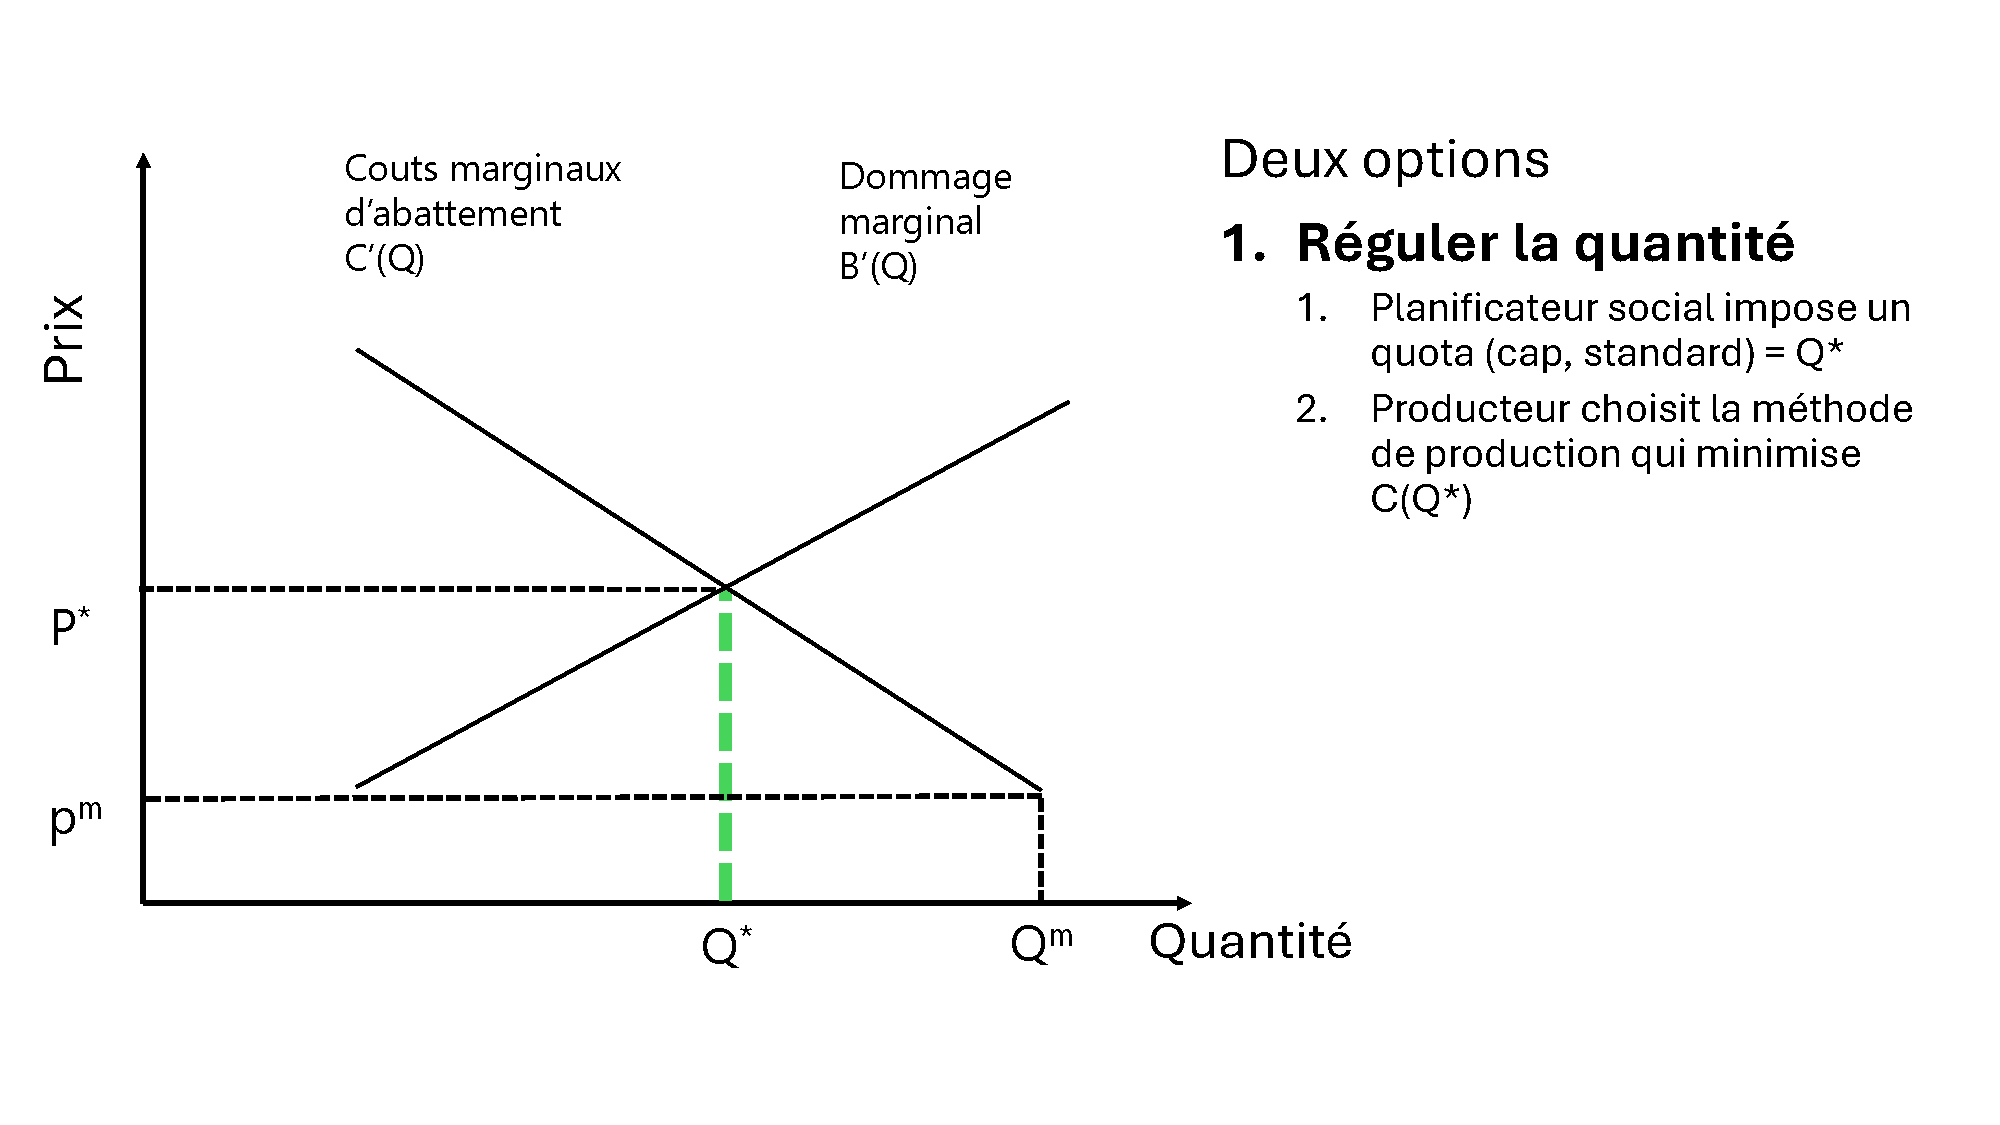
\includegraphics[width=1.05\textwidth]{mac_md_curves/mac_md_quantite.pdf}}
% % \only<2>{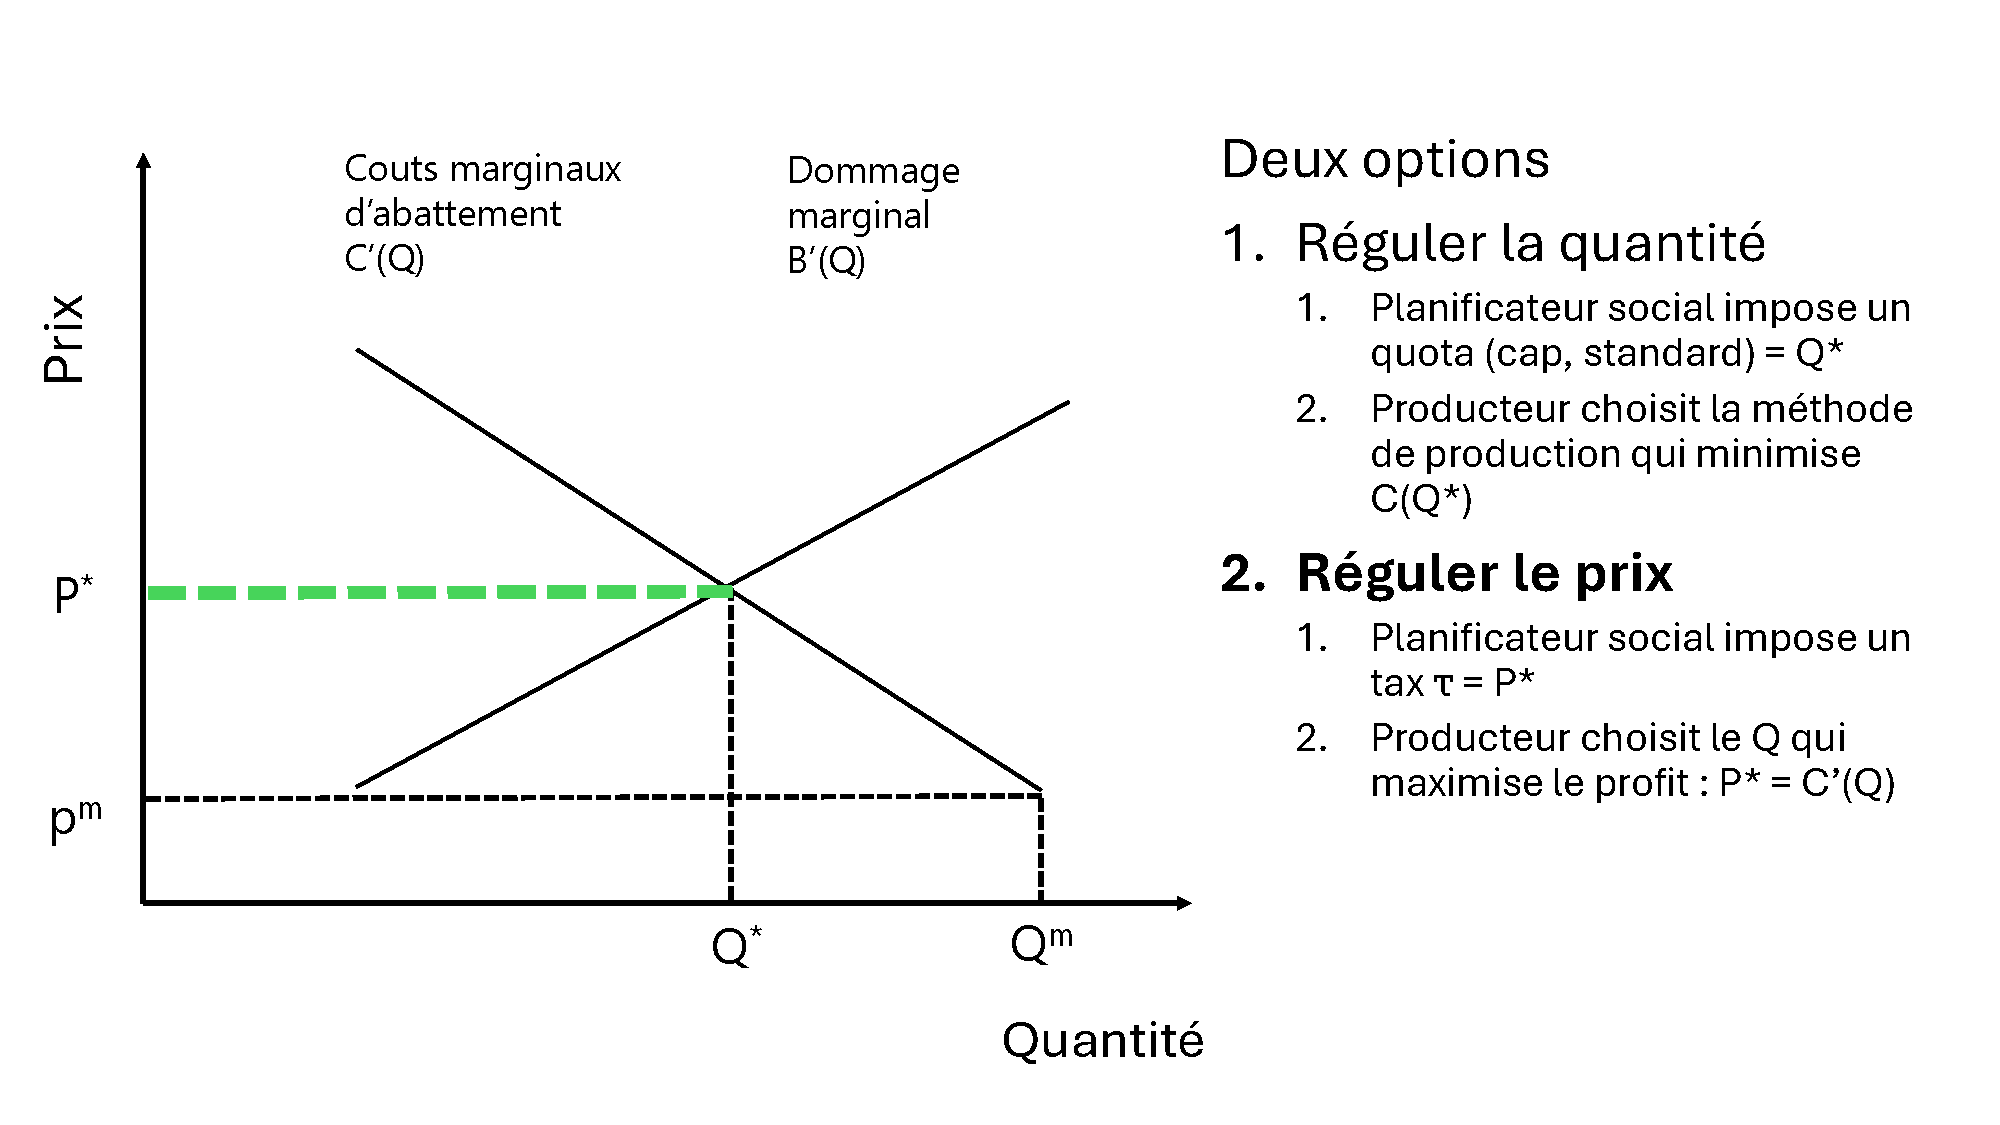
\includegraphics[width=1.05\textwidth]{mac_md_curves/mac_md_prix.pdf}}
% % \only<3>{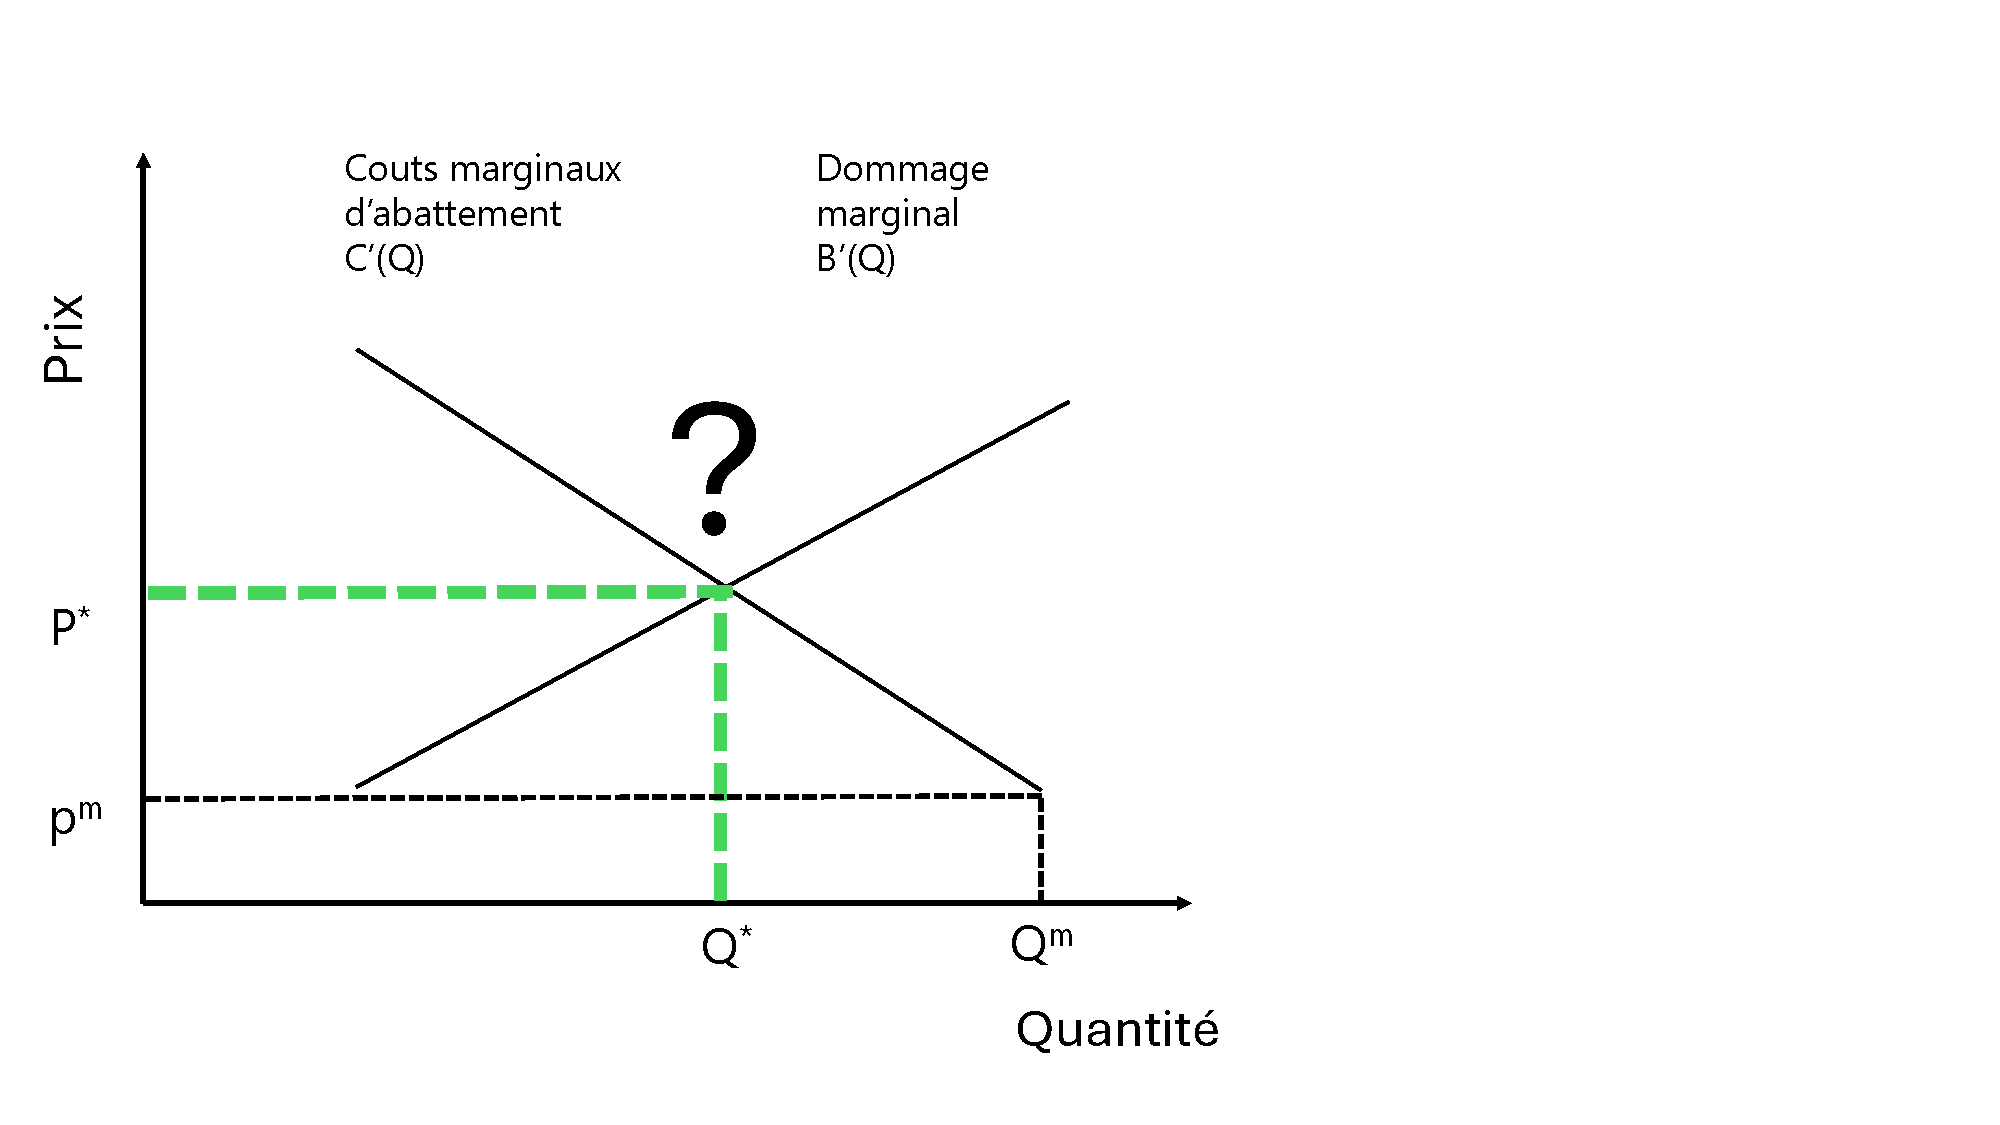
\includegraphics[width=1.05\textwidth]{mac_md_curves/mac_md_question.pdf}
% %     \item \textbf{Question de savoir :} la régulation par les prix ou par les quantités est-elle plus efficace pour contrôler la pollution ?
% % }
% % \end{frame}


% % \begin{frame}{Externalité environnementale et défaillance du marche: Comment atteindre l’optimum social ?}

% % \begin{itemize}
% %     \item \textbf{Définition économique de l’optimum social :}
% %     \begin{itemize}
% %         \item $B'(Q) = C'(Q)$
% %         \item Équilibrer les coûts marginaux d’abattement (CMA) et les bénéfices marginaux d’abattement (BMA)
% %     \end{itemize}

% %     \vspace{0.4cm}
    
% %     \item \textbf{Weitzman (1974) : deux options}
% %     \begin{enumerate}
% %         \item Réguler le prix
% %         \item Réguler la quantité
% %     \end{enumerate}

% %     \vspace{0.4cm}

% %     \item \textbf{Question de savoir :} la régulation par les prix ou par les quantités est-elle plus efficace pour contrôler la pollution ?
% % \end{itemize}

% % \end{frame}


% % \begin{frame}{Weitzman (1974) : rôle de $B''$ et $C''$}

% % \centering
% % \begin{tikzpicture}[scale=1.1]

% % % Axes
% % \draw[->] (0,0) -- (6,0) node[right] {Abattement $q$};
% % \draw[->] (0,0) -- (0,4.5) node[above] {Coût / Bénéfice marginal};

% % % MAC curve (upward sloping, convex)
% % \draw[thick, blue, domain=0.2:5.5, smooth] plot (\x, {0.3 + 0.1*\x + 0.08*\x*\x});
% % \node[blue] at (5.2,4.1) {MAC $= C'(q)$};
% % \node[blue] at (4.2,3.2) {$C''>0$};

% % % MB curve (downward sloping, concave)
% % \draw[thick, red, domain=0.2:5.5, smooth] plot (\x, {4.2 - 0.5*\x - 0.05*\x*\x});
% % \node[red] at (5.1,0.7) {MB $= B'(q)$};
% % \node[red] at (3.2,2.0) {$B''<0$};

% % % Intersection point
% % \draw[dashed] (2.6,0) -- (2.6,2.2);
% % \draw[dashed] (0,2.2) -- (2.6,2.2);
% % \filldraw (2.6,2.2) circle (2pt);

% % \node at (2.6,-0.3) {$q^*$};
% % \node at (-0.4,2.2) {$MAC=MB$};

% % \end{tikzpicture}

% % \vspace{0.3cm}

% % \textbf{Weitzman :} sous incertitude, le choix entre prix et quantités dépend de la courbure relative des fonctions de coûts et de bénéfices, c’est-à-dire de $C''$ et $B''$.

% % \end{frame}




% %========================
% % Slide B: Uncertainty
% %========================

% \begin{frame}{Incertitude sur les coûts de reduction \& les dommages de la pollution}

% \begin{itemize}
%   \item<1-> En cas d'information parfaite, $q^*$ et $p^*$ sont connus et la régulation par prix ou quantité est équivalente.
  
%   \item<2-> En réalité, le planificateur social manque d'information \& les C\&B d'abattement de la pollution sont incertains :
%   \[
%   CMA(q,\textcolor{blue}{\theta}) \quad ; \quad DM(q,\textcolor{red}{\eta}),
%   \]
%   où \textcolor{blue}{$\theta$} et \textcolor{red}{$\eta$} représentent des paramètres d'incertitude.
% \end{itemize}

% \vspace{0.2cm}

% \onslide<3->{
% \textbf{Implication :}
% \begin{itemize}
%   \item<3-> Le planificateur social prend donc des décisions approximatifs, nécessairement imparfaites (sous-optimales).
%   \item<4-> Ex.: $p_r<p*$: excès de pollution; $q_r < q*$: excès des coûts.
%   \item<5-> Arbitrage: fixer $p_r$: "certitude des coûts" et fixer $q_r$ "certitude des dommages".

% \end{itemize}
% }

% \end{frame}



% %========================
% % Slide D+E: Comparison and approximation
% %========================
% \begin{frame}{Comparer les instruments prix et quantité}
% %----------------------------------
% % Step 1: simple criterion + Wprix
% %----------------------------------
% \onslide<1->{
% \textbf{Critère de comparaison $\Delta$ ("perte relative de bien-être")}
% \vspace{0.05cm}
% \[
% \Delta = W^{\text{prix}} - W^{\text{quantité}}
% \]
% }
% \onslide<2->{
% \vspace{-0.2cm} % réduit l'espace entre les deux formules
% \[
% \text{où } W^{prix} = \mathbb{E}\Big[B\big(q(p,\textcolor{red}{\eta})\big) - C\big(q(p,\textcolor{blue}{\theta}),\textcolor{blue}{\theta}\big)\Big].
% \]
% }
% %----------------------------------
% % Step 2: definition of W^{prix}
% %----------------------------------
% \only<3>{  % Changed from \onslide to \only
% \vspace{-0.6cm} % réduit l'espace avant itemize
% \begin{itemize}
%   \item $\Delta > 0$ : la régulation par les prix est préférable.
%   \item $\mathbb{E}$ : L'espérance du bien-être moyen sur l'ensemble des réalisations r possibles des C\&B.
% \end{itemize}
% \vspace{0.2cm}
% }
% %----------------------------------
% % Step 3: Taylor approximation
% %----------------------------------
% \onslide<4->{
% \textbf{Approximation locale de $\Delta$ ("perte relative de bien-être")}
% \vspace{0.05cm}
% \[
% \Delta \approx \frac{\sigma^2}{2(C'')^2}\big(B'' + C''\big).
% \]
% \begin{itemize}
%   \item $C''$ : pente des coûts marginaux d'abattement (CMA),
%   \item $B''$ : pente des dommages marginaux (DM).
% \end{itemize}
% \vspace{0.05cm}
% \textbf{Résultat:}  
% $B'' + C''$ détermine l'instrument optimal.
% }
% \end{frame}

% %========================
% % Slide: Visualization of steep vs flat MAC & MD curves
% %========================
% % \begin{frame}{B'' et C'' visualisée: }


% % \centering
% % \only<1>{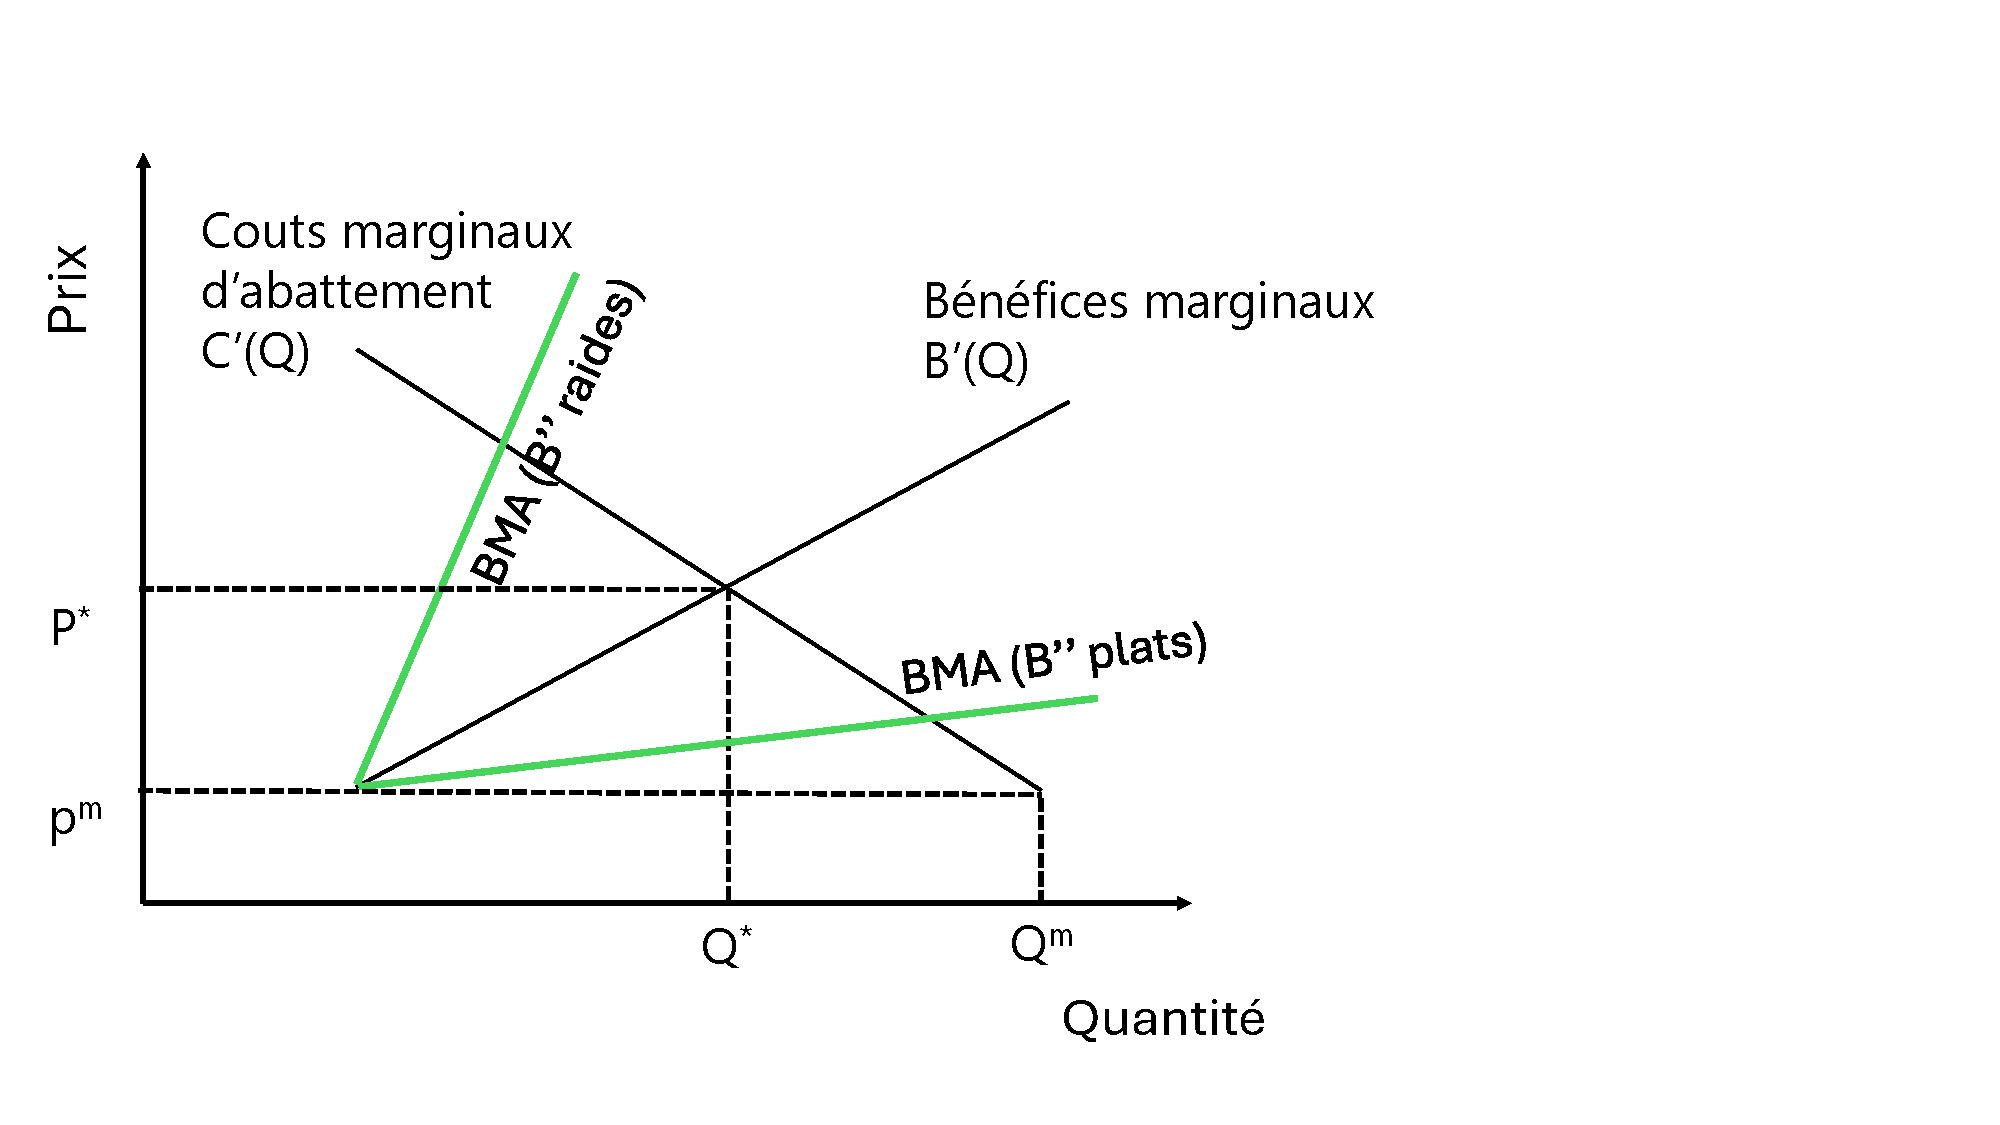
\includegraphics[width=1.1\textwidth]{mac_md_curves/md_bma_raides.pdf}}
% % \only<2>{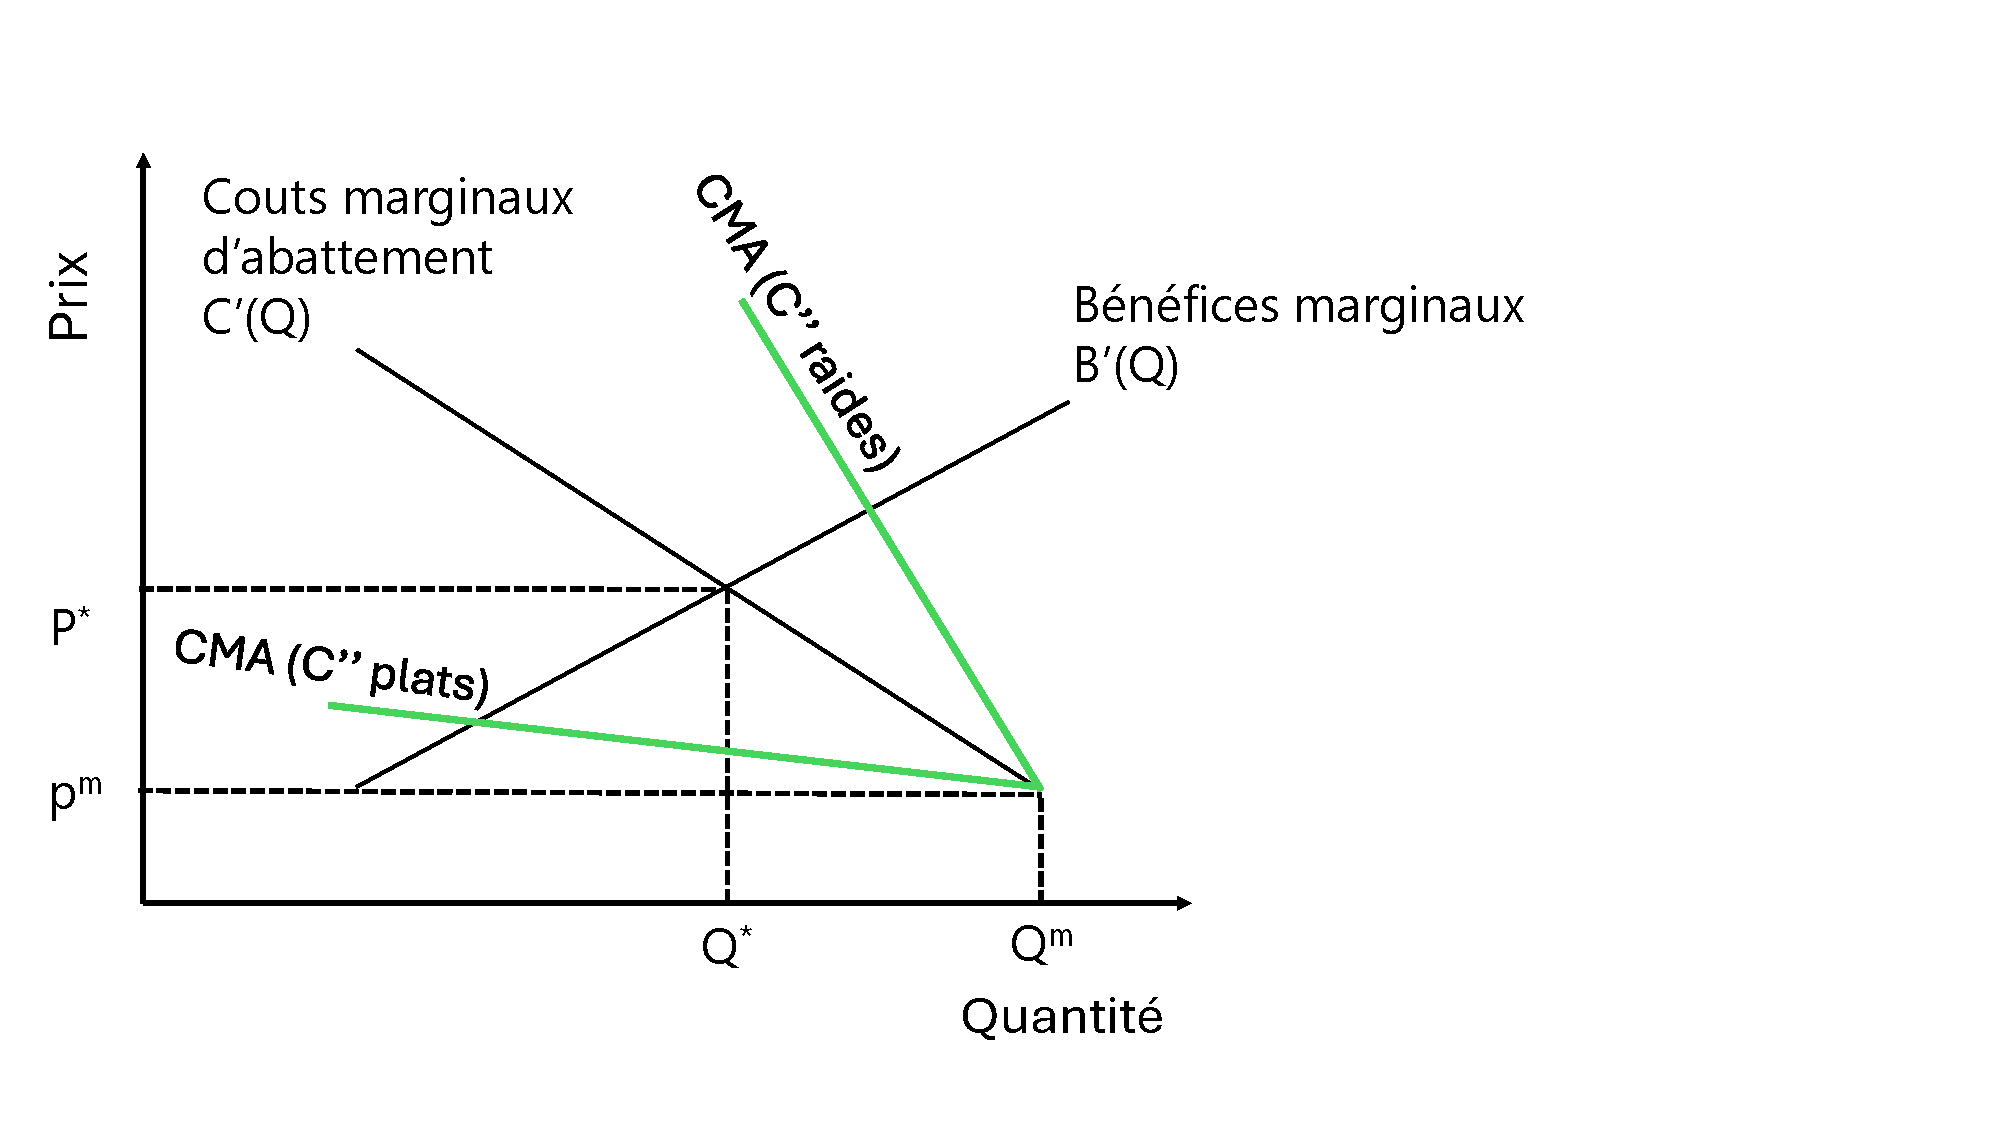
\includegraphics[width=1.1\textwidth]{mac_md_curves/md_bma_plats.pdf}
% % }

% % \end{frame}


% \begin{frame}{Taxe vs quota : curbe DM plate}

% \centering
% \begin{tikzpicture}[scale=1.2]

% % Paramètres (MD relativement plat)
% \pgfmathsetmacro{\m}{0.6}
% \pgfmathsetmacro{\bE}{0.2}
% \pgfmathsetmacro{\bA}{1.2}
% \pgfmathsetmacro{\k}{3.2}
% \pgfmathsetmacro{\d}{0.2} % MD plat

% % Point de pivot : intersection CMAr et DM
% \pgfmathsetmacro{\Rpivot}{(\k-\bE)/(\m+\d)}
% \pgfmathsetmacro{\tlevel}{\m*\Rpivot+\bE}  % taxe passe par CMAr au pivot

% % Points clés
% \pgfmathsetmacro{\Ro}{(\k-\bA)/(\m+\d)}
% \pgfmathsetmacro{\yRo}{\m*\Ro+\bA}

% \pgfmathsetmacro{\Rq}{(\k-\bE)/(\m+\d)}
% \pgfmathsetmacro{\yRq}{\m*\Rq+\bE}

% % Rt : intersection CMA* et taxe
% \pgfmathsetmacro{\Rt}{(\tlevel-\bA)/\m}
% \pgfmathsetmacro{\yMDatRt}{\k-\d*\Rt}

% \pgfmathsetmacro{\Cq}{\m*\Rq+\bA}

% % Axes
% \draw[->, thick] (0,0) -- (6,0) node[below] {Réduction de la pollution};
% \draw[->, thick] (0,0) -- (0,5.3) node[above] {Coût / Dommage};

% % Courbes
% \draw[thick, blue, dotted] (0.5, {\m*0.5+\bA}) -- (6.8, {\m*6.8+\bA});
% \node[blue] at (6.75, {\m*7.2+\bA}) {$CMA^*$};

% \draw[thick, blue] (0.5, {\m*0.5+\bE}) -- (6.8, {\m*6.8+\bE});
% \node[blue] at (6.75, {\m*7.2+\bE}) {$CMA_r$};

% \draw[thick, red] (0.5, {\k-\d*0.5}) -- (6.8, {\k-\d*6.8});
% \node[red] at (7.5, {\k-\d*6.8}) {$DM (B'')$};

% % Taxe (passe maintenant par l'intersection CMAr-DM)
% \draw[thick, green!70!black] (0.5,\tlevel) -- (6.8,\tlevel);
% \node[left] at (0,\tlevel) {$t=C_t$};

% % Verticales
% \draw[dashed] (\Rt,0) -- (\Rt,\yMDatRt);
% \node[below] at (\Rt,0) {$R_t$};

% \draw[dashed] (\Ro,0) -- (\Ro,\yRo);
% \node[below] at (\Ro,0) {$R^{o}$};

% \draw[dashed] (\Rq,0) -- (\Rq,\Cq);
% \node[below] at (\Rq,0) {$R_q$};

% % Horizontale Cq
% \draw[dashed] (0,\Cq) -- (\Rq,\Cq);
% \node[left] at (0,\Cq) {$C_q$};

% % DWL taxe
% \fill[green!60, opacity=0.55]
% (\Rt,\tlevel) -- (\Ro,\yRo) -- (\Rt,\yMDatRt) -- cycle;
% \node at ({(\Rt+\Ro)/2 -0.1}, {\tlevel+0.6}) {$DWL_t$};

% % DWL quota
% \fill[yellow, opacity=0.55]
% (\Ro,\yRo) -- (\Rq,\yRq) -- (\Rq,\Cq) -- cycle;
% \node at ({(\Ro+\Rq)/2 +0.15}, {\yRo+0.95}) {$DWL_q$};

% \end{tikzpicture}

% \end{frame}


% \begin{frame}{Taxe vs quota : curbe DM raide}
% \centering
% \begin{tikzpicture}[scale=1.2]
% % Paramètres
% \pgfmathsetmacro{\m}{0.6}        % pente des CMA
% \pgfmathsetmacro{\bE}{0.2}       % intercept CMAr
% \pgfmathsetmacro{\bA}{1.2}       % intercept CMA*

% % Point de pivot fixe : intersection CMAr et taxe
% % On choisit Rt = 2.5 comme point de pivot
% \pgfmathsetmacro{\Rpivot}{2.5}
% \pgfmathsetmacro{\tlevel}{\m*\Rpivot+\bE}  % taxe passe par CMAr au pivot

% % Nouvelle pente pour DM (beaucoup plus pentu)
% \pgfmathsetmacro{\d}{1.2}

% % Recalculer k pour que MD passe par le point de pivot (Rpivot, tlevel)
% \pgfmathsetmacro{\k}{\tlevel + \d*\Rpivot}

% % Points clés
% % R* (optimal) : intersection CMA* et MD
% \pgfmathsetmacro{\Ro}{(\k-\bA)/(\m+\d)}
% \pgfmathsetmacro{\yRo}{\m*\Ro+\bA}

% % Rt : intersection CMA* et taxe (à gauche de R*)
% \pgfmathsetmacro{\Rt}{(\tlevel-\bA)/\m}
% \pgfmathsetmacro{\yMDatRt}{\k-\d*\Rt}

% % Rq : intersection CMAr et MD (à droite de R*)
% \pgfmathsetmacro{\Rq}{(\k-\bE)/(\m+\d)}
% \pgfmathsetmacro{\yRq}{\m*\Rq+\bE}
% \pgfmathsetmacro{\Cq}{\m*\Rq+\bA}  % coût sur CMA* à Rq

% % Axes
% \draw[->, thick] (0,0) -- (6,0) node[below] {Réduction de la pollution};
% \draw[->, thick] (0,0) -- (0,5.3) node[above] {Coût / Dommage};

% % Courbe CMA* (bleu pointillé)
% \draw[thick, blue, dotted] (0.5, {\m*0.5+\bA}) -- (6.8, {\m*6.8+\bA});
% \node[blue] at (6.75, {\m*7.2+\bA}) {$CMA^*$};

% \draw[thick, blue] (0.3, {\m*0.3+\bE}) -- (5.2, {\m*5.2+\bE});
% \node[blue] at (5.8, {\m*5.2+\bE}) {$CMA_r$};

% % Courbe DM (pente négative forte)
% \draw[thick, red] (0.3, {\k-\d*0.3}) -- (3.8, {\k-\d*3.8});
% \node[red] at (4.5, {\k-\d*3.8+0.1}) {$DM (B'')$};

% % Taxe (horizontale passant par le pivot)
% \draw[thick, green!70!black] (0.3,\tlevel) -- (5.2,\tlevel);
% \node[left] at (0,\tlevel) {$t=C_t$};

% % Verticales
% \draw[dashed] (\Rt,0) -- (\Rt,\yMDatRt);
% \node[below] at (\Rt,0) {$R_t$};

% \draw[dashed] (\Ro,0) -- (\Ro,\yRo);
% \node[below] at (\Ro,0) {$R^{o}$};

% \draw[dashed] (\Rq,0) -- (\Rq,\Cq);
% \node[below] at (\Rq,0) {$R_q$};

% % Horizontale Cq
% \draw[dashed] (0,\Cq) -- (\Rq,\Cq);
% \node[left] at (0,\Cq) {$C_q$};

% % DWL taxe : triangle entre Rt, R* sur les courbes
% \fill[green!60, opacity=0.55]
%   (\Rt,\tlevel) -- (\Ro,\yRo) -- (\Rt,\yMDatRt) -- cycle;
% \node at ({(\Rt+\Ro)/2}, {(\tlevel+\yMDatRt)/2.4 + 0.75}) {$DWL_t$};

% % DWL quota : triangle entre R*, Rq
% \fill[yellow, opacity=0.55]
%   (\Ro,\yRo) -- (\Rq,\yRq) -- (\Rq,\Cq) -- cycle;
% \node at ({(\Ro+\Rq)/2 + 0.9}, {\yRo+0.1}) {$DWL_q$};

% \end{tikzpicture}
% \end{frame}



% %========================
% % Slide: Contingency table MAC vs MD
% %========================
% \begin{frame}{Prix ou quantité ? Rôle de la courbure des courbes}

% \centering
% \renewcommand{\arraystretch}{1.8} % plus d'espace vertical
% \begin{tabular}{>{\centering\arraybackslash}m{3cm}|>{\centering\arraybackslash}m{3.5cm}|>{\centering\arraybackslash}m{3.5cm}}
% \toprule
%  & \textbf{CMA plats} \newline \small{($C''$ faible)} & \textbf{CMA raides} \newline \small{($C''$ élevé)} \\
% \midrule
% \textbf{DM plats} \newline \small{($|B''|$ faible)} 
% & \cellcolor{gray!20} Instruments équivalents 
% & \cellcolor{green!25} \textbf{Prix préférables} \\
% \midrule
% \textbf{DM raides} \newline \small{($|B''|$ élevé)} 
% & \cellcolor{yellow!35} \textbf{Quantités préférables} 
% & \cellcolor{gray!20} Instruments équivalents \\
% \bottomrule
% \end{tabular}

% \vspace{0.5cm}

% \begin{itemize}
%   \item DM raides : erreurs de pollution très coûteuses $\Rightarrow$ quantités.
%   \item CMA raides : erreurs de coûts très coûteuses $\Rightarrow$ prix.
% \end{itemize}

% \end{frame}


% \begin{frame}{Conclusion : Prix vs Quantité}

% \textbf{Résultat clé (Weitzman 1974)}
% \begin{itemize}
%     \item Régulation par les \textbf{prix} ou les \textbf{quantités} en fonction de la relation  $CMA'$ vs $ DM'$
% \end{itemize}

% \vspace{0.4cm}
% \textbf{Limitation liées aux hypothèses sous-jacentes}
% \begin{enumerate}
%     \item \textbf{Hétérogénéité des firmes} : Un quota sans marché de permis devient plus inefficace avec des CMA hétérogènes.
    
%     \item \textbf{Non-linéarité des dommages} : L'hypothèse de linéarité est questionnable face aux points de basculement climatiques ('tipping points') et une potentielle irreversibilité $\Rightarrow$ favorise la régulation par quantités.

% \end{enumerate}

% \vspace{0.4cm}
% \textbf{Conclusion :} Pas de jugement définitif sur la supériorité d'un instrument, mais un cadre utile pour comprendre les arbitrages.

% \end{frame}



% \subsection{Growth models}

% % Slide 1: Output as function of labor
% \begin{frame}[plain,label=growth1]
%   \Large
%   \[
%     Y = L
%   \]
%   \vspace{1em}
%   \begin{itemize}\Large
%     \item $Y$: output (GDP)
%     \item $L$: labor (population)
%   \end{itemize}
% \end{frame}

% % Slide 2: Include capital
% \begin{frame}[plain,label=growth2]
%   \Large
%   \[
%     Y = K \times L
%   \]
%   \vspace{1em}
%   \begin{itemize}\Large
%     \item $Y$: output (GDP)
%     \item $L$: labor (population)
%     \item $K$: capital (machines)
%   \end{itemize}
% \end{frame}

% % Slide 3: Include technology
% \begin{frame}[plain,label=growth3]
%   \Large
%   \[
%     Y = A \times K \times L
%   \]
%   \vspace{1em}
%   \begin{itemize}\Large
%     \item $Y$: output (GDP)
%     \item $L$: labor (population)
%     \item $K$: capital (machines)
%     \item $A$: technology (exogenous)
%   \end{itemize}
% \end{frame}

% % Slide 4: Production & Savings → Investment
% \begin{frame}[plain,label=growth4]
%   \Large

%   % Equation (1)
%   \[
%     \tag{1}\;Y = A \times K \times L
%   \]

%   \vspace{1em}

%   % Equation (2)
%   \[
%     \tag{2}\;s \times Y = I = \Delta K
%   \]
%   \vspace{0.5em}
%   \begin{itemize}\Large
%     \item $s$: savings rate (fraction of output saved)
%     \item $sY$: saved (unconsumed) output
%     \item $I$: investment
%     \item $\Delta K$: change in capital stock (new investment)
%   \end{itemize}
% \end{frame}

% % Slide: Endogenizing Technology (A)
% \begin{frame}[plain,label=growth5]
%   \Large
%   \[
%     \tag{1}\;Y = A(t)\,\;K^\alpha\,L^{1-\alpha}
%   \]
%   \vspace{0.75em}
%   \[
%     \tag{2}\;\dot A = \underbrace{\phi\,A^\lambda\,L_A}_{\text{R\&D production}}\quad\Longrightarrow\quad
%     \text{A grows without bound.}
%   \]
%   \vspace{0.5em}
%   \begin{itemize}\Large
%     \item In Solow: \(A\) exogenous, fixed  
%     \item {\bf Romer (1990)}: \(\dot A=\phi\,A\,L_A\) (non-rival spillovers) 
%     \item {\bf Lucas (1988)}: human-capital externality, \(\dot H = \psi\,H\,u_H\) with \(u_H\) in R\&D 
%     \item {\bf Aghion–Howitt (1992)}: creative destruction, \(\dot A = \mu\,\bigl(\tfrac{K_R}{\bar K}\bigr)^\eta A\) from innovation races  
%     \item Knowledge accumulation → perpetual, scale‐sensitive growth
%   \end{itemize}
% \end{frame}

% \subsection{NPV, discount rate, LCOE}

% \begin{frame}[label=nb1]{Net Benefits (Undiscounted)}

% \textbf{Approach 1: Sum of Benefits minus Sum of Costs}
% \[
% NB = \left(\sum_{t=0}^{N} B_t\right) - \left(\sum_{t=0}^{N} C_t\right)
% \]

% \textbf{Approach 2: Sum of Net Benefits per Period}
% \[
% NB = \sum_{t=0}^{N} (B_t - C_t)
% \]

% \vspace{0.5cm}

% \textbf{Three-Period Example (t = 0 to t = 2):}

% \textbf{Approach 1:}
% \[
% NB = (B_0 + B_1 + B_2) - (C_0 + C_1 + C_2)
% \]

% \textbf{Approach 2:}
% \[
% NB = (B_0 - C_0) + (B_1 - C_1) + (B_2 - C_2)
% \]

% \end{frame}

% \begin{frame}[label=npv1]{Net Present Value (Discounted)}

% \textbf{Approach 1: PV of Benefits minus PV of Costs}
% \[
% NPV = \left(\sum_{t=0}^{N} \frac{B_t}{(1+r)^t}\right) - \left(\sum_{t=0}^{N} \frac{C_t}{(1+r)^t}\right)
% \]

% \textbf{Approach 2: Sum of Discounted Net Benefits}
% \[
% NPV = \sum_{t=0}^{N} \frac{(B_t - C_t)}{(1+r)^t}
% \]

% \vspace{0.5cm}

% \textbf{Three-Period Example (t = 0 to t = 2):}

% \textbf{Approach 1:}
% \[
% NPV = \left(B_0 + \frac{B_1}{(1+r)} + \frac{B_2}{(1+r)^2}\right) - \left(C_0 + \frac{C_1}{(1+r)} + \frac{C_2}{(1+r)^2}\right)
% \]

% \textbf{Approach 2:}
% \[
% NPV = (B_0 - C_0) + \frac{(B_1 - C_1)}{(1+r)} + \frac{(B_2 - C_2)}{(1+r)^2}
% \]

% \end{frame}


% \begin{frame}[label=discount1]{Discount Rates: Different Perspectives}

% \textbf{The Discount Factor:}
% \[
% d_t = \frac{1}{(1+r)^t}
% \]

% \vspace{0.3cm}

% \textbf{Three Cases:}

% \begin{itemize}
%     \item \textbf{$r \rightarrow 0$ (Environmentalist/Ethical Case):} Present and future benefits/costs are equally weighted. Intergenerational equity: future generations matter as much as current generation.
    
%     \item \textbf{$r > 0$ (Economist Case):} Preference for the present, reflecting opportunity costs and time preference.
%     \begin{itemize}
%         \item Stern Review: $r \approx 1.4\%$ (low pure time preference)
%         \item Nordhaus: $r \approx 4.5\%$ (market-based approach)
%     \end{itemize}
    
%     \item \textbf{$r < 0$ (Theoretical Case):} Future benefits and costs weighted higher than present. Not used in practice but conceptually relevant for growing environmental damages.
% \end{itemize}

% \end{frame}

% \begin{frame}[label=discount2]{Discount Rates: Example}

% \textbf{Project with net benefit of \$1,000,000 received in 30 years}

% \textbf{NPV calculation:}
% \[
% NPV = \frac{1,000,000}{(1+r)^{30}}
% \]

% \vspace{0.3cm}

% \begin{table}[]
% \centering
% \begin{tabular}{lcc}
% \hline
% \textbf{Perspective} & \textbf{Discount Rate} & \textbf{NPV (\$)} \\
% \hline
% Environmentalist & $r = 0\%$ & 1,000,000 \\
% Stern (Climate) & $r = 1.4\%$ & 659,000 \\
% EPA/Social & $r = 3\%$ & 412,000 \\
% Nordhaus & $r = 4.5\%$ & 267,000 \\
% Private/Market & $r = 7\%$ & 131,000 \\
% High Private & $r = 10\%$ & 57,000 \\
% \hline
% \end{tabular}
% \end{table}

% \vspace{0.2cm}
% \small{Choice of discount rate dramatically affects project valuation!}

% \end{frame}

% \begin{frame}[label=lcoe1]{Levelized Cost of Energy (LCOE) - Private Costs}

% \textbf{Standard LCOE Formula (Private Costs Only):}
% \[
% LCOE = \frac{\sum_{t=0}^{N} \frac{I_t + M_t + F_t}{(1+r)^t}}{\sum_{t=0}^{N} \frac{E_t}{(1+r)^t}}
% \]

% \vspace{0.3cm}

% \textbf{Components:}
% \begin{itemize}
%     \item $I_t$ = Capital investment costs in year $t$ (construction, equipment)
%     \item $M_t$ = Operations \& maintenance costs in year $t$ (labor, repairs)
%     \item $F_t$ = Fuel costs in year $t$ (coal, gas, uranium; \$0 for renewables)
%     \item $E_t$ = Electricity generated in year $t$ (MWh)
%     \item $r$ = Discount rate (cost of capital)
%     \item $N$ = Project lifetime (typically 20-40 years)
% \end{itemize}

% \vspace{0.2cm}
% \textbf{Units:} Typically expressed in \$/MWh or \$/kWh

% \end{frame}

% \begin{frame}[label=lcoe2]{LCOE with External Costs}

% \textbf{Social LCOE Formula (Including Carbon Price):}
% \[
% LCOE_{social} = \frac{\sum_{t=0}^{N} \frac{I_t + M_t + F_t + (CO2_t \times P_{carbon,t})}{(1+r)^t}}{\sum_{t=0}^{N} \frac{E_t}{(1+r)^t}}
% \]

% \vspace{0.3cm}

% \textbf{Additional Components:}
% \begin{itemize}
%     \item $CO2_t$ = CO$_2$ emissions in year $t$ (tons)
%     \item $P_{carbon,t}$ = Carbon price in year $t$ (\$/ton CO$_2$)
%     \item Captures climate externality costs
% \end{itemize}

% \vspace{0.2cm}
% \textbf{Note:} For comprehensive social LCOE, would also add health damages (PM$_{2.5}$, NO$_x$, SO$_2$), water use, land degradation, etc.

% \end{frame}

% \begin{frame}[label=lcoe3]{LCOE Example: Three-Period Case}

% \textbf{Assumptions:} Coal plant, $r = 7\%$, 3 years (simplified)

% \textbf{Without External Costs:}
% \[
% LCOE_{private} = \frac{1000 + \frac{50+30+40}{1.07} + \frac{50+30+40}{1.07^2}}{1000 + \frac{1000}{1.07} + \frac{1000}{1.07^2}}
% \]
% \[
% = \frac{1000 + 112.1 + 104.8}{1000 + 934.6 + 873.4} = \frac{1216.9}{2808.0} = \$0.43/\text{MWh-unit}
% \]

% \vspace{0.3cm}

% \textbf{With External Costs (Carbon Price = \$50/ton, 1 ton CO$_2$/MWh):}
% \[
% LCOE_{social} = \frac{1000 + \frac{50+30+40+50}{1.07} + \frac{50+30+40+50}{1.07^2}}{1000 + \frac{1000}{1.07} + \frac{1000}{1.07^2}}
% \]
% \[
% = \frac{1000 + 158.9 + 148.5}{2808.0} = \frac{1307.4}{2808.0} = \$0.47/\text{MWh-unit}
% \]

% \small{External costs increase LCOE by $\sim$9\% in this example}

% \end{frame}

% \begin{frame}[label=lcoe4]{LCOE Example: Detailed Breakdown}

% \textbf{Three-Period Example Details:}

% \vspace{0.3cm}

% \begin{table}[]
% \centering
% \small
% \begin{tabular}{lcccc}
% \hline
% \textbf{Period} & \textbf{$I_t$} & \textbf{$M_t$} & \textbf{$F_t$} & \textbf{$E_t$} \\
% \hline
% $t=0$ & 1000 & 0 & 0 & 1000 MWh \\
% $t=1$ & 0 & 50 & 30+40=70 & 1000 MWh \\
% $t=2$ & 0 & 50 & 30+40=70 & 1000 MWh \\
% \hline
% \end{tabular}
% \end{table}

% \vspace{0.3cm}

% \textbf{Carbon Externality:}
% \begin{itemize}
%     \item Coal emissions: 1 ton CO$_2$ per MWh
%     \item Carbon price: \$50/ton
%     \item Annual external cost: 1000 MWh $\times$ 1 ton/MWh $\times$ \$50/ton = \$50
% \end{itemize}

% \vspace{0.2cm}

% \textbf{Key Insight:} Renewable energy (solar/wind) has $F_t = 0$ and $CO2_t = 0$, making social LCOE $\approx$ private LCOE

% \end{frame}

% \begin{frame}[label=altdisc1]{Alternative Discount Rate Approaches for Environmental Costs}

% \textbf{The Problem:} Standard discounting may undervalue environmental damages because:
% \begin{itemize}
%     \item Irreversible damages (extinction, ecosystem collapse)
%     \item Intergenerational equity concerns
%     \item Growing marginal damages over time
%     \item Non-substitutability of natural capital
% \end{itemize}

% \vspace{0.3cm}

% \textbf{Three Alternative Approaches:}
% \begin{enumerate}
%     \item Dual/Differential Discounting
%     \item Declining Discount Rates
%     \item Shadow Price with Growing Damages
% \end{enumerate}

% \end{frame}

% \begin{frame}[label=dual1]{Option 1: Dual/Differential Discounting}

% \textbf{Concept:} Use different discount rates for different types of impacts

% \[
% NPV = \sum_{t=0}^{N} \frac{B_t}{(1+r_{financial})^t} - \sum_{t=0}^{N} \frac{C_t}{(1+r_{financial})^t} - \sum_{t=0}^{N} \frac{D_t^{env}}{(1+r_{environmental})^t}
% \]

% Where: $r_{financial} > r_{environmental}$

% \vspace{0.3cm}

% \textbf{Typical Values:}
% \begin{itemize}
%     \item Financial costs/benefits: $r = 3-7\%$
%     \item Environmental damages: $r = 0-2\%$
% \end{itemize}

% \vspace{0.3cm}

% \textbf{Rationale:} Environmental goods become relatively scarcer over time; low substitutability with market goods; ethical obligations to future generations

% \end{frame}

% \begin{frame}[label=dual2]{Dual Discounting: Key References}

% \textbf{Foundational Papers:}

% \begin{itemize}
%     \small
%     \item \textbf{Weitzman, M.L. (1994).} "On the 'Environmental' Discount Rate." \textit{Journal of Environmental Economics and Management}, 26(2), 200-209.
    
%     \item \textbf{Gollier, C. (2010).} "Ecological discounting." \textit{Journal of Economic Theory}, 145(2), 812-829.
    
%     \item \textbf{Hoel, M. \& Sterner, T. (2007).} "Discounting and relative prices." \textit{Climatic Change}, 84(3-4), 265-280.
    
%     \item \textbf{Traeger, C.P. (2011).} "Sustainability, limited substitutability, and non-constant social discount rates." \textit{Journal of Environmental Economics and Management}, 62(2), 215-228.
    
%     \item \textbf{Weikard, H.P. \& Zhu, X. (2005).} "Discounting and environmental quality: When should dual rates be used?" \textit{Economic Modelling}, 22(5), 868-878.
    
%     \item \textbf{Baumgärtner, S. et al. (2015).} "Trade-offs between justices and efficiency." \textit{Environmental and Resource Economics}, 60, 97-118.
% \end{itemize}

% \end{frame}

% \begin{frame}[label=ddr1]{Option 2: Declining Discount Rates (DDR)}

% \textbf{Concept:} Discount rate decreases over time horizon

% \[
% NPV = \sum_{t=0}^{N} \frac{(B_t - C_t)}{(1+r_t)^t}
% \]

% Where: $r_t = r_0 \cdot e^{-\gamma t}$ or use step function

% \vspace{0.3cm}

% \textbf{Example (UK Green Book):}
% \begin{table}[]
% \small
% \begin{tabular}{ll}
% \hline
% \textbf{Time Period} & \textbf{Discount Rate} \\
% \hline
% Years 0-30 & 3.5\% \\
% Years 31-75 & 3.0\% \\
% Years 76-125 & 2.5\% \\
% Years 126-200 & 2.0\% \\
% Years 201-300 & 1.5\% \\
% Years 301+ & 1.0\% \\
% \hline
% \end{tabular}
% \end{table}

% \vspace{0.2cm}

% \textbf{Rationale:} Uncertainty about future discount rates; precautionary principle; intergenerational equity

% \end{frame}

% \begin{frame}[label=ddr2]{Declining Discount Rates: Key References}

% \textbf{Foundational Papers:}

% \begin{itemize}
%     \small
%     \item \textbf{Weitzman, M.L. (1998).} "Why the far-distant future should be discounted at its lowest possible rate." \textit{Journal of Environmental Economics and Management}, 36(3), 201-208.
    
%     \item \textbf{Weitzman, M.L. (2001).} "Gamma discounting." \textit{American Economic Review}, 91(1), 260-271.
    
%     \item \textbf{Gollier, C. (2002).} "Time horizon and the discount rate." \textit{Journal of Economic Theory}, 107(2), 463-473.
    
%     \item \textbf{Newell, R.G. \& Pizer, W.A. (2003).} "Discounting the distant future: how much do uncertain rates increase valuations?" \textit{Journal of Environmental Economics and Management}, 46(1), 52-71.
    
%     \item \textbf{Arrow, K.J. et al. (2013).} "Determining benefits and costs for future generations." \textit{Science}, 341(6144), 349-350.
    
%     \item \textbf{Groom, B. et al. (2005).} "Declining discount rates: the long and the short of it." \textit{Environmental and Resource Economics}, 32(4), 445-493.
% \end{itemize}

% \end{frame}

% \begin{frame}[label=shadow1]{Option 3: Shadow Price with Growing Marginal Damages}

% \textbf{Concept:} Don't discount damages directly; discount shadow price of carbon which accounts for growing damages

% \[
% SCC_t = \sum_{s=t}^{N} \frac{MD_s(Stock_s)}{(1+r)^{s-t}}
% \]

% Where:
% \begin{itemize}
%     \item $MD_s$ = Marginal damage at time $s$ (depends on cumulative stock)
%     \item $Stock_s$ = $Stock_{s-1} + Emissions_s - Decay_s$
%     \item Damages grow non-linearly as stock accumulates
% \end{itemize}

% \vspace{0.3cm}

% \textbf{Key insight:} Even with positive $r$, if $MD_s$ grows faster than discount rate, present value of future damages increases

% \textbf{Example:} US Government Social Cost of Carbon
% \begin{itemize}
%     \item 2020: \$51/ton CO$_2$ → 2050: \$85/ton (real terms, at 3\% discount)
% \end{itemize}

% \end{frame}

% \begin{frame}[label=shadow2]{Shadow Price Approach: Key References}

% \textbf{Foundational Papers:}

% \begin{itemize}
%     \small
%     \item \textbf{Interagency Working Group (2021).} "Technical Support Document: Social Cost of Carbon, Methane, and Nitrous Oxide." US Government.
    
%     \item \textbf{Dietz, S. \& Stern, N. (2015).} "Endogenous growth, convexity of damage and climate risk: How Nordhaus' framework supports deep cuts in carbon emissions." \textit{Economic Journal}, 125(583), 574-620.
    
%     \item \textbf{Pindyck, R.S. (2013).} "Climate change policy: What do the models tell us?" \textit{Journal of Economic Literature}, 51(3), 860-872.
    
%     \item \textbf{National Academies (2017).} \textit{Valuing Climate Damages: Updating Estimation of the Social Cost of Carbon Dioxide.} Washington, DC: National Academies Press.
    
%     \item \textbf{Rennert, K. et al. (2022).} "Comprehensive evidence implies a higher social cost of CO$_2$." \textit{Nature}, 610, 687-692.
% \end{itemize}

% \vspace{0.2cm}

% \textbf{Policy Documents:}
% \begin{itemize}
%     \small
%     \item UK HM Treasury Green Book (2022)
%     \item World Bank Shadow Price of Carbon Guidance (2024)
% \end{itemize}

% \end{frame}

% \begin{frame}[label=comparison]{Comparison of Three Approaches}

% \begin{table}[]
% \tiny
% \begin{tabular}{p{2cm}p{3cm}p{3cm}p{3cm}}
% \hline
% \textbf{Approach} & \textbf{Mechanism} & \textbf{Advantages} & \textbf{Challenges} \\
% \hline
% \textbf{Dual Rates} & Different $r$ for environmental vs. financial & Simple; reflects scarcity; ethical foundation & Theoretically contentious; arbitrary rate selection \\
% \hline
% \textbf{Declining Rates} & $r_t$ decreases over time & Captures uncertainty; UK/France adopted & Time inconsistency issues; complex implementation \\
% \hline
% \textbf{Shadow Price} & Damages grow in numerator & Theoretically consistent; used by US govt & Requires damage function modeling; high uncertainty \\
% \hline
% \end{tabular}
% \end{table}

% \vspace{0.3cm}

% \textbf{Common Thread:} All three approaches give greater weight to distant future environmental damages than standard constant discounting at market rates (3-7\%)

% \vspace{0.2cm}

% \textbf{Policy Adoption:}
% \begin{itemize}
%     \item UK: Declining rates (Green Book)
%     \item US: Shadow price approach (SCC)
%     \item France: Combination of approaches
%     \item World Bank: Shadow price guidance for client countries
% \end{itemize}

% \end{frame}

% \subsection{Cap and Trade System: Part A}

% \begin{frame}{Setting up the System of Equations}

% We have two equations with two unknowns ($Q_A$ and $Q_B$):

% \vspace{0.5cm}

% \textbf{Equation 1 (Total abatement constraint):}
% \begin{equation}
% Q_A + Q_B = 50
% \end{equation}

% \vspace{0.5cm}

% \textbf{Equation 2 (Equal MAC condition):}
% \begin{equation}
% 2Q_A + 0.5Q_A^2 = Q_B + 0.2Q_B^2
% \end{equation}
% \end{frame}

% \begin{frame}{Solving the System: Steps 1-2}

% \textbf{Step 1: Express $Q_A$ in terms of $Q_B$}

% From Equation 1:
% \begin{equation}
% Q_A = 50 - Q_B
% \end{equation}

% \vspace{0.5cm}

% \textbf{Step 2: Substitute into Equation 2}

% \begin{equation}
% 2(50 - Q_B) + 0.5(50 - Q_B)^2 = Q_B + 0.2Q_B^2
% \end{equation}

% \end{frame}

% \begin{frame}{Mathematical Tools and Expansion}
% \textbf{Algebraic Identities:}
% \begin{align}
% (a + b)^2 &= a^2 + 2ab + b^2 \\
% (a - b)^2 &= a^2 - 2ab + b^2
% \end{align}
% \vspace{0.3cm}
% \textbf{Quadratic Formula:}
% \begin{equation}
% \text{For } ax^2 + bx + c = 0, \quad x = \frac{-b \pm \sqrt{b^2 - 4ac}}{2a}
% \end{equation}
% \end{frame}


% \begin{frame}{Mathematical Tools and Expansion}

% \textbf{Algebraic Identities:}
% \begin{align}
% (a + b)^2 &= a^2 + 2ab + b^2 \\
% (a - b)^2 &= a^2 - 2ab + b^2
% \end{align}

% \textit{Example from our problem:}
% $$(50 - Q_B)^2 = 50^2 - 2(50)(Q_B) + Q_B^2 = 2500 - 100Q_B + Q_B^2$$

% \vspace{0.3cm}

% \textbf{Quadratic Formula:}
% \begin{equation}
% \text{For } ax^2 + bx + c = 0, \quad x = \frac{-b \pm \sqrt{b^2 - 4ac}}{2a}
% \end{equation}

% \textit{Example from our problem:}
% $$0.3Q_B^2 - 53Q_B + 1350 = 0$$
% $$\text{where } a = 0.3, \; b = -53, \; c = 1350$$

% \end{frame}

% \begin{frame}{Step 3: Expand the Binomial Term}

% \textbf{Starting equation:}
% $$2(50 - Q_B) + \colorbox{red!30}{$0.5(50 - Q_B)^2$} = Q_B + 0.2Q_B^2$$

% \vspace{0.2cm}

% \textbf{Algebraic Identities:}
% \begin{align}
% (a + b)^2 &= a^2 + 2ab + b^2 \\
% (a - b)^2 &= a^2 - 2ab + b^2
% \end{align}

% \vspace{0.2cm}

% \textbf{Solve the identity term } $\colorbox{red!30}{$(50 - Q_B)^2$}$:
% \begin{align}
% (50 - Q_B)^2 &= 50^2 - 2(50)(Q_B) + Q_B^2 \\
% &= 2500 - 100Q_B + Q_B^2
% \end{align}

% Therefore:
% \begin{align}
% 0.5(50 - Q_B)^2 &= 0.5(2500 - 100Q_B + Q_B^2) \\
% &= 1250 - 50Q_B + 0.5Q_B^2
% \end{align}

% \end{frame}

% \begin{frame}{Step 4: Substitute and Rearrange}

% \textbf{Original equation:}
% $$2(50 - Q_B) + \colorbox{red!30}{$0.5(50 - Q_B)^2$} = Q_B + 0.2Q_B^2$$

% \vspace{0.3cm}

% \textbf{Substitute the expanded term:}
% $$100 - 2Q_B + \colorbox{red!30}{$1250 - 50Q_B + 0.5Q_B^2$} = Q_B + 0.2Q_B^2$$

% \vspace{0.3cm}

% \textbf{Rearrange to standard quadratic form } $ax^2 + bx + c = 0$:
% $$0.3Q_B^2 - 53Q_B + 1350 = 0$$

% \end{frame}


% \begin{frame}{Step 5: Using Quadratic Formula to Calculate $Q_B^*$}

% \textbf{Quadratic equation:}
% $$0.3Q_B^2 - 53Q_B + 1350 = 0$$

% where $a = 0.3$, $b = -53$, $c = 1350$

% \vspace{0.3cm}

% \textbf{Apply quadratic formula:}
% $$Q_B = \frac{-b \pm \sqrt{b^2 - 4ac}}{2a} = \frac{-(-53) \pm \sqrt{(-53)^2 - 4(0.3)(1350)}}{2(0.3)}$$

% $$Q_B = \frac{53 \pm \sqrt{2809 - 1620}}{0.6} = \frac{53 \pm \sqrt{1189}}{0.6}$$

% $$Q_B = \frac{53 \pm 34.48}{0.6}$$

% \textbf{Two solutions:}
% $$Q_B = \frac{53 + 34.48}{0.6} = 145.8 \quad \text{or} \quad Q_B^* = \frac{53 - 34.48}{0.6} = 30.87 \text{ tons}$$

% \end{frame}




% \begin{frame}{Step 6: Using Optimal $Q_B^*$ to Get $Q_A^*$}

% \textbf{From the constraint equation:}
% $$Q_A + Q_B = 50$$

% \vspace{0.3cm}

% \textbf{Substitute } $Q_B^* = 30.87$ tons:
% $$Q_A^* = 50 - Q_B^*$$

% $$Q_A^* = 50 - 30.87$$

% $$Q_A^* = 19.13 \text{ tons}$$

% \end{frame}

% \begin{frame}{Step 7: Using MAC to Calculate $P^*$}

% \textbf{Using Plant B's MAC equation:}
% $$P^* = Q_B + 0.2Q_B^2 = 30.87 + 0.2(30.87)^2$$

% $$P^* = 30.87 + 0.2(952.96) = 30.87 + 190.59$$

% $$P^* = \$221.46 \text{ per ton}$$

% \vspace{0.5cm}

% \textbf{Verification using Plant A's MAC equation:}
% $$P^* = 2Q_A + 0.5Q_A^2 = 2(19.13) + 0.5(19.13)^2$$

% $$P^* = 38.26 + 0.5(365.96) = 38.26 + 182.98$$

% $$P^* = \$221.24 \text{ per ton} \quad \checkmark$$

% \end{frame}


% \begin{frame}{Step 8: Permits and Emission Levels}

% \textbf{Initial permit allocation (50 tons each):}
% \begin{itemize}
%     \item Plant A (Coal): 50 tons
%     \item Plant B (Gas): 50 tons
%     \item Total: 100 tons
% \end{itemize}

% \vspace{0.3cm}

% \textbf{Actual emissions after abatement:}
% \begin{align}
% \text{Plant A (Coal) emissions} &= \text{Baseline} - Q_A^* = 100 - 19.13 = 80.87 \text{ tons} \\
% \text{Plant B (Gas) emissions} &= \text{Baseline} - Q_B^* = 50 - 30.87 = 19.13 \text{ tons}
% \end{align}

% \vspace{0.3cm}

% \textbf{Permit trading:}
% \begin{itemize}
%     \item Plant A (Coal) needs: $80.87 - 50 = 30.87$ permits (buyer)
%     \item Plant B (Gas) has surplus: $50 - 19.13 = 30.87$ permits (seller)
% \end{itemize}

% \end{frame}

% \begin{frame}{Step 9: Abatement and Permit Costs Calculation}

% \textbf{Abatement Costs (TAC) = } $\int_0^{Q^*} MAC \, dQ$

% \textbf{Plant A (Coal):}
% $$TAC_A = \int_0^{19.13} (2Q + 0.5Q^2) dQ = \left[Q^2 + \frac{Q^3}{6}\right]_0^{19.13} = \$1,533.40$$

% \textbf{Plant B (Gas):}
% $$TAC_B = \int_0^{30.87} (Q + 0.2Q^2) dQ = \left[\frac{Q^2}{2} + \frac{Q^3}{15}\right]_0^{30.87} = \$2,437.80$$

% \vspace{0.3cm}

% \textbf{Permit Costs/Revenue at } $P^* = \$221.46$ per ton:

% \textbf{Plant A (Coal):} Buys 30.87 permits
% $$\text{Permit Cost}_A = 30.87 \times 221.46 = \$6,836.47$$

% \textbf{Plant B (Gas):} Sells 30.87 permits
% $$\text{Permit Revenue}_B = 30.87 \times 221.46 = \$6,836.47$$

% \end{frame}

% \begin{frame}{Step 10: Cost Comparison Summary}

% \begin{table}
% \begin{tabular}{lccc}
% \hline
% \textbf{Component} & \textbf{Plant A (Coal)} & \textbf{Plant B (Gas)} \\
% \hline
% Abatement (tons) & 19.13 & 30.87 \\[0.2cm]
% Abatement Cost & \$1,533.40 & \$2,437.80 \\[0.2cm]
% Permit Cost/Revenue & -\$6,836.47 & +\$6,836.47 \\
%  & (buys 30.87) & (sells 30.87) \\[0.2cm]
% \hline
% \textbf{Net Position} & \textbf{\textcolor{red}{-\$8,369.87}} & \textbf{\textcolor{green!50!black}{+\$4,398.67}} \\
% \hline
% \end{tabular}
% \end{table}

% \vspace{0.5cm}

% \textbf{Key Insights:}
% \begin{itemize}
%     \item Plant B abates more (lower MAC) and earns net revenue
%     \item Plant A abates less but incurs higher total costs
%     \item Cap-and-trade achieves cost-effective 50-ton reduction
%     \item Permit market transfers \$6,836.47 from Plant A to Plant B
% \end{itemize}

% \end{frame}



% \subsection{Cap and Trade System: Part B}

% \begin{frame}{Question 2: System of Equations for Equilibrium}

% \textbf{Answer:}

% The equilibrium is characterized by two equations:

% \vspace{0.3cm}

% \textbf{Equation 1 (Equilibrium condition):}
% $$MAC_M = MAC_O = P^*$$

% Which gives us:
% $$2Q_M = 4Q_O = P^*$$

% \vspace{0.3cm}

% \textbf{Equation 2 (Total abatement constraint):}
% $$Q_M + Q_O = 50$$

% \end{frame}



% \begin{frame}{Question 3: Equilibrium Permit Price}

% \textbf{Answer:}

% From the equilibrium conditions:
% \begin{align}
% MAC_M = P^* \quad &\Rightarrow \quad 2Q_M = P^* \quad \Rightarrow \quad Q_M = \frac{P^*}{2} \\
% MAC_O = P^* \quad &\Rightarrow \quad 4Q_O = P^* \quad \Rightarrow \quad Q_O = \frac{P^*}{4}
% \end{align}

% Substitute into the total abatement constraint:
% $$Q_M + Q_O = 50$$
% $$\frac{P^*}{2} + \frac{P^*}{4} = 50$$

% Solve for P*:
% $$\frac{3P^*}{4} = 50 \quad \Rightarrow \quad P^* = \frac{50 \times 4}{3} = \$66.67 \text{ per ton}$$

% \end{frame}



% \begin{frame}{Question 4: Abatement by Each Plant}

% \textbf{Answer:}

% Using $P^* = \$66.67$:

% \vspace{0.3cm}

% \textbf{Modern Cement:}
% $$Q_M = \frac{P^*}{2} = \frac{66.67}{2} = 33.33 \text{ tons}$$

% \vspace{0.3cm}

% \textbf{Old Cement:}
% $$Q_O = \frac{P^*}{4} = \frac{66.67}{4} = 16.67 \text{ tons}$$

% \vspace{0.3cm}

% \textbf{Verification:} $33.33 + 16.67 = 50$ tons $\checkmark$

% \end{frame}


% \begin{frame}{Question 5: Emissions, Permit Needs, and Trading}

% \textbf{Answer:}

% \textbf{Modern Cement:}
% \begin{itemize}
%     \item Emissions = $100 - 33.33 = 66.67$ tons
%     \item Permits needed: 66.67 permits
%     \item Has: 50 permits (initial allocation)
%     \item Action: \textbf{Buys 16.67 permits}
% \end{itemize}

% \vspace{0.3cm}

% \textbf{Old Cement:}
% \begin{itemize}
%     \item Emissions = $50 - 16.67 = 33.33$ tons
%     \item Permits needed: 33.33 permits
%     \item Has: 50 permits (initial allocation)
%     \item Action: \textbf{Sells 16.67 permits}
% \end{itemize}

% \end{frame}

% \begin{frame}{Question 6: Total Abatement Costs, Trading, and Net Position}

% \textbf{Answer:}

% \textbf{Total Abatement Costs:} $TAC = \int_0^{Q^*} MAC \, dQ$

% \textbf{Modern Cement:}
% $$TAC_M = \int_0^{33.33} 2Q \, dQ = \left[Q^2\right]_0^{33.33} = (33.33)^2 = \$1,111.11$$

% \textbf{Old Cement:}
% $$TAC_O = \int_0^{16.67} 4Q \, dQ = \left[2Q^2\right]_0^{16.67} = 2(16.67)^2 = \$555.56$$

% \vspace{0.3cm}

% \textbf{Permit Trading at } $P^* = \$66.67$ per ton:
% \begin{itemize}
%     \item Modern Cement (Buyer): $16.67 \times 66.67 = \$1,111.11$ (cost)
%     \item Old Cement (Seller): $16.67 \times 66.67 = \$1,111.11$ (revenue)
% \end{itemize}

% \vspace{0.3cm}

% \textbf{Net Cost Position:}
% \begin{itemize}
%     \item Modern Cement: $\$1,111.11 + \$1,111.11 = \$2,222.22$
%     \item Old Cement: $\$555.56 - \$1,111.11 = -\$555.56$ (net revenue)
% \end{itemize}

% \end{frame}





% \subsection{Marginal user costs}

% \begin{frame}{Demand and Marginal Cost}
% \begin{center}
% \begin{tikzpicture}
%     \begin{axis}[
%         width=8cm,
%         height=8cm,
%         xlabel={Quantity\\(units)},
%         ylabel={Price\\(dollars\\per unit)},
%         xmin=0, xmax=22,
%         ymin=0, ymax=9,
%         xtick={0,5,10,15,20},
%         ytick={0,2,4,6,8},
%         axis lines=left,
%         xlabel style={align=center},
%         ylabel style={align=center},
%         every axis plot/.append style={thick},
%         clip=false
%     ]
    
%     % Demand curve (from (0,8) to (20,0))
%     \addplot[black, domain=0:20, samples=2] {8 - 0.4*x};
%     \node[right] at (axis cs:1,8) {$MB$};

%     % Marginal Cost line (horizontal at y=2)
%     \addplot[black, domain=0:20, samples=2] {2};
%     \node[right] at (axis cs:20,2) {$MC$};
    
%     % Vertical dotted line at x=15
%     %\draw[dotted, thick] (axis cs:15,0) -- (axis cs:15,2);
    
%     % Label for part (a)
%     %\node[below] at (axis cs:10,-1) {(a)};
    
%     \end{axis}
% \end{tikzpicture}
% \end{center}
% \end{frame}

% %% EXERCISE 1 SLIDE
% \begin{frame}{Exercise 1: Static Efficiency Problem}
% \textbf{Question:} Calculate $q^*$ as the intersection of demand-supply (MB(q) = MC(q)) as if this were a static problem (not taking into account resource stock and two periods)?

% \vspace{0.3cm}
% \textbf{Solution:}
% \begin{align*}
% MB(q) &= MC(q)\\
% 8 - 0.4q &= 2\\
% 0.4q &= 6\\
% q^* &= 15 \text{ units}
% \end{align*}

% \vspace{0.3cm}
% \textbf{Remaining stock for period 2:}
% $$20 - 15 = 5 \text{ units}$$

% \vspace{0.3cm}
% \alert{Are 5 units sufficient to cover the same consumption as in period 1?}

% \textbf{No!} We would need 15 units in period 2, but only 5 units remain. This demonstrates the \textbf{myopic nature} of static efficiency when dealing with finite resources.
% \end{frame}

% %% EXERCISE 2A SLIDE
% \begin{frame}{Exercise 2A: Setting Up the Dynamic Problem}
% \textbf{Question:} Insert all elements from the set-up in equation 1) and write up the equation.

% % \vspace{0.3cm}
% % \textbf{Given:}
% % \begin{itemize}
% %     \item Equation 1: $PV(MB_1 - MC_1) = PV(MB_2 - MC_2)$
% %     \item Demand: $P = 8 - 0.4q$
% %     \item Marginal Cost: $MC = 2$
% %     \item Discount rate: $r = 0.1$
% % \end{itemize}

% \vspace{0.3cm}
% \textbf{Solution:}

% \textbf{Left side (Period 1):}
% $$PV(MB_1 - MC_1) = (8 - 0.4q_1) - 2 = 6 - 0.4q_1$$

% \textbf{Right side (Period 2):}
% $$PV(MB_2 - MC_2) = \frac{(8 - 0.4q_2) - 2}{1 + 0.1} = \frac{6 - 0.4q_2}{1.1}$$

% \vspace{0.3cm}
% \textbf{Complete equation:}
% $$\boxed{6 - 0.4q_1 = \frac{6 - 0.4q_2}{1.1}}$$
% \end{frame}

% %% EXERCISE 2B SLIDE
% \begin{frame}{Exercise 2B: Incorporating the Stock Constraint}
% \textbf{Question:} Replace $q_2$ with its expression in terms of $q_1$ from equation 2.

% \vspace{0.3cm}
% \textbf{Given:}
% \begin{itemize}
%     \item Stock constraint: $20 = q_1 + q_2$
%     \item Therefore: $q_2 = 20 - q_1$
% \end{itemize}

% \vspace{0.3cm}
% \textbf{Solution:}

% Starting from:
% $$6 - 0.4q_1 = \frac{6 - 0.4q_2}{1.1}$$

% Substitute $q_2 = 20 - q_1$:
% $$\boxed{6 - 0.4q_1 = \frac{6 - 0.4(20 - q_1)}{1.1}}$$

% Simplifying the right side:
% $$\boxed{6 - 0.4q_1 = \frac{6 - 8 + 0.4q_1}{1.1} = \frac{-2 + 0.4q_1}{1.1}}$$
% \end{frame}

% %% EXERCISE 2C SLIDE
% \begin{frame}{Exercise 2C: Solving for $q_1^*$}
% \textbf{Question:} Solve for $q_1$.

% \vspace{0.3cm}
% \textbf{Solution:}

% Starting from:
% $$6 - 0.4q_1 = \frac{-2 + 0.4q_1}{1.1}$$

% Multiply both sides by 1.1:
% $$1.1(6 - 0.4q_1) = -2 + 0.4q_1$$
% $$6.6 - 0.44q_1 = -2 + 0.4q_1$$

% Collect terms with $q_1$:
% $$6.6 + 2 = 0.4q_1 + 0.44q_1$$
% $$8.6 = 0.84q_1$$

% Solve for $q_1$:
% $$\boxed{q_1^* = \frac{8.6}{0.84} \approx 10.24 \text{ units}}$$
% \end{frame}

% %% EXERCISE 2D SLIDE
% \begin{frame}{Exercise 2D: Solving for $q_2^*$}
% \textbf{Question:} Replace $q_1^*$ in equation 2 to get the optimal quantity extracted in period 2.

% \vspace{0.3cm}
% \textbf{Solution:}

% Using the stock constraint:
% $$q_2 = 20 - q_1$$

% Substitute $q_1^* = 10.24$:
% $$q_2^* = 20 - 10.24$$
% $$\boxed{q_2^* = 9.76 \text{ units}}$$

% \vspace{0.5cm}
% \textbf{Key Insights:}
% \begin{itemize}
%     \item We extract \textbf{slightly more} in period 1 (10.24) than period 2 (9.76)
%     \item This reflects the \textbf{time value of money} (discount rate = 10\%)
%     \item Total extraction: $10.24 + 9.76 = 20$ units ✓
%     \item Compare to static solution: 15 + 15 = 30 units (infeasible!)
% \end{itemize}
% \end{frame}









\subsection{Ricardian Trade w/o Answers}

\subsubsection{Introduction to Ricarian Trade}

%========================
% Slide 1: Title Slide
%========================

\begin{frame}

\vspace{1.5cm}

\centering
{\Large \textbf{Tutorial 1: Labor Productivity and Comparative Advantage}} \\[0.5cm]
{\large The Ricardian Model} \\[1.0cm]

{\small 7QQMM209: International Economics} \\[0.3cm]
{\small King's College London}

\vfill

\end{frame}

\begin{frame}{Tutorial: Objectives \& mode of operation}

\begin{itemize}
    \item Objectives
        \begin{itemize}
            \item Ensure \& improve understanding of textbook content
            \item Discuss models' underlying assumptions \& implications \\~\\
        \end{itemize}
    
    \item Mode of operation
        \begin{itemize}
            \item Reason through the numerical \& visual examples from the textbook (KOM)
            \item Guided work interchangeably in small groups \& among all
            \item Learning from mutual exchange
            \item Open discussion with respect for different backgrounds \\~\\
        \end{itemize}

    \item To Do's
    \begin{itemize}
        \item Before class: Reason through slides \& try answer questions
        \item During class: Discuss in small groups, share responses with all
        \item Before exam: Go through questions \& model solutions
    \end{itemize}
    
        
\end{itemize}    
\end{frame}

%========================
% Slide 2: Overview - Key Messages
%========================

\begin{frame}{Overview: Why Do Countries Trade?}

\textbf{Two fundamental motivations for international trade:}

\begin{enumerate}
    \item \textbf{Economies of scale} --- Countries benefit from specialization because it allows larger-scale, more efficient production \\[0.5cm]
    
    \item \textbf{Comparative advantage} --- Countries differ in their ability to produce goods, so they can benefit by each producing what they do \textit{relatively} better
\end{enumerate}

\vspace{0.5cm}

\textbf{This week's focus:} The Ricardian model explains trade through \textbf{differences in labor productivity} across countries.

\vspace{0.3cm}

\textit{Key insight:} What matters is \textbf{relative} (comparative) advantage, not \textbf{absolute} advantage.

\end{frame}

\begin{frame}{Can someone explain the different assumptions about return to scale \& and how they relate to trade?}

\begin{itemize}
    \item Constant returns to scale \\~\\
    \item Increasing returns to scale \\~\\
    \item Decreasing returns to scale
\end{itemize}
\end{frame}


%========================
% Slide 3: Key Concepts Covered
%========================

\begin{frame}{Key Concepts for this tutorial}

\begin{itemize}
    \item Absolute vs. Comparative Advantage \\~\\ 
    \item Opportunity Cost \\~\\
    \item Production \& Consumption Possibility Frontiers (PPF) \\~\\
    \item Partial \& General Equilibrium \\~\\
    \item Relative Supply (RS) \& Relative Demand (RD) \\~\\
    \item Gains from Trade (How trade expands consumption possibilities)
\end{itemize}

\end{frame}



%========================
% Slide 10: Historical Context - Trade Models Timeline
%========================

\begin{frame}{Where Does Ricardo Fit? A Historical Overview}

\textbf{Evolution of Trade Theory:}

\vspace{0.3cm}

\begin{tabular}{lp{7cm}}
\textbf{1776} & \textbf{Adam Smith:} Absolute advantage \\[0.2cm]
\textbf{1817} & \textbf{David Ricardo:} Comparative advantage based on \textit{labor productivity differences} \\[0.2cm]
\textbf{1930s} & \textbf{Heckscher-Ohlin:} Comparative advantage based on \textit{factor endowments} (capital, land, labor) \\[0.2cm]
\textbf{1970s+} & \textbf{New Trade Theory:} Economies of scale, product differentiation, intra-industry trade \\[0.2cm]
\textbf{2000s+} & \textbf{New New Trade Theory:} Firm heterogeneity
\end{tabular}

\vspace{0.5cm}

\textit{Ricardo's contribution:} Showed that even if a country is less productive in \textbf{all} goods, it can still gain from trade by specializing in what it does \textbf{relatively} better.

\end{frame}

%========================
% Slide 4: Key Ingredients of the Ricardian Model
%========================

\begin{frame}{The Ricardian Model: Key Ingredients}
\vspace{-0.5cm}

\textbf{Two-Good, Two-Country Model:}

\vspace{0.5cm}

\begin{columns}[T]
\begin{column}{0.48\textwidth}
\textbf{Home Country}
\vspace{0.25cm}
\begin{itemize}
    \item Labor force: $L$ \\~\\
    \item Unit labor requirement:
    \begin{itemize}
        \item Cheese: $a_{LC}$ hours/lb
        \item Wine: $a_{LW}$ hours/gal
    \end{itemize}
\end{itemize}
\end{column}

\begin{column}{0.48\textwidth}
\textbf{Foreign Country}
\vspace{0.25cm}
\begin{itemize}
    \item Labor force: $L^*$ \\~\\
    \item Unit labor requirement:
    \begin{itemize}
        \item Cheese: $a^*_{LC}$ hours/lb
        \item Wine: $a^*_{LW}$ hours/gal
    \end{itemize}
\end{itemize}
\end{column}
\end{columns}

\vspace{0.5cm}

\textbf{Production Constraint (Home):}
$$a_{LC} \cdot Q_C + a_{LW} \cdot Q_W \leq L$$

\end{frame}


%========================
% Where can you see productivity? - Question slide
%========================

\begin{frame}{Where can you see productivity in the key ingredients of the Ricardian model?}

\end{frame}

%========================
% Slide 7: Key Assumptions
%========================

\begin{frame}{Key Assumptions of the Ricardian Model}

\begin{enumerate}
    \item \textbf{One factor of production:} Labor only
    
    \vspace{0.2cm}
    
    \item \textbf{Constant returns to scale:} Unit labor requirements are fixed
    
    \vspace{0.2cm}
    
    \item \textbf{Perfect labor mobility within countries:} Workers can move freely between sectors $\Rightarrow$ single wage rate
    
    \vspace{0.2cm}
    
    \item \textbf{Perfect competition:} Price = Cost of production
    
    \vspace{0.2cm}
    
    \item \textbf{Full employment:} All labor is used
    
    \vspace{0.2cm}
    
    \item \textbf{No transport costs or trade barriers} (initially)
    
    \vspace{0.2cm}
    
    \item \textbf{Labor immobile between countries}
\end{enumerate}

\vspace{0.3cm}

\textit{Implication:} In absence of trade, relative prices = relative unit labor requirements

$$\frac{P_C}{P_W} = \frac{a_{LC}}{a_{LW}}$$

\end{frame}


%========================
% SECTION: Visual & Numerical Exercises
% India-Thailand Rice and Cloth Example
%========================

\subsubsection{Visual \& Numerical Exercises}

%========================
% Setup Slide: The Numerical Case
%========================

\begin{frame}{Numerical Example: India and Thailand}

\textbf{Setup:} Two countries, two goods, one factor (labor)

\vspace{0.1cm}

\begin{center}
\begin{tabular}{lcc}
\toprule
& \textbf{India} & \textbf{Thailand} \\
\midrule
Output per hour: Rice (kg) & 10 & 5 \\
Output per hour: Cloth (meters) & 5 & 2 \\
\midrule
Labor force (hours) & 1,000 & 500 \\
\bottomrule
\end{tabular}
\end{center}

\vspace{0.3cm}

\textit{Note:} Output per hour = Labor productivity = $\frac{1}{a_L}$ (inverse of unit labor requirement)

\vspace{0.3cm}

\textbf{Equivalent unit labor requirements:}

\begin{center}
\begin{tabular}{lcc}
\toprule
& \textbf{India} & \textbf{Thailand} \\
\midrule
$a_{LR}$ (hours per kg of rice) & $\frac{1}{10} = 0.1$ & $\frac{1}{5} = 0.2$ \\
$a_{LC}$ (hours per meter of cloth) & $\frac{1}{5} = 0.2$ & $\frac{1}{2} = 0.5$ \\
\bottomrule
\end{tabular}
\end{center}

\end{frame}

%========================
% Question 1: Absolute Comparative Advantage
%========================

\begin{frame}{Question 1: Absolute Advantage}

\textbf{a) Write a definition of absolute advantage in your own words.}

\vspace{1cm}

\textbf{b) Show numerically which country has absolute advantage in each good.}

\end{frame}


%========================
% Question 2: Relative/Comparative Advantage
%========================

\begin{frame}{Question 2: Comparative Advantage \& Opportunity Costs}

\textbf{a) Write a definition of relative comparative advantage in your own words.}

\vspace{0.5cm}

\textbf{b) Show numerically which country has comparative advantage in each good using opportunity costs.}

\end{frame}


%========================
% Question 3: Empirical Validation Problem
%========================

\begin{frame}{Question 3: The Empirical Validation Problem}

\textbf{Assuming countries fully specialize in the activity for which they have comparative advantage, what problem arises for empirical validation of Ricardo's theory?}

\end{frame}


%========================
% Question 4: Production Possibility Frontier
%========================

\begin{frame}{Question 4: Drawing the Production Possibility Frontier}

\vspace{-0.2cm}

\textbf{Draw India's and Thailand's Production Possibility Frontier.}

\vspace{0.2cm}

\begin{enumerate}
    \item What is on the x-and y-axis?
    \item How do you determine the intersection between PPF and x-axis, and PPF and y-axis?
    \item How can you numerically calculate the slope?
    \item How can you infer from the slopes which country has relative comparative advantage?
\end{enumerate}

\end{frame}


%========================
% Transition to General Equilibrium
%========================

\begin{frame}{Transition: From PPF to Prices}

The PPF shows \textit{what} can be produced, but not \textit{what will be} produced.

\vspace{0.2cm}

\textbf{To determine production choices, we need prices.}

\vspace{0.2cm}

\textbf{Key assumptions:}
\begin{itemize}
    \item Individuals maximize income
    \item Labor moves to the sector with higher wages
    \item Perfect competition: Price = Cost = Wage $\times$ Unit labor requirement
    \item No profits, no market power
\end{itemize}

\vspace{0.2cm}

\textbf{In the absence of trade}, domestic relative prices equal relative unit labor requirements:

$$\frac{P_R}{P_C} = \frac{a_{LR}}{a_{LC}}$$

\vspace{0.2cm}

\small{If this weren't true, workers would move to the more profitable sector until prices adjust.}

\end{frame}


%========================
% Question 5: Relative Supply Curve
%========================

\begin{frame}{Question 5: Drawing the Relative Supply Curve}

Draw the Relative Supply (RS) curve with:
\begin{itemize}
    \item \textbf{Y-axis:} Relative price of rice vs cloth ($\frac{P_R}{P_C}$)
    \item \textbf{X-axis:} Relative quantity of rice vs cloth ($\frac{Q_R}{Q_C}$)
\end{itemize}

\vspace{0.5cm}

\textbf{Recall the opportunity costs of rice (in meters of cloth per kg):}
\begin{itemize}
    \item Thailand: $\frac{a_{LR}}{a_{LC}} = \frac{0.2}{0.5} = 0.4$ $\Rightarrow$ CA in rice
    \item India: $\frac{a_{LR}}{a_{LC}} = \frac{0.1}{0.2} = 0.5$ $\Rightarrow$ CA in cloth
\end{itemize}

\end{frame}

%------------------------
% Question 5: RS Step 1
%------------------------

\begin{frame}{Question 5: RS Curve --- Step 1}

\textbf{Draw the segment where $\frac{P_R}{P_C}$ equals Thailand's relative unit labor requirements. When is there no rice production at all?}

\vspace{0.3cm}

\centering
\begin{tikzpicture}[scale=0.75]
    % Axes
    \draw[->, thick] (0,0) -- (6,0) node[below] {$\frac{Q_R + Q^*_R}{Q_C + Q^*_C}$};
    \draw[->, thick] (0,0) -- (0,5) node[left] {$\frac{P_R}{P_C}$};
    
    % Labels for reference
    \node[left] at (0,1.6) {\small $0.4$};
    \node[left, gray] at (0,2.5) {\small $0.5$};
\end{tikzpicture}

\end{frame}

%------------------------
% Question 5: RS Step 2
%------------------------

\begin{frame}{Question 5: RS Curve --- Step 2}

\textbf{Draw the segment where $\frac{P_R}{P_C}$ is above Thailand's (0.4) and below India's (0.5) unit labor requirements.}

\vspace{0.3cm}

\centering
\begin{tikzpicture}[scale=0.75]
    % Axes
    \draw[->, thick] (0,0) -- (6.5,0) node[below] {$\frac{Q_R + Q^*_R}{Q_C + Q^*_C}$};
    \draw[->, thick] (0,0) -- (0,5) node[left] {$\frac{P_R}{P_C}$};
    
    % Labels
    \node[left] at (0,1.6) {\small $0.4$};
    \node[left] at (0,2.5) {\small $0.5$};
\end{tikzpicture}

\end{frame}

%------------------------
% Question 5: RS Step 3
%------------------------

\begin{frame}{Question 5: RS Curve --- Step 3}

\textbf{Draw the segment where $\frac{P_R}{P_C}$ equals India's relative unit labor requirements (0.5).}

\vspace{0.3cm}

\centering
\begin{tikzpicture}[scale=0.75]
    % Axes
    \draw[->, thick] (0,0) -- (6.5,0) node[below] {$\frac{Q_R + Q^*_R}{Q_C + Q^*_C}$};
    \draw[->, thick] (0,0) -- (0,5) node[left] {$\frac{P_R}{P_C}$};
    
    % Labels on y-axis
    \node[left] at (0,1.6) {\small $0.4$};
    \node[left] at (0,2.5) {\small $0.5$};
\end{tikzpicture}

\end{frame}


%========================
% Question 6: Relative Demand Curve
%========================

\begin{frame}{Question 6: Adding the Relative Demand Curve}

\textbf{Add the Relative Demand (RD) curve to the diagram.}

\vspace{0.3cm}

\begin{itemize}
    \item Draw \textbf{RD'} for the case where relative price equals Thailand's opportunity cost (0.4)
    \item Draw \textbf{RD} for the case where relative price is between 0.4 and 0.5
\end{itemize}

\end{frame}


%========================
% Question 7: Gains from Trade
%========================

\begin{frame}{Question 7: PPF and Gains from Trade}

\textbf{Draw a figure with the PPF before and after trade for each country.}

\vspace{0.3cm}

\begin{itemize}
    \item Start with the domestic PPF from Question 4
    \item Calculate the new consumption possibilities after trade
    \item In which goods do the gains from trade occur for each country?
\end{itemize}

\vspace{0.5cm}

\textbf{Assume:} World relative price settles at $\frac{P_R}{P_C} = 0.45$ 

\vspace{0.2cm}

\small{(This is between Thailand's OC of 0.4 and India's OC of 0.5, so both countries fully specialize.)}

\end{frame}


%========================
% Slide: Model Limitations
%========================

\begin{frame}{Limitations of the Ricardian Model}

\textbf{What the model gets right:}
\begin{itemize}
    \item Countries export goods where they have \textit{relatively} high productivity
    \item Trade benefits all countries (mutual gains)
\end{itemize}

\vspace{0.5cm}

\textbf{What the model misses:}
\begin{enumerate}
    \item \textbf{Extreme specialization} --- Reality shows incomplete specialization
    \item \textbf{Income distribution} --- Model assumes everyone gains; in reality, trade creates winners and losers
    \item \textbf{Factor endowments} --- Only labor matters; ignores capital, land
    \item \textbf{Economies of scale} --- Cannot explain trade between similar countries
    \item \textbf{Transport costs} --- Model assumes zero trade costs
\end{enumerate}
\end{frame}

%========================
% Reflection Questions: Conceptual Implications & Limitations
%========================

\begin{frame}{Questions for Reflection: Conceptual Implications \& Limitations of the Ricardian Model}

\small

\begin{enumerate}
    \item How do the incentives to trade change for small vs large countries? Please respond a) with reference to economies of scale, b) endowment differences.
    
    \vspace{0.2cm}
    
    \item What are the limits of the Ricardian view that all international trade is due to differences in labor productivity? Please respond with references to natural resources, transport costs, cultural proximity.
    
    \vspace{0.2cm}
    
    \item One crucial assumption of the Ricardian model is that labor can freely move between activities. Using the Korean movie \textit{No Other Choice} (or another example of your choice), explain why this assumption may not hold in reality and reflect upon the trade-off between gains from trade and labor adjustment costs. What must hold true for net welfare improvements? What role do non-pecuniary factors like culture, history, identity play, and should they be considered in the economic definition of welfare or not?
\end{enumerate}

\end{frame}

\begin{frame}{Questions for Reflection (continued)}

\small

\begin{enumerate}
    \setcounter{enumi}{3}
    
    \item Another crucial assumption of the Ricardian model is full employment and no monopsony power. Workers earn the market price of output of their labor. How would monopsony power affect the distribution of gains from trade among labor and capital?
    
    \vspace{0.3cm}
    
    \item Transport costs have become negligible in contemporary trade for most consumer goods. Explain, using an example, whether this strengthens the Ricardian logic of trade integration.
    
    \vspace{0.3cm}
    
    \item Use the same reasoning as for transport costs, but explain how a country could strategically use a tariff instead of transport cost.
    
\end{enumerate}

\end{frame}


%========================
% Slide: Summary
%========================

\begin{frame}{Summary: Key Takeaways}

\begin{enumerate}
    \item \textbf{Comparative advantage}, not absolute advantage, determines trade patterns
    
    \vspace{0.3cm}
    
    \item Comparative advantage is determined by \textbf{opportunity costs} (relative unit labor requirements)
    
    \vspace{0.3cm}
    
    \item Trade allows countries to consume \textbf{beyond their PPF}
    
    \vspace{0.3cm}
    
    \item \textbf{Relative wages} are determined by relative productivity and lie between countries' productivity ratios
    
    \vspace{0.3cm}
    
    \item \textbf{All countries gain} from trade, regardless of their absolute productivity levels
\end{enumerate}

\vspace{0.5cm}

\textit{Next week: Specific Factors Model.}

\end{frame}

\fi

\ifnum\showanswers=0

\subsection{Specific Factors with Answers}

\subsubsection{Introduction}
%========================
% Slide 1: Title Slide
%========================

\begin{frame}

\vspace{1.5cm}

\centering
{\Large \textbf{Tutorial 2: Specific Factors and Income Distribution}} \\[0.5cm]
{\large Short-Run Effects of Trade, Migration, and FDI} \\[1.0cm]

{\small 7QQMM209: International Economics} \\[0.3cm]
{\small King's College London}

\vfill

\end{frame}

%========================
% Slide 2: Agenda
%========================

\begin{frame}{Agenda}

\begin{enumerate}
    \item \textbf{Ricardian Trade vs. Specific Factors Model} \\~\\
    
    \item \textbf{Specific Factors Model: Trade Opening}
    \begin{itemize}
        \item Determination of Output
        \item Determination of Wages
        \item Distribution of Gains and Losses
    \end{itemize}
    
    \vspace{0.3cm}
    
    \item \textbf{Specific Factors Model: Migration} \\~\\
    
    \item \textbf{Specific Factors Model: FDI}
\end{enumerate}

\end{frame}

%========================
% Slide 3: References
%========================

\begin{frame}{References: Textbook Chapters}

\textbf{Primary readings:}
\begin{itemize}
    \item \textbf{KOM:} Chapter 4 --- Specific Factors and Income Distribution \\~\\
    \item \textbf{Feenstra \& Taylor:} Chapter 3 --- Gains and Losses from Trade in the Specific Factors Model \\~\\
    \item \textbf{Feenstra \& Taylor:} Chapter 5 --- Movement of Labor and Capital between Countries
\end{itemize}
\end{frame}

%========================
% Slide 4: Concepts Overview
%========================

\begin{frame}{Key Concepts for This Tutorial}

\begin{itemize}
    \item \textbf{Specific (fixed, stuck) vs. general-purpose factors}
    \begin{itemize}
        \item ``Sector-switching costs''
    \end{itemize}
    
    \vspace{0.3cm}
    
    \item \textbf{Marginal product of labor, capital, and land}
    
    \vspace{0.3cm}
    
    \item \textbf{Production function} (with diminishing returns)
    
    \vspace{0.3cm}
    
    \item \textbf{Production Possibility Frontier} (curved, not linear)
    
    \vspace{0.3cm}
    
    \item \textbf{Two ways of calculating returns to capital and land:}
    \begin{enumerate}
        \item Revenue $-$ Labor costs $=$ Profit $\Rightarrow R_K = \frac{\text{Profit}}{K}$
        \item Marginal product $\times$ Price: $R_K = P \times MPK$
    \end{enumerate}
\end{itemize}

\end{frame}

%========================
% Slide : Trade models overview
%========================
\begin{frame}{Where Does the Specific Factors Model Fit?}

\textbf{Evolution of Trade Theory:}

\vspace{0.3cm}

\begin{tabular}{lp{7cm}}
\textbf{1817} & \textbf{Ricardo:} Comparative advantage, labor only \\[0.2cm]
\textbf{1930s} & \textbf{Heckscher-Ohlin:} Multiple mobile factors (long-run) \\[0.2cm]
\textbf{1971} & \textbf{Samuelson \& Jones:} \textit{Specific Factors Model} --- some factors immobile (short-run)
\end{tabular}

\vspace{0.5cm}

\textbf{Key insight:} The distinction between ``short-run'' and ``long-run'' is about \textbf{factor mobility}, not calendar time.

\end{frame}

%========================
% Slide 5: Key Difference from Ricardo/ Transition from Ricardo
%========================
\begin{frame}{Transition Question: How Does the Specific Factors Model Differ from the Ricardian Model?}

\begin{columns}[T]
\begin{column}{0.48\textwidth}
\textbf{Ricardian Model}
\begin{itemize}
    \item One factor: Labor
    \item Labor fully mobile
    \item Constant MPL
    \item Linear PPF
    \item Everyone benefits from trade
\end{itemize}
\end{column}

\begin{column}{0.48\textwidth}
\textbf{Specific Factors Model}
\begin{itemize}
    \item Three factors: L, K, T
    \item K and T specific (immobile)
    \item \textbf{Diminishing} MPL
    \item \textbf{Curved} PPF
    \item Winners \textbf{and} losers
\end{itemize}
\end{column}
\end{columns}

\vspace{0.5cm}

\textbf{Key implication:} Trade can differentially affect income, even though it is beneficial for a country as a whole.

\end{frame}

%========================
% Slide: Answer - Examples
%========================
\begin{frame}{Answer: Examples of Specific vs. General-Purpose Factors}

\begin{center}
\begin{tabular}{l|p{3cm}|p{3cm}}
\toprule
\textbf{Factor Type} & \textbf{Specific} & \textbf{General-Purpose} \\
\midrule
Labor (skills) & Coal miners, paper factory workers & Administrative assistants, truck drivers \\
\midrule
Capital & Offshore oil rigs, MRI machines & Office buildings, laptops \\
\midrule
Land / Raw materials & Vineyards (terroir-specific) & Steel (many industrial applications) \\
\bottomrule
\end{tabular}
\end{center}

\vspace{0.5cm}

\textbf{Key:} Are factors transferable or become obsolete? For labor, how long does it take to switch occupations \& what are implications for earnings?

\end{frame}


\subsubsection{Specific Factors \& Trade}
%========================
% SECTION slide
%========================
\begin{frame}

\vspace{2cm}

\centering
{\LARGE \textbf{Section 1}} \\[0.5cm]
{\Large The Specific Factors Model \& Trade} \\[0.3cm]
{\large (Mobility of Goods)}

\vfill

\end{frame}

%========================
% Model Set-Up
%========================
\begin{frame}{Model Set-Up: Key Ingredients}

\textbf{Two Sectors:}
\begin{itemize}
    \item Food / Agriculture (F)
    \item Cloth / Manufacturing (C)
\end{itemize}

\vspace{0.2cm}

\textbf{Three Factors of Production:}
\begin{itemize}
    \item \textcolor{laborcolor}{\textbf{Labor (L):}} Mobile, used in both sectors
    \item \textcolor{landcolor}{\textbf{Land (T):}} Specific to food/agriculture only
    \item \textcolor{capitalcolor}{\textbf{Capital (K):}} Specific to cloth/manufacturing only
\end{itemize}

\vspace{0.2cm}

\textbf{Production Functions:}
\begin{align*}
Q_F &= Q_F(T, L_F) \quad \text{(Food)} \\
Q_C &= Q_C(K, L_C) \quad \text{(Cloth)}
\end{align*}

\textbf{Labor Supply Constraint:} $L = L_C + L_F$

\vspace{0.2cm}

\textbf{Price Differential (Home has CA in cloth):}
$$\left(\frac{P_C}{P_F}\right)^{\text{Home}} < \left(\frac{P_C}{P_F}\right)^{W} < \left(\frac{P_C}{P_F}\right)^{\text{Foreign}}$$

\end{frame}

%========================
% Home Output w/o trade
%========================
\begin{frame}{Home - Sectoral Output Determination w/o trade: The Production Function}

\textbf{Draw the production function for cloth, showing the relationship between labor input ($L_C$) and output ($Q_C$), holding capital fixed. Also draw the derivative.}

\vspace{0.3cm}

\begin{enumerate}
    \item What does the slope of this curve represent?
    \item Why does the curve get flatter as $L_C$ increases?
    \item How does this differ from the Ricardian model?
\end{enumerate}

\end{frame}

\begin{frame}{Home - Sectoral Output Determination w/o trade: The Production Function}

\begin{center}
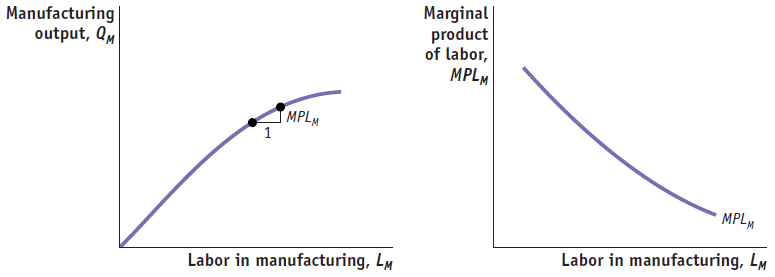
\includegraphics[width=0.95\textwidth]{tutorial2_specific_factors/production_function_mpl.png}
\end{center}


\begin{enumerate}
    \item Slope = $MPL_C$ (marginal product of labor)
    \item Diminishing returns: with K fixed, each additional worker has less capital to work with
    \item In Ricardo: constant MPL; here: diminishing MPL
\end{enumerate}

\end{frame}


\begin{frame}{Home - National Output Determination w/o trade: The Production Possibility Frontier (PPF)}

\textbf{Draw the Home PPF \& explain why the PPF in the specific factors model is curved (bowed out) rather than linear.}

\vspace{0.3cm}

\begin{enumerate}
    \item What does the slope of the PPF represent?
    \item What happens to the slope as we move along the PPF?
\end{enumerate}

\end{frame}

\begin{frame}{Home - National Output Determination w/o trade: PPF}
\vspace{-0.2cm}
\begin{center}
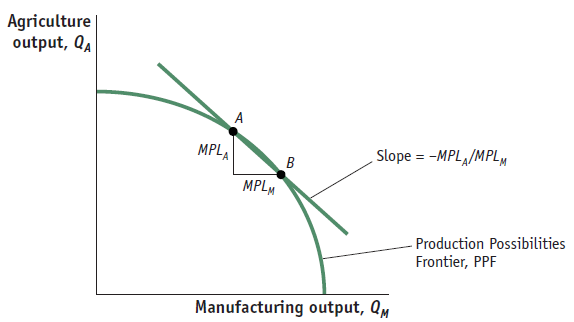
\includegraphics[width=0.9\textwidth]{tutorial2_specific_factors/home_national_output_ppf.png}
\end{center}
\vspace{-0.1cm}
\begin{enumerate}
    \item Slope of PPF = $-MPL_A / MPL_M$ = opportunity cost of manufacturing in terms of agriculture
    \item As we produce more $Q_M$: $MPL_M \downarrow$ and $MPL_A \uparrow$ $\Rightarrow$ slope becomes steeper (higher opportunity cost)
\end{enumerate}

\end{frame}

%========================
% Home Output with trade
%========================

\begin{frame}{Home - National Output Determination with Trade}

\textbf{When Home opens to trade, the relative price of manufacturing rises from $(P_M/P_A)$ to $(P_M/P_A)^W$. Show how this price change affects production.}

\vspace{0.3cm}

\begin{enumerate}
    \item Why does production shift from point A to point B?
    \item What happens to output in each sector ($Q_M$ and $Q_A$)?
\end{enumerate}

\end{frame}

\begin{frame}{Home - National Output Determination with Trade}
\vspace{-0.2cm}
\begin{center}
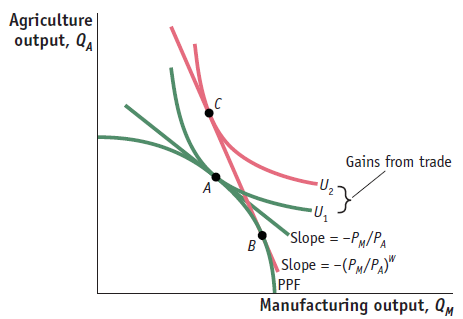
\includegraphics[width=0.8\textwidth]{tutorial2_specific_factors/home_national_output_ppf_with_trade}
\end{center}
\vspace{-0.1cm}
\begin{enumerate}
    \item $(P_M/P_A)^W > (P_M/P_A)$ makes manufacturing more profitable $\Rightarrow$ production shifts from A to B
    \item Manufacturing expands ($Q_M \uparrow$) for export; agriculture contracts ($Q_A \downarrow$) as Home imports from Foreign
\end{enumerate}

\end{frame}


%========================
% DETERMINATION OF WAGES - w/o & with trade
%========================
\begin{frame}{How do changes in output \& relative prices affect wages?}

\textbf{Using the labor allocation diagram, explain how wages are determined without trade and how they change when Home opens to trade.}

\vspace{0.3cm}

\begin{enumerate}
    \item What is the equilibrium condition for wage determination?
    \item When $P_C$ rises due to trade, what happens to the wage rate?
    \item Why does the wage rise by less than the price increase?
\end{enumerate}

\end{frame}


\begin{frame}{Wage Determination w/o trade}

\centering
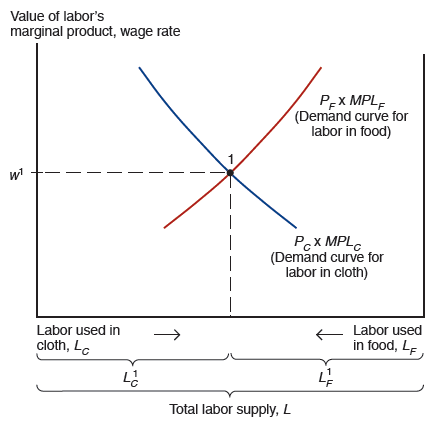
\includegraphics[height=0.75\textheight]{tutorial2_specific_factors/wage_determination1.png}

\vspace{-0.1cm}

\begin{enumerate}
    \item Equilibrium condition (labor mobility): $w = P_C \cdot MPL_C = P_F \cdot MPL_F$
\end{enumerate}
\end{frame}


\begin{frame}{Wage Determination with trade}

\begin{center}
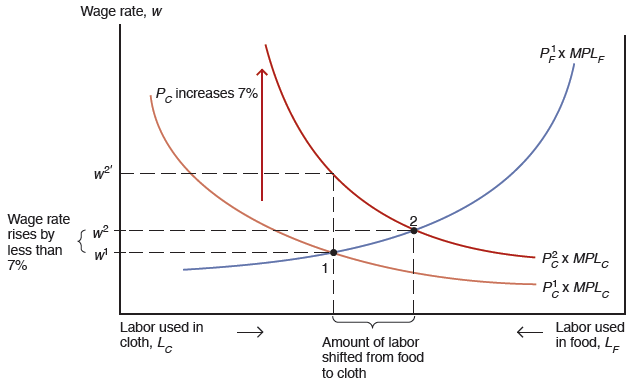
\includegraphics[width=0.75\textwidth]{tutorial2_specific_factors/wage_determination2.png}
\end{center}

\vspace{-0.1cm}

\small
\begin{enumerate}
    \setcounter{enumi}{1}
    \item $P_C$ rises, labor demand in cloth $\uparrow$, wages $\Rightarrow$, labor shifts to cloth
    \item Wage $\uparrow < P_C \uparrow$ as $P_C \uparrow$, but $MPL_C \downarrow$
    \item Gains/losses: Ambiguous as real wage $\uparrow$ in food, but $\downarrow$ in cloth
\end{enumerate}

\end{frame}





%========================
% Returns to Capital and Land - Setup
%========================
\begin{frame}{How does trade affect returns to capital and land?}

\textbf{Explain how we can calculate returns to specific factors (capital and land), and determine who wins and loses from trade.}

\vspace{0.3cm}

\begin{enumerate}
    \item What are the two ways of calculating returns to capital and land?
    
    
    \vspace{0.2cm}
    
    \item What general principle determines which specific factor owners benefit or lose from trade?
\end{enumerate}

\end{frame}


\begin{frame}{Returns to Capital and Land: Two Methods}

\textbf{How do we calculate returns to specific factors?}

\vspace{0.3cm}

\textbf{Method 1: Residual (Revenue $-$ Labor costs)}
\begin{align*}
\text{Profit in cloth} &= Q_C \times P_C - L_C \times w \\
\text{Rental on capital:} \quad R_K &= \frac{Q_C \times P_C - L_C \times w}{K}
\end{align*}

\vspace{0.3cm}

\textbf{Method 2: Marginal Product $\times$ Price}
$$R_K = P_C \times MPK$$

\vspace{0.3cm}

\textbf{Similarly for land:}
$$R_T = \frac{Q_F \times P_F - L_F \times w}{T} = P_F \times MPT$$

\end{frame}

%========================
% Returns to Capital - Effect of Trade
%========================

\begin{frame}{Effect of Trade on Returns to Capital}

\textbf{Capital is specific to cloth (the export sector).}

\vspace{0.3cm}

When $P_C$ rises due to trade opening:

\begin{itemize}
    \item Labor moves into cloth sector: $L_C \uparrow$
    
    \vspace{0.2cm}
    
    \item More labor per machine $\Rightarrow$ $MPK \uparrow$
    
    \vspace{0.2cm}
    
    \item $R_K = P_C \times MPK$ rises (both components increase!)
\end{itemize}

\vspace{0.3cm}

\textbf{Real returns to capital:}
\begin{itemize}
    \item $\frac{R_K}{P_C}$ \textbf{rises} (can buy more cloth)
    \item $\frac{R_K}{P_F}$ \textbf{rises even more} ($P_F$ unchanged)
\end{itemize}

\vspace{0.3cm}

$\Rightarrow$ \textcolor{capitalcolor}{\textbf{Capital owners are unambiguously BETTER OFF}}

\end{frame}

%========================
% Returns to Land - Effect of Trade
%========================

\begin{frame}{Effect of Trade on Returns to Land}

\textbf{Land is specific to food (the import-competing sector).}

\vspace{0.3cm}

When $P_C$ rises (and $P_F$ stays constant):

\begin{itemize}
    \item Labor leaves food sector: $L_F \downarrow$
    
    \vspace{0.2cm}
    
    \item Fewer workers per acre $\Rightarrow$ $MPT \downarrow$
    
    \vspace{0.2cm}
    
    \item $R_T = P_F \times MPT$ falls
\end{itemize}

\vspace{0.3cm}

\textbf{Real returns to land:}
\begin{itemize}
    \item $\frac{R_T}{P_F}$ \textbf{falls} (can buy less food)
    \item $\frac{R_T}{P_C}$ \textbf{falls even more} ($P_C$ increased)
\end{itemize}

\vspace{0.3cm}

$\Rightarrow$ \textcolor{landcolor}{\textbf{Landowners are unambiguously WORSE OFF}}

\end{frame}

%========================
% Summary: Winners and Losers
%========================

\begin{frame}{Summary: Winners and Losers from Trade}

\textbf{When relative price of cloth rises (cloth is the export good):}

\vspace{0.3cm}

\begin{center}
\begin{tabular}{lccc}
\toprule
\textbf{Factor} & \textbf{Real return} & \textbf{Real return} & \textbf{Overall} \\
& \textbf{in cloth} & \textbf{in food} & \\
\midrule
\textcolor{capitalcolor}{Capital (cloth)} & $\uparrow$ & $\uparrow$ & \textcolor{capitalcolor}{\textbf{Gains}} \\
\textcolor{landcolor}{Land (food)} & $\downarrow$ & $\downarrow$ & \textcolor{landcolor}{\textbf{Loses}} \\
\textcolor{laborcolor}{Labor (mobile)} & $\downarrow$ & $\uparrow$ & \textcolor{laborcolor}{\textbf{Ambiguous}} \\
\bottomrule
\end{tabular}
\end{center}

\vspace{0.5cm}

\textbf{General principle:}
\begin{itemize}
    \item Specific factor owners in \textbf{export} sector: \textbf{gains}
    \item Specific factor owners in \textbf{import-competing} sector: \textbf{loses}
    \item Mobile factor (labor): \textbf{ambiguous} \\ (consumption bundle, no unemployment)
\end{itemize}

\end{frame}

%========================
% Discussion Question
%========================

\begin{frame}{Question for Discussion: Trade Protection}

\textbf{Discussion tasks:}

\vspace{0.3cm}

\begin{enumerate}
    \item Think about examples of trade protection, trade opening, or lobbying from your countries of origin or residence.
    
    \vspace{0.3cm}
    
    \item Discuss your view on the pros and cons of trade opening in terms of specific factors.
    
    \vspace{0.3cm}
    
    \item Consider alternative policies:
    \begin{itemize}
        \item Compensation of losers via the welfare state
        \item Retraining programs
        \item Non-price factors (culture, professional/regional/gender identity)
    \end{itemize}
\end{enumerate}

\end{frame}

\subsubsection{Specific Factors \& Migration \& FDI}

%========================
% SECTION 2: MIGRATION & FDI
%========================

\begin{frame}

\vspace{2cm}

\centering
{\LARGE \textbf{Section 2}} \\[0.5cm]
{\Large The Specific Factors Model \& Migration \& FDI} \\[0.3cm]
{\large (Mobility of Labor \& Capital)}

\vfill

\end{frame}

%========================
% Transition: Factor Price Equalization
%========================

\begin{frame}{Factor Price Equalization (or Convergence)}

\textbf{Key insight:} Factors flow from where they are \textbf{abundant} (low marginal product) to where they are \textbf{scarce} (high marginal product).

\vspace{0.5cm}

\textbf{Three ways to achieve factor price convergence:}
\begin{itemize}
    \item \textbf{Trade} = Mobility of goods
    \item \textbf{Migration} = Mobility of labor
    \item \textbf{FDI} = Mobility of capital
\end{itemize}

\vspace{0.3cm}

\textit{These could be substitutes for achieving factor price equalization in the long run.}

\vspace{0.5cm}

\textbf{Today:} Short-run effects of migration and FDI through the specific factors lens.

\vspace{0.2cm}

\textit{No factor price equalization in the short run --- that's for next week (H-O model).}

\end{frame}

%========================
% Migration: Setup
%========================

\begin{frame}{Migration in the Specific Factors Model}

\textbf{Setup:} Labor migrates from Foreign (abundant) to Home (scarce).

\vspace{0.3cm}

\textbf{At Home (receiving country):}
\begin{itemize}
    \item Expansion of labor supply (at fixed K and T)
\end{itemize}

\textbf{At Foreign (sending country):}
\begin{itemize}
    \item Reduction of labor supply (at fixed K and T)
\end{itemize}

\vspace{0.3cm}

\textbf{Question:} What happens to wages and returns to specific factors?

\end{frame}

%========================
% Migration: Effect of inflow of migrants on home country
%========================

\begin{frame}{Migration: How does an increase in labor supply affect wages and output?}

\textbf{Suppose Home receives an inflow of immigrants ($\Delta L$). Using the labor allocation and PPF diagrams, analyze the effects.}

\vspace{0.3cm}

\begin{enumerate}
    \item What happens to the wage rate at Home?
    \item What happens to output in each sector ($Q_M$ and $Q_A$)?
    \item Who gains and who loses from immigration at Home?
\end{enumerate}

\end{frame}


\begin{frame}{Migration: Effect on Labor Allocation and Wages}
\begin{center}
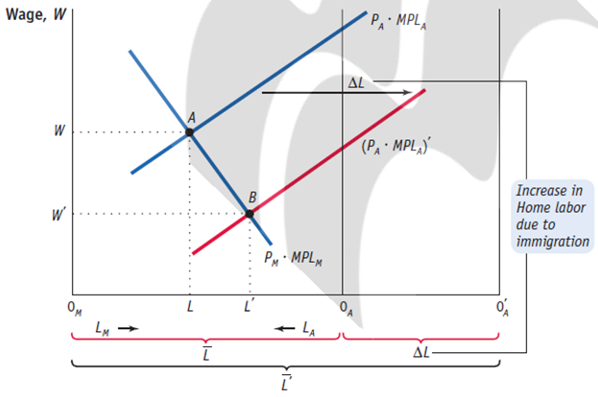
\includegraphics[width=0.8\textwidth]{tutorial2_specific_factors/migration1.png}
\end{center}
\begin{enumerate}
    \item Origin extends right as $\bar{L} \uparrow$; both sectors absorb workers
    \item $MPL_C \downarrow$ and $MPL_F \downarrow$ (more labor with fixed K and T)
    \item Wage falls: $W \rightarrow W'$
\end{enumerate}
\end{frame}

\begin{frame}{Migration: Effect on Output}

\begin{center}
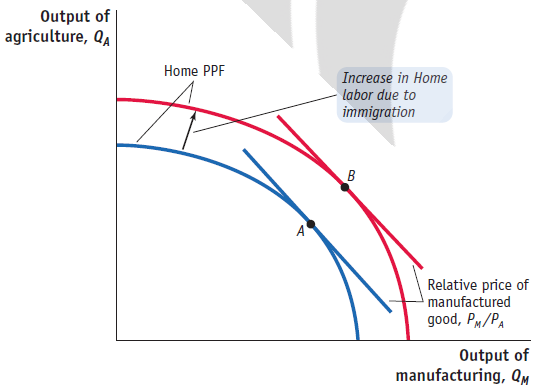
\includegraphics[width=0.7\textwidth]{tutorial2_specific_factors/migration2.png}
\end{center}

\begin{enumerate}
    \setcounter{enumi}{1}
    \item PPF expands; output rises in \textbf{both} sectors ($Q_M \uparrow$, $Q_A \uparrow$)
    \item Winners: Capital and land owners ($MPK \uparrow$, $MPT \uparrow$). Losers: Native workers (wages fall)
\end{enumerate}

\end{frame}



%========================
% FDI: Effect of inflow of FDI from home to FOR country
%========================

\begin{frame}{FDI: How does an increase in capital affect wages and output?}

\textbf{Suppose Home receives foreign direct investment (FDI), increasing the capital stock in manufacturing. Analyze the effects.}

\vspace{0.3cm}

\begin{enumerate}
    \item What happens to the wage rate at Home?
    \item What happens to output in each sector ($Q_M$ and $Q_A$)?
    \item Who gains and who loses from FDI at Home?
\end{enumerate}

\end{frame}

\begin{frame}{FDI: Effect on Labor Allocation, Wages, and Output}

\begin{center}
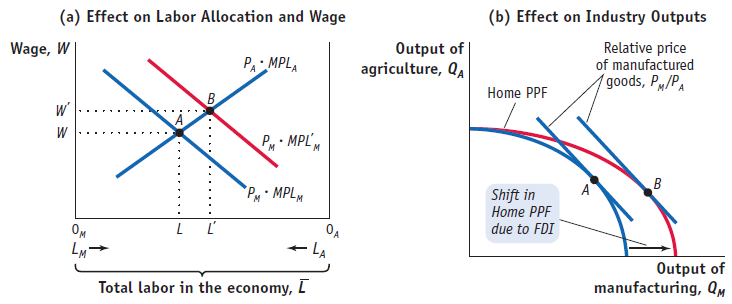
\includegraphics[width=0.95\textwidth]{tutorial2_specific_factors/fdi.png}
\end{center}

\begin{enumerate}
    \item Wage rises: $W \rightarrow W'$ (higher $MPL_M$ with more capital)
    \item PPF expands \textbf{biased toward manufacturing}; $Q_M \uparrow$, $Q_A \downarrow$
    \item Winners: Workers (wages rise). Losers: Landowners ($L_A \downarrow \Rightarrow MPT \downarrow$)
\end{enumerate}

\end{frame}

%========================
% Summary Comparison
%========================

\begin{frame}{Summary: Trade vs. Migration vs. FDI}
\begin{center}
\small
\begin{tabular}{lccc}
\toprule
& \textbf{Trade} & \textbf{Migration} & \textbf{FDI} \\
\midrule
What moves? & Goods & Labor & Capital \\
\midrule
Wages (Home) & Ambiguous & $\downarrow$ & $\uparrow$ \\
\midrule
$R_K$ (Home) & $\uparrow$* & $\uparrow$ & $\downarrow$ \\
\midrule
$R_T$ (Home) & $\downarrow$* & $\uparrow$ & $\downarrow$ \\
\midrule
PPF effect & PPF cst (CPF $\uparrow$) & $\uparrow$ (symmetric) & $\uparrow$ (biased) \\
\bottomrule
\end{tabular}
\end{center}
\footnotesize{*Assuming Home exports cloth (capital-intensive)} \\
\vspace{0.1cm}
\textbf{Key insight:} Trade, migration, and FDI can be \textbf{substitutes} for achieving factor price convergence, but have different distributional effects in the short run.
\end{frame}
%========================
% Summary
%========================

\begin{frame}{Summary: Key Takeaways}

\begin{enumerate}
    \item The specific factors model explains why trade creates \textbf{winners and losers} in the short run
    
    \vspace{0.2cm}
    
    \item \textbf{Specific factors} in export sectors gain; in import-competing sectors lose
    
    \vspace{0.2cm}
    
    \item \textbf{Mobile factors} (labor) have ambiguous welfare effects
    
    \vspace{0.2cm}
    
    \item \textbf{Migration} and \textbf{FDI} have different distributional effects:
    \begin{itemize}
        \item Immigration: workers lose, specific factors gain
        \item FDI: workers gain, specific factors lose
    \end{itemize}
    
    \vspace{0.2cm}
    
    \item Trade, migration, and FDI can be \textbf{substitutes} for factor price convergence
\end{enumerate}

\vspace{0.3cm}

\textit{Next week: Heckscher-Ohlin model --- the long-run view where all factors are mobile.}

\end{frame}


\fi


\ifnum\showanswers=0

\subsection{Specific Factors w/o Answers}

\subsubsection{Introduction}
%========================
% Slide 1: Title Slide
%========================

\begin{frame}

\vspace{1.5cm}

\centering
{\Large \textbf{Tutorial 2: Specific Factors and Income Distribution}} \\[0.5cm]
{\large Short-Run Effects of Trade, Migration, and FDI} \\[1.0cm]

{\small 7QQMM209: International Economics} \\[0.3cm]
{\small King's College London}

\vfill

\end{frame}

%========================
% Slide 2: Agenda
%========================

\begin{frame}{Agenda}

\begin{enumerate}
    \item \textbf{Ricardian Trade vs. Specific Factors Model} \\~\\
    
    \item \textbf{Specific Factors Model: Trade Opening}
    \begin{itemize}
        \item Determination of Output
        \item Determination of Wages
        \item Distribution of Gains and Losses
    \end{itemize}
    
    \vspace{0.3cm}
    
    \item \textbf{Specific Factors Model: Migration} \\~\\
    
    \item \textbf{Specific Factors Model: FDI}
\end{enumerate}

\end{frame}

%========================
% Slide 3: References
%========================

\begin{frame}{References: Textbook Chapters}

\textbf{Primary readings:}
\begin{itemize}
    \item \textbf{KOM:} Chapter 4 --- Specific Factors and Income Distribution \\~\\
    \item \textbf{Feenstra \& Taylor:} Chapter 3 --- Gains and Losses from Trade in the Specific Factors Model \\~\\
    \item \textbf{Feenstra \& Taylor:} Chapter 5 --- Movement of Labor and Capital between Countries
\end{itemize}
\end{frame}

%========================
% Slide 4: Concepts Overview
%========================

\begin{frame}{Key Concepts for This Tutorial}

\begin{itemize}
    \item \textbf{Specific (fixed, stuck) vs. general-purpose factors}
    \begin{itemize}
        \item ``Sector-switching costs''
    \end{itemize}
    
    \vspace{0.3cm}
    
    \item \textbf{Marginal product of labor, capital, and land}
    
    \vspace{0.3cm}
    
    \item \textbf{Production function} (with diminishing returns)
    
    \vspace{0.3cm}
    
    \item \textbf{Production Possibility Frontier} (curved, not linear)
    
    \vspace{0.3cm}
    
    \item \textbf{Two ways of calculating returns to capital and land:}
    \begin{enumerate}
        \item Revenue $-$ Labor costs $=$ Profit $\Rightarrow R_K = \frac{\text{Profit}}{K}$
        \item Marginal product $\times$ Price: $R_K = P \times MPK$
    \end{enumerate}
\end{itemize}

\end{frame}

%========================
% Slide : Trade models overview
%========================
\begin{frame}{Where Does the Specific Factors Model Fit?}

\textbf{Evolution of Trade Theory:}

\vspace{0.3cm}

\begin{tabular}{lp{7cm}}
\textbf{1817} & \textbf{Ricardo:} Comparative advantage, labor only \\[0.2cm]
\textbf{1930s} & \textbf{Heckscher-Ohlin:} Multiple mobile factors (long-run) \\[0.2cm]
\textbf{1971} & \textbf{Samuelson \& Jones:} \textit{Specific Factors Model} --- some factors immobile (short-run)
\end{tabular}

\vspace{0.5cm}

\textbf{Key insight:} The distinction between ``short-run'' and ``long-run'' is about \textbf{factor mobility}, not calendar time.

\end{frame}

%========================
% Slide 5: Key Difference from Ricardo/ Transition from Ricardo
%========================
\begin{frame}{Transition Question: How Does the Specific Factors Model Differ from the Ricardian Model?}

\begin{columns}[T]
\begin{column}{0.48\textwidth}
\textbf{Ricardian Model}
\begin{itemize}
    \item One factor: Labor
    \item Labor fully mobile
    \item Constant MPL
    \item Linear PPF
    \item Everyone benefits from trade
\end{itemize}
\end{column}

\begin{column}{0.48\textwidth}
\textbf{Specific Factors Model}
\begin{itemize}
    \item Three factors: L, K, T
    \item K and T specific (immobile)
    \item \textbf{Diminishing} MPL
    \item \textbf{Curved} PPF
    \item Winners \textbf{and} losers
\end{itemize}
\end{column}
\end{columns}

\vspace{0.5cm}

\textbf{Key implication:} Trade can differentially affect income, even though it is beneficial for a country as a whole.

\end{frame}

%========================
% Slide: Question - Examples
%========================

\begin{frame}{Question: Examples of Specific vs. General-Purpose Factors}

\textbf{Task:} Make a list of examples for specific and general-purpose factors of production.

\vspace{0.3cm}

Find 1--2 examples for \textbf{each} of the following:

\vspace{0.3cm}

\begin{center}
\begin{tabular}{l|c|c}
\toprule
\textbf{Factor Type} & \textbf{Specific} & \textbf{General-Purpose} \\
\midrule
Labor (skills) & ? & ? \\
\midrule
Capital & ? & ? \\
\midrule
Land / Raw materials & ? & ? \\
\bottomrule
\end{tabular}
\end{center}

\vspace{0.5cm}

\textit{Hint:} Think about how easily each factor can be redeployed to another sector or activity.

\end{frame}


\subsubsection{Specific Factors \& Trade}
%========================
% SECTION slide
%========================
\begin{frame}

\vspace{2cm}

\centering
{\LARGE \textbf{Section 1}} \\[0.5cm]
{\Large The Specific Factors Model \& Trade} \\[0.3cm]
{\large (Mobility of Goods)}

\vfill

\end{frame}

%========================
% Model Set-Up
%========================
\begin{frame}{Model Set-Up: Key Ingredients}

\textbf{Two Sectors:}
\begin{itemize}
    \item Food / Agriculture (F)
    \item Cloth / Manufacturing (C)
\end{itemize}

\vspace{0.2cm}

\textbf{Three Factors of Production:}
\begin{itemize}
    \item \textcolor{laborcolor}{\textbf{Labor (L):}} Mobile, used in both sectors
    \item \textcolor{landcolor}{\textbf{Land (T):}} Specific to food/agriculture only
    \item \textcolor{capitalcolor}{\textbf{Capital (K):}} Specific to cloth/manufacturing only
\end{itemize}

\vspace{0.2cm}

\textbf{Production Functions:}
\begin{align*}
Q_F &= Q_F(T, L_F) \quad \text{(Food)} \\
Q_C &= Q_C(K, L_C) \quad \text{(Cloth)}
\end{align*}

\textbf{Labor Supply Constraint:} $L = L_C + L_F$

\vspace{0.2cm}

\textbf{Price Differential (Home has CA in cloth):}
$$\left(\frac{P_C}{P_F}\right)^{\text{Home}} < \left(\frac{P_C}{P_F}\right)^{W} < \left(\frac{P_C}{P_F}\right)^{\text{Foreign}}$$

\end{frame}

%========================
% Home Output w/o trade - QUESTION ONLY
%========================
\begin{frame}{Home - Sectoral Output Determination w/o trade: The Production Function}

\textbf{Draw the production function for cloth, showing the relationship between labor input ($L_C$) and output ($Q_C$), holding capital fixed. Also draw the derivative.}

\vspace{0.2cm}

\textit{Axes: x-axis = Labor input in cloth ($L_C$); y-axis = Output of cloth ($Q_C$) for the production function, and $MPL_C$ for the derivative.}

\vspace{0.3cm}

\begin{enumerate}
    \item What does the slope of this curve represent?
    \item Why does the curve get flatter as $L_C$ increases?
    \item How does this differ from the Ricardian model?
\end{enumerate}

\end{frame}


\begin{frame}{Home - National Output Determination w/o trade: The Production Possibility Frontier (PPF)}

\textbf{Draw the Home PPF \& explain why the PPF in the specific factors model is curved (bowed out) rather than linear.}

\vspace{0.2cm}

\textit{Axes: x-axis = Output of cloth ($Q_C$); y-axis = Output of food ($Q_F$).}

\vspace{0.3cm}

\begin{enumerate}
    \item What does the slope of the PPF represent?
    \item What happens to the slope as we move along the PPF?
\end{enumerate}

\end{frame}

%========================
% Home Output with trade - QUESTION ONLY
%========================

\begin{frame}{Home - National Output Determination with Trade}

\textbf{When Home opens to trade, the relative price of manufacturing rises from $(P_M/P_A)$ to $(P_M/P_A)^W$. Show how this price change affects production.}

\vspace{0.2cm}

\textit{Axes: x-axis = Output of manufacturing ($Q_M$); y-axis = Output of agriculture ($Q_A$).}

\vspace{0.3cm}

\begin{enumerate}
    \item Why does production shift from point A to point B?
    \item What happens to output in each sector ($Q_M$ and $Q_A$)?
\end{enumerate}

\end{frame}


%========================
% DETERMINATION OF WAGES - QUESTION ONLY
%========================
\begin{frame}{How do changes in output \& relative prices affect wages?}

\textbf{Using the labor allocation diagram, explain how wages are determined without trade and how they change when Home opens to trade.}

\vspace{0.2cm}

\textit{Axes: x-axis = Labor in cloth ($L_C$, increasing left to right) and Labor in food ($L_F$, increasing right to left); y-axis = Wage ($w$) or value of marginal product ($P \times MPL$).}

\vspace{0.3cm}

\begin{enumerate}
    \item What is the equilibrium condition for wage determination?
    \item When $P_C$ rises due to trade, what happens to the wage rate?
    \item Why does the wage rise by less than the price increase?
\end{enumerate}

\end{frame}


%========================
% Returns to Capital and Land - QUESTION ONLY
%========================
\begin{frame}{How does trade affect returns to capital and land?}

\textbf{Explain how we can calculate returns to specific factors (capital and land), and determine who wins and loses from trade.}

\vspace{0.3cm}

\begin{enumerate}
    \item What are the two ways of calculating returns to capital and land?
    
    
    \vspace{0.2cm}
    
    \item What general principle determines which specific factor owners benefit or lose from trade?
\end{enumerate}

\end{frame}


%========================
% Discussion Question
%========================

\begin{frame}{Question for Discussion: Trade Protection}

\textbf{Discussion tasks:}

\vspace{0.3cm}

\begin{enumerate}
    \item Think about examples of trade protection, trade opening, or lobbying from your countries of origin or residence.
    
    \vspace{0.3cm}
    
    \item Discuss your view on the pros and cons of trade opening in terms of specific factors.
    
    \vspace{0.3cm}
    
    \item Consider alternative policies:
    \begin{itemize}
        \item Compensation of losers via the welfare state
        \item Retraining programs
        \item Non-price factors (culture, professional/regional/gender identity)
    \end{itemize}
\end{enumerate}

\end{frame}

\subsubsection{Specific Factors \& Migration \& FDI}

%========================
% SECTION 2: MIGRATION & FDI
%========================

\begin{frame}

\vspace{2cm}

\centering
{\LARGE \textbf{Section 2}} \\[0.5cm]
{\Large The Specific Factors Model \& Migration \& FDI} \\[0.3cm]
{\large (Mobility of Labor \& Capital)}

\vfill

\end{frame}

%========================
% Transition: Factor Price Equalization
%========================

\begin{frame}{Factor Price Equalization (or Convergence)}

\textbf{Key insight:} Factors flow from where they are \textbf{abundant} (low marginal product) to where they are \textbf{scarce} (high marginal product).

\vspace{0.5cm}

\textbf{Three ways to achieve factor price convergence:}
\begin{itemize}
    \item \textbf{Trade} = Mobility of goods
    \item \textbf{Migration} = Mobility of labor
    \item \textbf{FDI} = Mobility of capital
\end{itemize}

\vspace{0.3cm}

\textit{These could be substitutes for achieving factor price equalization in the long run.}

\vspace{0.5cm}

\textbf{Today:} Short-run effects of migration and FDI through the specific factors lens.

\vspace{0.2cm}

\textit{No factor price equalization in the short run --- that's for next week (H-O model).}

\end{frame}

%========================
% Migration: Setup
%========================

\begin{frame}{Migration in the Specific Factors Model}

\textbf{Setup:} Labor migrates from Foreign (abundant) to Home (scarce).

\vspace{0.3cm}

\textbf{At Home (receiving country):}
\begin{itemize}
    \item Expansion of labor supply (at fixed K and T)
\end{itemize}

\textbf{At Foreign (sending country):}
\begin{itemize}
    \item Reduction of labor supply (at fixed K and T)
\end{itemize}

\vspace{0.3cm}

\textbf{Question:} What happens to wages and returns to specific factors?

\end{frame}

%========================
% Migration: Effect of inflow of migrants on home country - QUESTION ONLY
%========================

\begin{frame}{Migration: How does an increase in labor supply affect wages and output?}

\textbf{Suppose Home receives an inflow of immigrants ($\Delta L$). Using the labor allocation and PPF diagrams, analyze the effects.}

\vspace{0.2cm}

\textit{Labor allocation diagram axes: x-axis = Labor ($L$, with $L_M$ increasing left to right, $L_A$ increasing right to left); y-axis = Wage ($w$).}

\vspace{0.1cm}

\textit{PPF diagram axes: x-axis = Output of manufacturing ($Q_M$); y-axis = Output of agriculture ($Q_A$).}

\vspace{0.3cm}

\begin{enumerate}
    \item What happens to the wage rate at Home?
    \item What happens to output in each sector ($Q_M$ and $Q_A$)?
    \item Who gains and who loses from immigration at Home?
\end{enumerate}

\end{frame}



%========================
% FDI: Effect of inflow of FDI from home to FOR country - QUESTION ONLY
%========================

\begin{frame}{FDI: How does an increase in capital affect wages and output?}

\textbf{Suppose Home receives foreign direct investment (FDI), increasing the capital stock in manufacturing. Analyze the effects.}

\vspace{0.2cm}

\textit{Labor allocation diagram axes: x-axis = Labor ($L$, with $L_M$ increasing left to right, $L_A$ increasing right to left); y-axis = Wage ($w$).}

\vspace{0.1cm}

\textit{PPF diagram axes: x-axis = Output of manufacturing ($Q_M$); y-axis = Output of agriculture ($Q_A$).}

\vspace{0.3cm}

\begin{enumerate}
    \item What happens to the wage rate at Home?
    \item What happens to output in each sector ($Q_M$ and $Q_A$)?
    \item Who gains and who loses from FDI at Home?
\end{enumerate}

\end{frame}


%========================
% Summary
%========================

\begin{frame}{Summary: Key Takeaways}

\begin{enumerate}
    \item The specific factors model explains why trade creates \textbf{winners and losers} in the short run
    
    \vspace{0.2cm}
    
    \item \textbf{Specific factors} in export sectors gain; in import-competing sectors lose
    
    \vspace{0.2cm}
    
    \item \textbf{Mobile factors} (labor) have ambiguous welfare effects
    
    \vspace{0.2cm}
    
    \item \textbf{Migration} and \textbf{FDI} have different distributional effects:
    \begin{itemize}
        \item Immigration: workers lose, specific factors gain
        \item FDI: workers gain, specific factors lose
    \end{itemize}
    
    \vspace{0.2cm}
    
    \item Trade, migration, and FDI can be \textbf{substitutes} for factor price convergence
\end{enumerate}

\vspace{0.3cm}

\textit{Next week: Heckscher-Ohlin model --- the long-run view where all factors are mobile.}

\end{frame}

\fi


% Tutorial 3: Heckscher-Ohlin Model
% Structure mirrors Tutorial 2 (Specific Factors with Answers)
% Add this after the Specific Factors subsection in main_international_economics__2_.tex
\ifnum\showanswers=0
\subsection{Heckscher-Ohlin with Answers}

\subsubsection{Introduction}
%========================
% Slide 1: Title Slide
%========================

\begin{frame}

\vspace{1.5cm}

\centering
{\Large \textbf{Tutorial 3: Factor Endowments and Income Distribution}} \\[0.5cm]
{\large The Heckscher-Ohlin Model (Long-Run)} \\[1.0cm]

{\small 7QQMM209: International Economics} \\[0.3cm]
{\small King's College London}

\vfill

\end{frame}

%========================
% Slide 2: Agenda
%========================

\begin{frame}{Agenda}

\begin{enumerate}
    \item \textbf{From Specific Factors to Heckscher-Ohlin}
    \begin{itemize}
        \item Short-run vs.\ long-run: What changes?
    \end{itemize}
    
    \vspace{0.3cm}
    
    \item \textbf{HO Model: Output Determination}
    \begin{itemize}
        \item PPF shape and factor abundance
        \item Production with and without trade
    \end{itemize}
    
    \vspace{0.3cm}
    
    \item \textbf{HO Model: Factor Price Determination}
    \begin{itemize}
        \item Wage and rental with and without trade
        \item Stolper-Samuelson theorem
    \end{itemize}
    
    \vspace{0.3cm}
    
    \item \textbf{Gains and Losses from Trade}
    \begin{itemize}
        \item Who wins? Who loses? (Income distribution)
    \end{itemize}
\end{enumerate}

\end{frame}

%========================
% Slide 3: References
%========================

\begin{frame}{References: Textbook Chapters}

\textbf{Primary readings:}
\begin{itemize}
    \item \textbf{KOM:} Chapter 5 --- Resources and Trade: The Heckscher-Ohlin Model \\~\\
    \item \textbf{Feenstra \& Taylor:} Chapter 4, Sections 1 \& 3 --- Trade and Resources: The Heckscher-Ohlin Model (pp.\ 88--94, 109--114)
\end{itemize}

\vspace{0.5cm}

\textbf{Key figures to study:}
\begin{itemize}
    \item Feenstra Figures 4-1, 4-2, 4-3, 4-10, 4-11, 4-12
    \item KOM Figures 5-5, 5-8, 5-11
\end{itemize}

\end{frame}

%========================
% Slide 4: Key Concepts
%========================

\begin{frame}{Key Concepts for This Tutorial}

\begin{itemize}
    \item \textbf{Factor abundance} vs.\ \textbf{factor intensity}
    
    \vspace{0.3cm}
    
    \item \textbf{Factor intensity} and \textbf{input choice} ($L/K$ ratio)
    
    \vspace{0.3cm}
    
    \item \textbf{Biased PPF} (skewed toward abundant-factor-intensive good)
    
    \vspace{0.3cm}
    
    \item \textbf{Production vs.\ Consumption Possibility Frontier}
    
    \vspace{0.3cm}
    
    \item \textbf{Stolper-Samuelson theorem:} magnification effect of price changes on factor returns
    
    \vspace{0.3cm}
    
    \item \textbf{Abundant factor gains, scarce factor loses} from trade
\end{itemize}

\end{frame}


%========================
% Slide 5: Transition from Specific Factors to HO
%========================

%========================
% Slide 5a: Transition Question
%========================
\begin{frame}{What are the key differences between Ricardo, Specific Factors, and HO?}

\vspace{0.3cm}

Think about:
\begin{enumerate}
    \item How many factors of production? Which are mobile?
    \item What determines the shape of the PPF?
    \item Who gains and who loses from trade?
    \item Are these effects temporary or permanent?
\end{enumerate}

\end{frame}

%========================
% Slide 5b: Transition Answer
%========================
\begin{frame}{Transition: From Specific Factors to Heckscher-Ohlin}

\begin{columns}[T]
\begin{column}{0.48\textwidth}
\textbf{Specific Factors (Short-Run)}
\begin{itemize}
    \item 3 factors: L, K, T
    \item K and T \textbf{immobile} (stuck), L \textbf{mobile}
    \item Specific factors: clear win/lose
    \item Mobile factor: ambiguous
    \item Gains/losses may be \textbf{temporary}
\end{itemize}
\end{column}

\begin{column}{0.48\textwidth}
\textbf{Heckscher-Ohlin (Long-Run)}
\begin{itemize}
    \item 2 factors: L, K
    \item \textbf{Both fully mobile} across sectors
    \item Producers \textbf{choose} L/K ratio
    \item Clear winners and losers
    \item Gains/losses are \textbf{permanent}
\end{itemize}
\end{column}
\end{columns}

\vspace{0.5cm}

\textbf{Key difference:} In the long run, all factors can move between sectors. Income distribution is determined by \textbf{factor type} (labor vs.\ capital), not by sector of employment.

\end{frame}


\subsubsection{HO Model \& Trade}
%========================
% SECTION slide
%========================
\begin{frame}

\vspace{2cm}

\centering
{\LARGE \textbf{Section 1}} \\[0.5cm]
{\Large The Heckscher-Ohlin Model \& Trade} \\[0.3cm]
{\large (Mobility of Goods)}

\vfill

\end{frame}

%========================
% Model Set-Up
%========================
\begin{frame}{Model Set-Up: Key Ingredients}

\textbf{Two Countries:} Home, Foreign

\textbf{Two Goods:} Computers (C), Shoes (S)

\textbf{Two Factors:} Labor (L), Capital (K) - both mobile across sectors

\vspace{0.3cm}

\textbf{Key Assumptions:}
\begin{enumerate}
    \item \textbf{Same technology} in both countries
    \item \textbf{Factor intensity:} Computers are capital-intensive ($K_C/L_C > K_S/L_S$); Shoes are labor-intensive ($L_S/K_S > L_C/K_C$)
    \item \textbf{Factor abundance:} Home is capital-abundant ($\bar{K}/\bar{L} > \bar{K}^*/\bar{L}^*$); Foreign is labor-abundant
    \item Same preferences (identical, homothetic)
    \item Free trade, no transport costs
    \item Both countries produce both goods
\end{enumerate}

\vspace{0.3cm}

\textbf{Price Differential (Home has CA in computers):}
$$\left(\frac{P_C}{P_S}\right)^{\text{Home}} < \left(\frac{P_C}{P_S}\right)^{W} < \left(\frac{P_C}{P_S}\right)^{\text{Foreign}}$$

\end{frame}

%========================
% Q1: Factor Intensity & Input Choice - QUESTION
%========================
\begin{frame}{How do producers choose between labor and capital?}

\textbf{Using a diagram with the wage-rental ratio ($W/R$) on the vertical axis and the labor-capital ratio ($L/K$) on the horizontal axis, show the input choice for computers and shoes.}

\vspace{0.2cm}

\textit{Axes: x-axis = Labor-capital ratio ($L/K$); y-axis = Wage-rental ratio ($W/R$).}

\vspace{0.3cm}

\begin{enumerate}
    \item Why do the relative factor demand curves slope downward?
    \item Which curve lies further to the right, and why?
    \item What happens to input choices when $W/R$ changes?
\end{enumerate}

\end{frame}

%========================
% Q1: Factor Intensity & Input Choice - ANSWER
%========================
\begin{frame}{Factor Intensity and Input Choice}

% Placeholder for figure: Feenstra Figure 4-1 / KOM Figure 5-5
% Two downward-sloping curves: L_S/K_S (shoes, further right) and L_C/K_C (computers, further left)
% x-axis: L/K, y-axis: W/R

\begin{center}
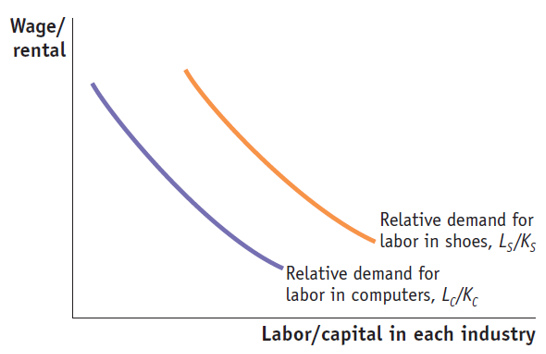
\includegraphics[height=0.5\textheight]{tutorial3_heckscher_ohlin/feenstra_4_1_wage_rcap_labor_capital_ratio.png}
\end{center}

\begin{enumerate}
    \item When $W/R$ rises (labor becomes relatively expensive), firms in \textbf{both} sectors substitute toward capital $\Rightarrow$ $L/K$ falls
    \item Shoes curve ($L_S/K_S$) lies to the right: shoes always use more labor per unit of capital than computers, at any $W/R$
    \item A rise in $W/R$ reduces $L/K$ in both sectors, but the \textbf{ranking} is preserved (no factor intensity reversal)
\end{enumerate}

\end{frame}


%========================
% Q2: PPF Shape & No-Trade Equilibrium - QUESTION (combined)
%========================
\begin{frame}{How does factor abundance shape the PPF and determine no-trade prices?}

\textbf{Draw the PPFs for Home (capital-abundant) and Foreign (labor-abundant), with indifference curves showing the autarky equilibrium.}

\vspace{0.2cm}

\textit{Axes: x-axis = Output of computers ($Q_C$); y-axis = Output of shoes ($Q_S$).}

\vspace{0.3cm}

\begin{enumerate}
    \item In which direction is each country's PPF skewed, and why?
    \item Where is the no-trade equilibrium? Which country has a lower $P_C/P_S$?
    \item What does this imply for the pattern of trade?
\end{enumerate}

\end{frame}

%========================
% Q2: PPF Shape & No-Trade Equilibrium - ANSWER (combined)
%========================
\begin{frame}{PPF Shape and No-Trade Prices Reflect Factor Abundance}

\begin{center}
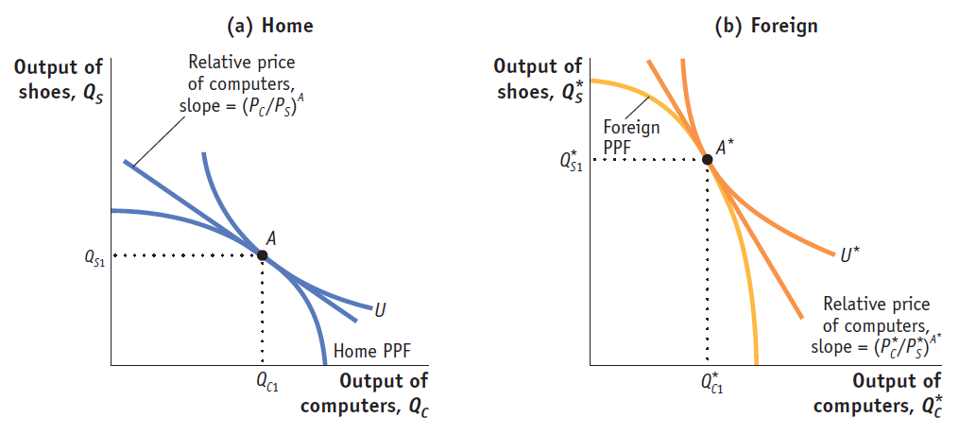
\includegraphics[width=0.9\textwidth]{tutorial3_heckscher_ohlin/feenstra_4_2_ppf_autarky.png}
\end{center}

\begin{enumerate}
    \item Home PPF skewed toward \textbf{computers} (capital-abundant, computers capital-intensive); Foreign PPF skewed toward \textbf{shoes} (labor-abundant, shoes labor-intensive)
    \item Autarky equilibrium where indifference curve is tangent to PPF. Home has \textbf{lower} $P_C/P_S$ (flat price line); Foreign has \textbf{higher} $P_C/P_S$ (steep price line)
    \item Home exports computers, imports shoes; Foreign does the reverse
\end{enumerate}

\vspace{0.2cm}

$\Rightarrow$ \textbf{HO Theorem:} A country exports the good that uses its \textbf{abundant factor} intensively.

\end{frame}

%========================
% Q4: Production & Consumption with Trade - QUESTION
%========================
\begin{frame}{How does trade change production and consumption possibilities?}

\textbf{When Home opens to trade, the world relative price of computers $(P_C/P_S)^W$ is higher than Home's autarky price. Show how production and consumption change.}

\vspace{0.2cm}

\textit{Axes: x-axis = Output of computers ($Q_C$); y-axis = Output of shoes ($Q_S$).}

\vspace{0.3cm}

\begin{enumerate}
    \item How does the production point move along the PPF?
    \item How can the consumption point lie \textbf{outside} the PPF?
    \item Draw the ``trade triangle'' and identify exports and imports.
\end{enumerate}

\end{frame}

%========================
% Q4: Production & Consumption with Trade - ANSWER
%========================
\begin{frame}{Trade Expands Consumption Beyond the PPF}

% Placeholder: Feenstra Figure 4-3 (Home with free trade)
% Production at B (more computers, fewer shoes), consumption at C (on higher indifference curve)
% World price line through B, tangent to higher U

\begin{center}
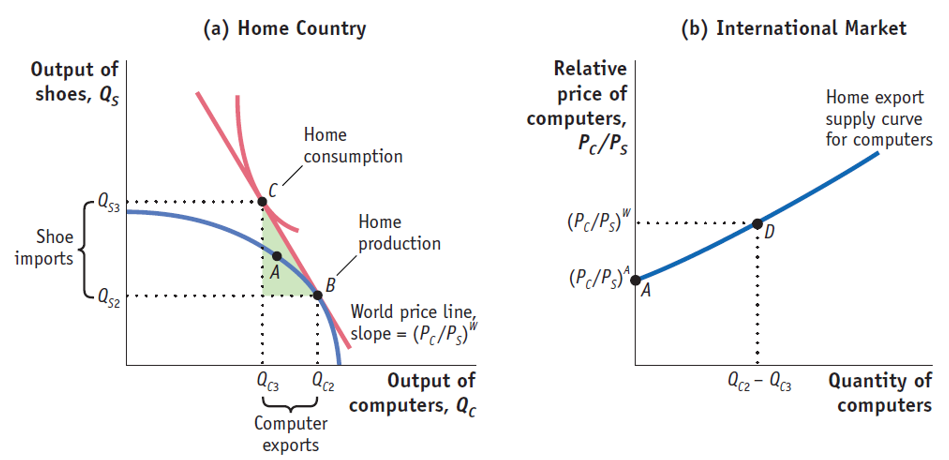
\includegraphics[width=0.9\textwidth]{tutorial3_heckscher_ohlin/feenstra_4_3_ppf_trade.png}
\end{center}

\begin{enumerate}
    \item Production shifts from A to B: more computers, fewer shoes ($(P_C/P_S)^W$ makes computers more profitable)
    \item With trade, Home can \textbf{consume at point C} on the world price line through B --- this lies on a \textbf{higher indifference curve} than the PPF allows in autarky
    \item Trade triangle: Home exports computers ($Q_{C2} - Q_{C3}$), imports shoes ($Q_{S3} - Q_{S2}$)
\end{enumerate}

\vspace{0.2cm}

\textbf{Key:} The consumption possibility frontier (world price line) lies \textbf{outside} the PPF $\Rightarrow$ gains from trade for the country as a whole.

\end{frame}


%========================
% Q5a: Effect on Factor Prices - QUESTION (Figure)
%========================
\begin{frame}{Q5a: How does trade affect $W/R$? (Diagram)}
\textbf{Using the economy-wide relative demand for labor diagram, explain how trade changes $W/R$ at Home (capital-abundant).}
\vspace{0.2cm}
\textit{Axes: x-axis = $L/K$; \; y-axis = $W/R$.}
\vspace{0.3cm}
\begin{enumerate}
    \item How does $(P_C/P_S) \uparrow$ shift the economy-wide RD curve?
    \item What happens to $W/R$?
    \item What happens to $L/K$ ratios in \textbf{both} sectors?
\end{enumerate}
\end{frame}

%========================
% Q5a: Effect on Factor Prices - ANSWER (Figure)
%========================
\begin{frame}{Q5a Answer: Economy-Wide Relative Demand Diagram}
% Placeholder: Feenstra Figure 4-12
\begin{center}
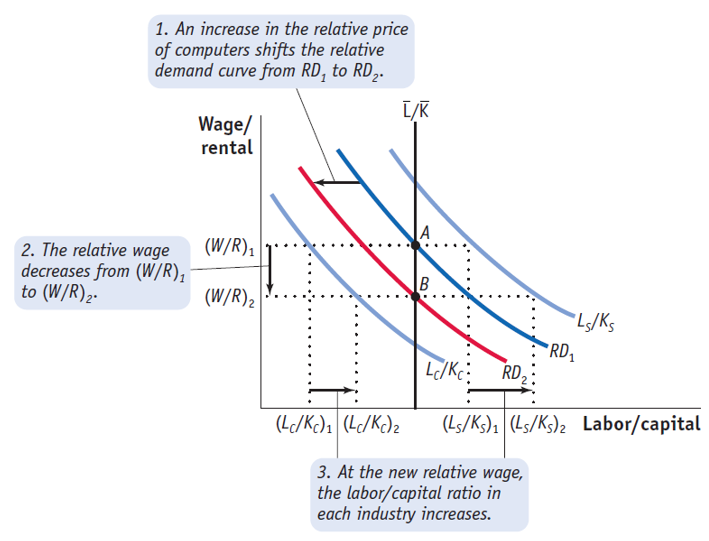
\includegraphics[width=0.6\textwidth]{tutorial3_heckscher_ohlin/feenstra_4_11_factor_prices_trade.png}
\end{center}
\small
\begin{enumerate}
    \item $(P_C/P_S) \uparrow$ $\Rightarrow$ RD shifts toward capital-intensive computers: $RD_1 \to RD_2$
    \item Equilibrium moves $A \to B$: $W/R$ \textbf{falls}
    \item Lower $W/R$ $\Rightarrow$ both sectors substitute toward cheaper labor $\Rightarrow$ $L_C/K_C \uparrow$ and $L_S/K_S \uparrow$
\end{enumerate}
\end{frame}

%========================
% Q5b: Stolper-Samuelson - QUESTION (Equation / P x MP logic)
%========================
\begin{frame}{Q5b: Who gains, who loses? (Stolper-Samuelson)}
\textbf{Using the competitive pricing conditions $W = P \cdot MPL$ and $R = P \cdot MPK$, explain why the factor used intensively in the rising-price good gains more than proportionally.}
\vspace{0.3cm}
\begin{enumerate}
    \item What happens to $MPK$ and $MPL$ when $L/K$ rises in both sectors?
    \item How do changes in $P_C$, $MPK$, and $MPL$ affect the \textbf{real} rental and wage?
    \item State the Stolper-Samuelson theorem.
\end{enumerate}
\end{frame}

%========================
% Q5b: Stolper-Samuelson - ANSWER (Equation / P x MP logic)
%========================
\begin{frame}{Q5b Answer: The $P \times MP$ Logic (Stolper-Samuelson)}
\textbf{Competitive pricing (recall Tutorial 2):}
$$W = P_C \cdot MPL_C = P_S \cdot MPL_S \qquad R = P_C \cdot MPK_C = P_S \cdot MPK_S$$

\small
\textbf{When $(P_C/P_S) \uparrow$ and $L/K \uparrow$ in both sectors:}

\vspace{0.15cm}

\begin{itemize}
    \item \textbf{Capital} (intensive in computers): $MPK \uparrow$ (more workers per machine)
    \begin{itemize}
        \item $R = P_C \cdot MPK_C$: both $P_C \uparrow$ and $MPK_C \uparrow$ $\Rightarrow$ $R \uparrow\uparrow$ \; (\textbf{magnified} gain)
        \item $R/P_C \uparrow$ and $R/P_S \uparrow$ $\Rightarrow$ \textcolor{myblue}{\textbf{capital owners unambiguously better off}}
    \end{itemize}

    \vspace{0.15cm}

    \item \textbf{Labor} (intensive in shoes): $MPL \downarrow$ (diminishing returns)
    \begin{itemize}
        \item $W = P_S \cdot MPL_S$: $P_S$ unchanged, $MPL_S \downarrow$ $\Rightarrow$ $W \downarrow$
        \item $W/P_C \downarrow$ and $W/P_S \downarrow$ $\Rightarrow$ \textcolor{foreigncolor}{\textbf{workers unambiguously worse off}}
    \end{itemize}
\end{itemize}

\vspace{0.2cm}

\normalsize
\textbf{Stolper-Samuelson:} $\Delta W/W < 0 < \Delta P_C/P_C < \Delta R/R$

\vspace{0.1cm}

\small
\textit{Contrast with Tutorial 2:} In the specific factors model, labor's real wage was \textit{ambiguous}. In HO, because all factors are mobile, the result is \textbf{unambiguous} --- the magnification effect.
\end{frame}
%========================
% Q7: Summary - Winners and Losers
%========================
\begin{frame}{Summary: Winners and Losers from Trade (Long-Run)}

\textbf{When Home (capital-abundant) opens to trade:}

\vspace{0.3cm}

\begin{center}
\begin{tabular}{lccc}
\toprule
\textbf{Factor} & \textbf{Real return} & \textbf{Real return} & \textbf{Overall} \\
& \textbf{in computers} & \textbf{in shoes} & \\
\midrule
\textcolor{capitalcolor}{Capital (abundant)} & $\uparrow$ & $\uparrow$ & \textcolor{capitalcolor}{\textbf{Gains}} \\
\textcolor{foreigncolor}{Labor (scarce)} & $\downarrow$ & $\downarrow$ & \textcolor{foreigncolor}{\textbf{Loses}} \\
\bottomrule
\end{tabular}
\end{center}

\vspace{0.3cm}

\textbf{At Foreign (labor-abundant), the reverse holds:}

\begin{center}
\begin{tabular}{lccc}
\toprule
\textbf{Factor} & \textbf{Real return} & \textbf{Real return} & \textbf{Overall} \\
& \textbf{in computers} & \textbf{in shoes} & \\
\midrule
\textcolor{foreigncolor}{Capital (scarce)} & $\downarrow$ & $\downarrow$ & \textcolor{foreigncolor}{\textbf{Loses}} \\
\textcolor{capitalcolor}{Labor (abundant)} & $\uparrow$ & $\uparrow$ & \textcolor{capitalcolor}{\textbf{Gains}} \\
\bottomrule
\end{tabular}
\end{center}

\vspace{0.2cm}

$\Rightarrow$ \textbf{The abundant factor gains; the scarce factor loses.}

\end{frame}


%========================
% Comparison: SF vs HO
%========================
\begin{frame}{Comparison: Specific Factors vs.\ Heckscher-Ohlin}

\small
\begin{center}
\begin{tabular}{p{2cm}p{3.2cm}p{3.2cm}}
\toprule
& \textbf{Specific Factors} & \textbf{Heckscher-Ohlin} \\
\midrule
Time horizon & Short-run & Long-run \\
\midrule
Factor mobility & Labor mobile; K, T stuck & All factors fully mobile \\
\midrule
Who gains? & Specific factor in \textbf{export sector} & \textbf{Abundant factor} (regardless of sector) \\
\midrule
Who loses? & Specific factor in \textbf{import sector} & \textbf{Scarce factor} (regardless of sector) \\
\midrule
Mobile factor & \textbf{Ambiguous} (real wage $\uparrow$ in one good, $\downarrow$ in other) & N/A (both factors mobile $\Rightarrow$ clear prediction) \\
\midrule
Prediction based on & Industry of employment & Factor type (L vs.\ K) \\
\bottomrule
\end{tabular}
\end{center}

\end{frame}

%========================
% Discussion Question
%========================

\begin{frame}{Question for Discussion}

\textbf{Discussion tasks:}

\vspace{0.3cm}

\begin{enumerate}
    \item The Stolper-Samuelson theorem predicts that in capital-abundant countries, trade hurts workers. Does this match real-world attitudes toward trade?
    
    \vspace{0.3cm}
    
    \item How might the HO model's prediction about income distribution explain political resistance to trade liberalization in developed countries?
    
    \vspace{0.3cm}
    
    \item What policies could address the losses of the scarce factor while preserving the overall gains from trade?
\end{enumerate}

\end{frame}

\subsubsection{Conclusion}

%========================
% Summary
%========================

\begin{frame}{Summary: Key Takeaways}

\begin{enumerate}
    \item The HO model is a \textbf{long-run} model: all factors mobile across sectors
    
    \vspace{0.2cm}
    
    \item Countries export goods that use their \textbf{abundant factor} intensively
    
    \vspace{0.2cm}
    
    \item Trade expands consumption possibilities \textbf{beyond the PPF} (gains from trade)
    
    \vspace{0.2cm}
    
    \item \textbf{Stolper-Samuelson:} the abundant factor gains, the scarce factor loses --- \textbf{unambiguously}
    
    \vspace{0.2cm}
    
    \item Unlike specific factors, gains/losses depend on \textbf{factor type}, not sector --- and are \textbf{permanent}
\end{enumerate}

\vspace{0.3cm}

\textit{Next week: Long-run effects of factor mobility --- FDI and migration through the HO lens (Rybczynski theorem, factor price equalization).}

\end{frame}



\fi

\ifnum\showanswers=0
\subsection{Heckscher-Ohlin w/o Answers}

\subsubsection{Introduction}
%========================
% Slide 1: Title Slide
%========================

\begin{frame}

\vspace{1.5cm}

\centering
{\Large \textbf{Tutorial 3: Factor Endowments and Income Distribution}} \\[0.5cm]
{\large The Heckscher-Ohlin Model (Long-Run)} \\[1.0cm]

{\small 7QQMM209: International Economics} \\[0.3cm]
{\small King's College London}

\vfill

\end{frame}

%========================
% Slide 2: Agenda
%========================

\begin{frame}{Agenda}

\begin{enumerate}
    \item \textbf{From Specific Factors to Heckscher-Ohlin}
    \begin{itemize}
        \item Short-run vs.\ long-run: What changes?
    \end{itemize}
    
    \vspace{0.3cm}
    
    \item \textbf{HO Model: Output Determination}
    \begin{itemize}
        \item PPF shape and factor abundance
        \item Production with and without trade
    \end{itemize}
    
    \vspace{0.3cm}
    
    \item \textbf{HO Model: Factor Price Determination}
    \begin{itemize}
        \item Wage and rental with and without trade
        \item Stolper-Samuelson theorem
    \end{itemize}
    
    \vspace{0.3cm}
    
    \item \textbf{Gains and Losses from Trade}
    \begin{itemize}
        \item Who wins? Who loses? (Income distribution)
    \end{itemize}
\end{enumerate}

\end{frame}

%========================
% Slide 3: References
%========================

\begin{frame}{References: Textbook Chapters}

\textbf{Primary readings:}
\begin{itemize}
    \item \textbf{KOM:} Chapter 5 --- Resources and Trade: The Heckscher-Ohlin Model \\~\\
    \item \textbf{Feenstra \& Taylor:} Chapter 4, Sections 1 \& 3 --- Trade and Resources: The Heckscher-Ohlin Model (pp.\ 88--94, 109--114)
\end{itemize}

\vspace{0.5cm}

\textbf{Key figures to study:}
\begin{itemize}
    \item Feenstra Figures 4-1, 4-2, 4-3, 4-10, 4-11, 4-12
    \item KOM Figures 5-5, 5-8, 5-11
\end{itemize}

\end{frame}

%========================
% Slide 4: Key Concepts
%========================

\begin{frame}{Key Concepts for This Tutorial}

\begin{itemize}
    \item \textbf{Factor abundance} vs.\ \textbf{factor intensity}
    
    \vspace{0.3cm}
    
    \item \textbf{Factor intensity} and \textbf{input choice} ($L/K$ ratio)
    
    \vspace{0.3cm}
    
    \item \textbf{Biased PPF} (skewed toward abundant-factor-intensive good)
    
    \vspace{0.3cm}
    
    \item \textbf{Production vs.\ Consumption Possibility Frontier}
    
    \vspace{0.3cm}
    
    \item \textbf{Stolper-Samuelson theorem:} magnification effect of price changes on factor returns
    
    \vspace{0.3cm}
    
    \item \textbf{Abundant factor gains, scarce factor loses} from trade
\end{itemize}

\end{frame}


%========================
% Slide 5: Transition Question
%========================
\begin{frame}{What are the key differences between Ricardo, Specific Factors, and HO?}

\vspace{0.3cm}

Think about:
\begin{enumerate}
    \item How many factors of production? Which are mobile?
    \item What determines the shape of the PPF?
    \item Who gains and who loses from trade?
    \item Are these effects temporary or permanent?
\end{enumerate}

\end{frame}


\subsubsection{HO Model \& Trade}
%========================
% SECTION slide
%========================
\begin{frame}

\vspace{2cm}

\centering
{\LARGE \textbf{Section 1}} \\[0.5cm]
{\Large The Heckscher-Ohlin Model \& Trade} \\[0.3cm]
{\large (Mobility of Goods)}

\vfill

\end{frame}

%========================
% Model Set-Up
%========================
\begin{frame}{Model Set-Up: Key Ingredients}

\textbf{Two Countries:} Home, Foreign

\textbf{Two Goods:} Computers (C), Shoes (S)

\textbf{Two Factors:} Labor (L), Capital (K) - both mobile across sectors

\vspace{0.3cm}

\textbf{Key Assumptions:}
\begin{enumerate}
    \item \textbf{Same technology} in both countries
    \item \textbf{Factor intensity:} Computers are capital-intensive ($K_C/L_C > K_S/L_S$); Shoes are labor-intensive ($L_S/K_S > L_C/K_C$)
    \item \textbf{Factor abundance:} Home is capital-abundant ($\bar{K}/\bar{L} > \bar{K}^*/\bar{L}^*$); Foreign is labor-abundant
    \item Same preferences (identical, homothetic)
    \item Free trade, no transport costs
    \item Both countries produce both goods
\end{enumerate}

\vspace{0.3cm}

\textbf{Price Differential (Home has CA in computers):}
$$\left(\frac{P_C}{P_S}\right)^{\text{Home}} < \left(\frac{P_C}{P_S}\right)^{W} < \left(\frac{P_C}{P_S}\right)^{\text{Foreign}}$$

\end{frame}

%========================
% Q1: Factor Intensity & Input Choice - QUESTION
%========================
\begin{frame}{How do producers choose between labor and capital?}

\textbf{Using a diagram with the wage-rental ratio ($W/R$) on the vertical axis and the labor-capital ratio ($L/K$) on the horizontal axis, show the input choice for computers and shoes.}

\vspace{0.2cm}

\textit{Axes: x-axis = Labor-capital ratio ($L/K$); y-axis = Wage-rental ratio ($W/R$).}

\vspace{0.3cm}

\begin{enumerate}
    \item Why do the relative factor demand curves slope downward?
    \item Which curve lies further to the right, and why?
    \item What happens to input choices when $W/R$ changes?
\end{enumerate}

\end{frame}


%========================
% Q2: PPF Shape & No-Trade Equilibrium - QUESTION
%========================
\begin{frame}{How does factor abundance shape the PPF and determine no-trade prices?}

\textbf{Draw the PPFs for Home (capital-abundant) and Foreign (labor-abundant), with indifference curves showing the autarky equilibrium.}

\vspace{0.2cm}

\textit{Axes: x-axis = Output of computers ($Q_C$); y-axis = Output of shoes ($Q_S$).}

\vspace{0.3cm}

\begin{enumerate}
    \item In which direction is each country's PPF skewed, and why?
    \item Where is the no-trade equilibrium? Which country has a lower $P_C/P_S$?
    \item What does this imply for the pattern of trade?
\end{enumerate}

\end{frame}


%========================
% Q4: Production & Consumption with Trade - QUESTION
%========================
\begin{frame}{How does trade change production and consumption possibilities?}

\textbf{When Home opens to trade, the world relative price of computers $(P_C/P_S)^W$ is higher than Home's autarky price. Show how production and consumption change.}

\vspace{0.2cm}

\textit{Axes: x-axis = Output of computers ($Q_C$); y-axis = Output of shoes ($Q_S$).}

\vspace{0.3cm}

\begin{enumerate}
    \item How does the production point move along the PPF?
    \item How can the consumption point lie \textbf{outside} the PPF?
    \item Draw the ``trade triangle'' and identify exports and imports.
\end{enumerate}

\end{frame}


%========================
% Q5a: Effect on Factor Prices - QUESTION (Figure)
%========================
\begin{frame}{Q5a: How does trade affect $W/R$? (Diagram)}
\textbf{Using the economy-wide relative demand for labor diagram, explain how trade changes $W/R$ at Home (capital-abundant).}
\vspace{0.2cm}
\textit{Axes: x-axis = $L/K$; \; y-axis = $W/R$.}
\vspace{0.3cm}
\begin{enumerate}
    \item How does $(P_C/P_S) \uparrow$ shift the economy-wide RD curve?
    \item What happens to $W/R$?
    \item What happens to $L/K$ ratios in \textbf{both} sectors?
\end{enumerate}
\end{frame}

%========================
% Q5b: Stolper-Samuelson - QUESTION (Equation / P x MP logic)
%========================
\begin{frame}{Q5b: Who gains, who loses? (Stolper-Samuelson)}
\textbf{Using the competitive pricing conditions $W = P \cdot MPL$ and $R = P \cdot MPK$, explain why the factor used intensively in the rising-price good gains more than proportionally.}
\vspace{0.3cm}
\begin{enumerate}
    \item What happens to $MPK$ and $MPL$ when $L/K$ rises in both sectors?
    \item How do changes in $P_C$, $MPK$, and $MPL$ affect the \textbf{real} rental and wage?
    \item State the Stolper-Samuelson theorem.
\end{enumerate}
\end{frame}


%========================
% Discussion Question
%========================

\begin{frame}{Question for Discussion}

\textbf{Discussion tasks:}

\vspace{0.3cm}

\begin{enumerate}
    \item The Stolper-Samuelson theorem predicts that in capital-abundant countries, trade hurts workers. Does this match real-world attitudes toward trade?
    
    \vspace{0.3cm}
    
    \item How might the HO model's prediction about income distribution explain political resistance to trade liberalization in developed countries?
    
    \vspace{0.3cm}
    
    \item What policies could address the losses of the scarce factor while preserving the overall gains from trade?
\end{enumerate}

\end{frame}

\subsubsection{Conclusion}

%========================
% Summary
%========================

\begin{frame}{Summary: Key Takeaways}

\begin{enumerate}
    \item The HO model is a \textbf{long-run} model: all factors mobile across sectors
    
    \vspace{0.2cm}
    
    \item Countries export goods that use their \textbf{abundant factor} intensively
    
    \vspace{0.2cm}
    
    \item Trade expands consumption possibilities \textbf{beyond the PPF} (gains from trade)
    
    \vspace{0.2cm}
    
    \item \textbf{Stolper-Samuelson:} the abundant factor gains, the scarce factor loses --- \textbf{unambiguously}
    
    \vspace{0.2cm}
    
    \item Unlike specific factors, gains/losses depend on \textbf{factor type}, not sector --- and are \textbf{permanent}
\end{enumerate}

\vspace{0.3cm}

\textit{Next week: Long-run effects of factor mobility --- FDI and migration through the HO lens (Rybczynski theorem, factor price equalization).}

\end{frame}


\fi


\ifnum\showanswers=1
\subsection{HO Migration + Capital with Answers}

%========================
% TITLE SLIDE
%========================

\begin{frame}

\vspace{1.5cm}

\centering
{\Large \textbf{Tutorial 4: The Heckscher-Ohlin Model \\ (Part 2)}} \\[0.5cm]
{\large Movement of Labor \& Capital between Countries} \\[1.0cm]

{\small 7QQMM209: International Economics} \\[0.3cm]
{\small King's College London}

\vfill

\end{frame}

%========================
% AGENDA
%========================

\begin{frame}{Agenda}

\begin{enumerate}
    \item \textbf{Intro: Specific Factors vs. Factor Proportion Model} \\~\\

    \item \textbf{Migration}
    \begin{itemize}
        \item Short-run effects (Specific Factors)
        \item Long-run effects (Heckscher-Ohlin)
    \end{itemize}

    \vspace{0.3cm}

    \item \textbf{Foreign Direct Investment (FDI)}
    \begin{itemize}
        \item Short-run effects (Specific Factors)
        \item Long-run effects (Heckscher-Ohlin)
    \end{itemize}

    \vspace{0.3cm}

    \item \textbf{Empirical Evidence}
\end{enumerate}

\end{frame}

%========================
% REFERENCES
%========================

\begin{frame}{References: Textbook Chapters}

\textbf{Primary readings:}
\begin{itemize}
    \item \textbf{Feenstra \& Taylor:} Chapter 5 --- Movement of Labor and Capital between Countries \\~\\
    \item \textbf{Feenstra \& Taylor:} Chapter 4 --- Trade and Resources: The Heckscher-Ohlin Model (recap)
\end{itemize}

\end{frame}

%========================
% KEY CONCEPTS
%========================

\begin{frame}{Key Concepts for This Tutorial}

\begin{itemize}
    \item \textbf{Rybczynski Theorem}

    \vspace{0.3cm}

    \item \textbf{Factor Price Insensitivity}

    \vspace{0.3cm}

    \item \textbf{Box Diagram} (allocation of L and K across industries)

\end{itemize}

\end{frame}


%========================
% SECTION 1: TRANSITION & RECAP
%========================

\begin{frame}

\vspace{2cm}

\centering
{\LARGE \textbf{Section 1}} \\[0.5cm]
{\Large Recap: Specific Factors vs. Factor Proportion Model (HO)}

\vfill

\end{frame}

%========================
% TRANSITION
%========================

\begin{frame}{Three Ways to Achieve Factor Price Convergence}

\begin{itemize}
    \item \textbf{Trade} = Mobility of goods
    \item \textbf{Migration} = Mobility of labor
    \item \textbf{FDI} = Mobility of capital
\end{itemize}

\vspace{0.5cm}

\textbf{Last week:} Long-run effects of \textbf{trade} in the HO model.

\vspace{0.2cm}

\textbf{This week:} Short-run \textbf{and} long-run effects of \textbf{migration} and \textbf{FDI}.

\end{frame}


%========================
% A: Model Comparison
%========================

\ifnum\showanswers=1

\begin{frame}{Specific Factors (Short Run) vs. Factor Proportion (Long Run)}

\begin{columns}[T]
\begin{column}{0.40\textwidth}
\textbf{Specific Factors (SR)}
\begin{itemize}
    \item 3 factors: L, K, T
    \item K and T sector-specific
    \item Labor mobile across sectors
    \item Diminishing returns $\Rightarrow$ factor inflows change factor prices
\end{itemize}
\end{column}

\begin{column}{0.55\textwidth}
\textbf{Factor Proportion / HO (LR)}
\begin{itemize}
    \item 2 factors: L, K
    \item 2 sectors: Shoes (labor-intensive) \& computers (capital-intensive)
    \item Both factors mobile across sectors
    \item Economy absorbs inflows via output adjustment
    \item Factor prices unchanged
\end{itemize}
\end{column}
\end{columns}

\vspace{0.1cm}

\textbf{Key:} In the short run, factor inflows create winners and losers. In the long run, industry composition adjusts instead.

\end{frame}

\fi

%========================
% SECTION 2: MIGRATION
%========================

\begin{frame}

\vspace{2cm}

\centering
{\LARGE \textbf{Section 2}} \\[0.5cm]
{\Large Migration (Movement of Labor)}

\vfill

\end{frame}


%========================
% MIGRATION SHORT-RUN: QUESTION
%========================

\begin{frame}{Migration (Short Run): What happens when Home receives immigrants?}

\textbf{Using the specific-factors labor allocation diagram, analyze the effect of an inflow of immigrants ($\Delta L$) on Home.}

\vspace{0.2cm}

\textit{Axes: x-axis = Labor ($L_M$ increasing left to right, $L_A$ increasing right to left); y-axis = Wage ($w$).}

\vspace{0.3cm}

\begin{enumerate}
    \item How is the additional labor allocated, \& why?
    \item What happens to K, T, $\bar{L}$ \& MPL?
    \item What happens to wages?
\end{enumerate}

\end{frame}


%  in trade theory, these curves are typically called value of marginal product of labor (VMPL) curves — specifically PM⋅MPLMP_M \cdot MPL_M
% PM​⋅MPLM​ and PA⋅MPLAP_A \cdot MPL_A
% PA​⋅MPLA​. They show the wage each sector is willing to pay for an additional unit of labor, given output prices. You could also call them
% labor demand curves (since firms hire labor up to the point where the wage equals the value of marginal product). 


%========================
% MIGRATION SHORT-RUN: ANSWER - WAGES
%========================
\begin{frame}{Migration (Short Run): Effect on Wages and Output}

\begin{center}
\begin{tikzpicture}[scale=0.9]

% === Dimensions ===
\def\width{10}
\def\height{5.5}
\def\shift{1.5}  % Delta L shift

% === Main axes ===
% Y-axis left: O_M (Manufacturing origin)
\draw[thick, ->] (0,0) -- (0,\height) node[above] {Wage, $W$};

% Y-axis right: O_A (Agriculture origin, pre-immigration)
\draw[thick, ->] (\width,0) -- (\width,\height) node[above] {};

% Y-axis far right: O'_A (Agriculture origin, post-immigration)
\draw[thick, ->] (\width + \shift,0) -- (\width + \shift,\height) node[above] {};

% X-axis (bottom line spanning full width including shift)
\draw[thick] (0,0) -- (\width + \shift, 0);

% === Origin labels ===
\node[below] at (0,0) {$O_M$};
\node[below] at (\width,0) {$O_A$};
\node[below] at (\width + \shift, 0) {$O'_A$};

% Delta L bracket between O_A and O'_A
\draw[decorate, decoration={brace, amplitude=4pt, mirror}] 
    (\width, -0.5) -- (\width + \shift, -0.5) 
    node[midway, below=5pt] {$\Delta L$};

% === Axis labels ===
% L_M direction (left to right)
\draw[->] (1.5, -1.1) -- (3.5, -1.1) node[midway, below] {$L_M$};

% L_A direction (right to left)
\draw[<-] (6.5, -1.1) -- (8.5, -1.1) node[midway, below] {$L_A$};

% Overall label below (original L-bar from O_M to O_A)
\draw[decorate, decoration={brace, amplitude=6pt, mirror}] 
    (0, -1.9) -- (\width, -1.9) 
    node[midway, below=8pt] {Total labor in the economy};

\end{tikzpicture}
\end{center}

\begin{enumerate}
    \item Migrant labor enters both sectors on equal terms; sectoral L mobility lowers wages equally 
    \item K \& T unchanged; $\bar{L} \uparrow$, MPL $\downarrow$, wage falls
\end{enumerate}

\end{frame}

\begin{frame}{Migration (Short Run): Effect on Wages and Output}

\begin{center}
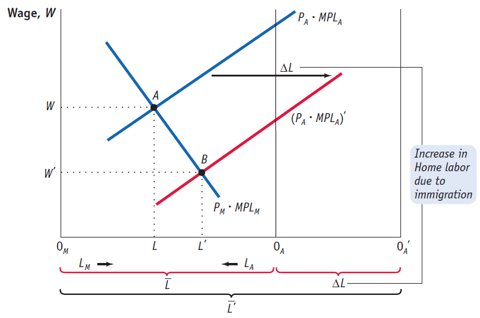
\includegraphics[width = 0.9\textwidth]{tutorial4_heckscher_ohlin2/feenstra5_2.png}
\end{center}

\begin{enumerate}
    \item Migrant labor enters both sectors on equal terms; sectoral L mobility lowers wages equally 
    \item K \& T unchanged; $\bar{L} \uparrow$, MPL $\downarrow$, wage falls
\end{enumerate}

% think here about wage as the price of factor labor: with increasing supply of labor, the price of the the factor falls
% equilibrium is where both sector pay the same wage: no incentive change sector

\end{frame}

\fi


%========================
% MIGRATION SHORT-RUN: QUESTION - OUTPUT & GAINS
%========================

\begin{frame}{Migration (Short Run): What happens to output and factor returns?}

\textbf{Still in the specific-factors model, consider the effects of the immigration-induced labor inflow on output and on the returns to capital and land.}

\vspace{0.3cm}

\begin{enumerate}
    \item What happens to output in each sector, and why?
    \item What happens to $MPK$ and $MPT$, and why?
    \item Who are the winners and losers from immigration?
\end{enumerate}

\end{frame}



\begin{frame}{Migration (Short Run): Effect on PPF}

\begin{center}
\begin{tikzpicture}[scale=0.9]

% === Dimensions ===
\def\width{7}
\def\height{6}

% === Axes ===
% Y-axis (Output of agriculture)
\draw[thick, ->] (0,0) -- (0,\height) 
    node[above, align=center] {Output of \\ agriculture, $Q_A$};

% X-axis (Output of manufacturing)
\draw[thick, ->] (0,0) -- (\width,0) 
    node[right, align=center] {Output of \\ manufacturing, $Q_M$};

\end{tikzpicture}
\end{center}

\end{frame}



%========================
% MIGRATION SHORT-RUN: ANSWER - OUTPUT
%========================

\ifnum\showanswers=1

\begin{frame}{Migration (Short Run): Effect on PPF}

\begin{center}
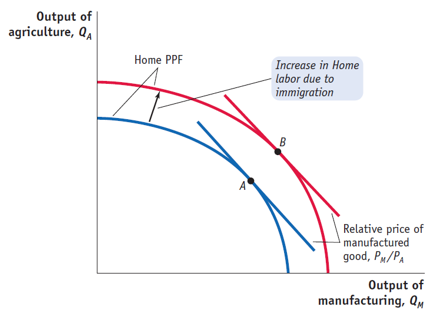
\includegraphics[width = 0.7\textwidth]{tutorial4_heckscher_ohlin2/feenstra5_5.png}
\end{center}

\begin{enumerate}
    \item PPF shifts symmetrically. $Q_M \uparrow$, $Q_A \uparrow$ as ($\uparrow$ L in both sectors)
    \item $MPK \uparrow$ (more L per machine $\Rightarrow$) \& $MPT \uparrow$ (more L per acre)
    \item Winners: K \& T owners (rentals $\uparrow$). Losers: Workers (wage $\downarrow$)
\end{enumerate}
\end{frame}

\fi


%========================
% MIGRATION LONG-RUN: QUESTION
%========================
\begin{frame}{Migration (Long Run): What happens when Home receives immigrants?}

\textbf{Now both L and K are mobile across sectors (shoes and computers). Using the box diagram, explain how the economy absorbs additional labor.}

\vspace{0.2cm}

\textit{Box diagram:} 
\begin{itemize}
    \item bottom axis = total labor $\bar{L}$ 
    \item left axes = total capital $\bar{K}$
    \item Origins: $O_S$ (shoes/labor-intensive), $O_C$ (computers/capital-intensive)
\end{itemize}

\vspace{0.1cm}

\begin{enumerate}
    \item Which sector absorbs the additional labor?
    \item What happens to the capital--labor ratio in each sector?
    \item What happens to wages and rentals?
\end{enumerate}

\end{frame}





\begin{frame}{The Box Diagram: Step 1 — One Sector (Shoes)}

\begin{center}
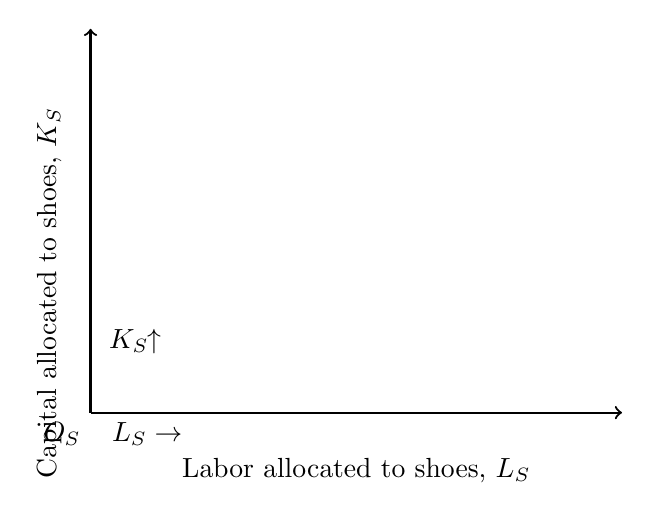
\begin{tikzpicture}[scale=0.75]

% === Dimensions ===
\def\boxW{9}
\def\boxH{6.5}

% === Two axes only ===
% Bottom axis (x)
\draw[thick, ->] (0,0) -- (\boxW,0);
% Left axis (y)
\draw[thick, ->] (0,0) -- (0,\boxH);

% === Origin label ===
\node[below left] at (0,0) {$O_S$};

% === L_S direction ===
\node[below right] at (0.2, 0) {$L_S \rightarrow$};

% === Left axis label (upper portion) ===
\node[left, align=center, rotate=90] at (-0.7, \boxH * 0.82) 
    {Capital allocated to shoes, $K_S$};

% === K_S direction ===
\node[right] at (0.15, 1.2) {$K_S \!\!\uparrow$};

% === Bottom label ===
\node[below] at (\boxW/2, -0.6) 
    {Labor allocated to shoes, $L_S$};

\end{tikzpicture}
\end{center}
\end{frame}

% From origin $O_S$, labor in shoes ($L_S$) is measured \textbf{rightward} and capital in shoes ($K_S$) is measured \textbf{upward}. Any point in this space represents a particular factor allocation — and the slope of a ray from $O_S$ to that point gives the $K_S/L_S$ ratio.

\begin{frame}{The Box Diagram: Step 2 — Both Sectors}

\begin{center}
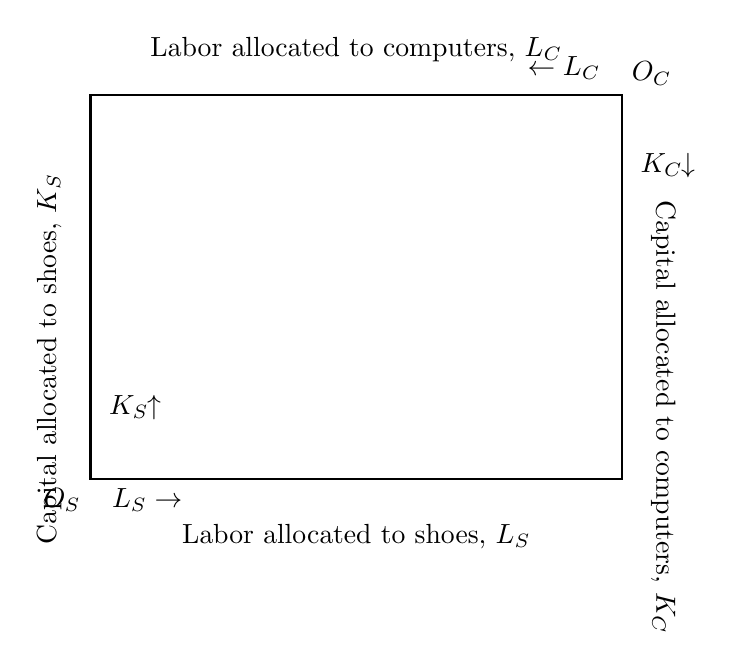
\begin{tikzpicture}[scale=0.75]

% === Dimensions ===
\def\boxW{9}
\def\boxH{6.5}

% === Full box ===
\draw[thick] (0,0) rectangle (\boxW,\boxH);

% === Origin labels ===
\node[below left] at (0,0) {$O_S$};
\node[above right] at (\boxW,\boxH) {$O_C$};

% === Bottom axis: Labor allocated to shoes ===
\node[below right] at (0.2, 0) {$L_S \rightarrow$};
\node[below] at (\boxW/2, -0.6) 
    {Labor allocated to shoes, $L_S$};

% === Left axis: Capital allocated to shoes (upper portion) ===
\node[left, align=center, rotate=90] at (-0.7, \boxH * 0.82) 
    {Capital allocated to shoes, $K_S$};
\node[right] at (0.15, 1.2) {$K_S \!\!\uparrow$};

% === Top axis: Labor allocated to computers ===
\node[above] at (\boxW/2, \boxH + 0.4) 
    {Labor allocated to computers, $L_C$};
\node[above left] at (\boxW - 0.2, \boxH + 0.1) {$\leftarrow L_C$};

% === Right axis: Capital allocated to computers ===
\node[right, align=center, rotate=270] at (\boxW + 0.7, \boxH * 0.75) 
    {Capital allocated to computers, $K_C$};
\node[right] at (\boxW + 0.15, \boxH - 1.2) {$K_C \!\!\downarrow$};

\end{tikzpicture}
\end{center}

\end{frame}

\begin{frame}{The Box Diagram: Step 3 - Migration}

\begin{center}
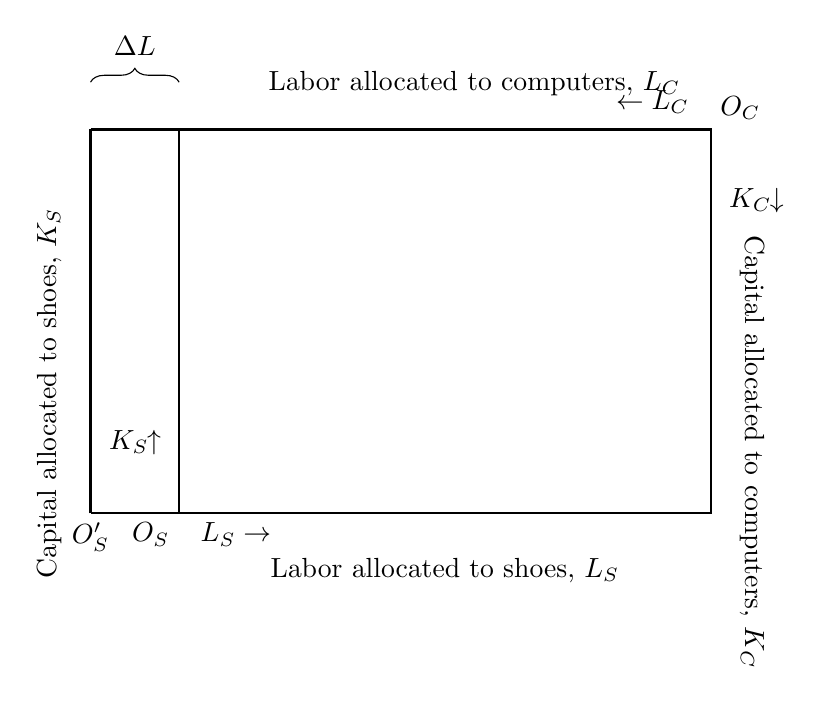
\begin{tikzpicture}[scale=0.75]

% === Dimensions ===
\def\boxW{9}
\def\boxH{6.5}
\def\shift{1.5}

% === Original box ===
\draw[thick] (0,0) rectangle (\boxW,\boxH);

% === Extended portion (post-immigration) ===
\draw[thick] (-\shift,0) -- (0,0);
\draw[thick] (-\shift,\boxH) -- (0,\boxH);
\draw[thick] (-\shift,0) -- (-\shift,\boxH);

% === Origin labels ===
\node[below] at (-\shift,0) {$O'_S$};
\node[below left] at (0,0) {$O_S$};
\node[above right] at (\boxW,\boxH) {$O_C$};

% === Delta L brace (top) ===
\draw[decorate, decoration={brace, amplitude=5pt}] 
    (-\shift,\boxH + 0.8) -- (0,\boxH + 0.8) 
    node[midway, above=6pt] {$\Delta L$};

% === Bottom axis: Labor allocated to shoes ===
\node[below right] at (0.2, 0) {$L_S \rightarrow$};
\node[below] at (\boxW/2, -0.6) 
    {Labor allocated to shoes, $L_S$};

% === Left axis: Capital allocated to shoes (upper portion) ===
\node[left, align=center, rotate=90] at (-\shift - 0.7, \boxH * 0.82) 
    {Capital allocated to shoes, $K_S$};
\node[right] at (-\shift + 0.15, 1.2) {$K_S \!\!\uparrow$};

% === Top axis: Labor allocated to computers ===
\node[above] at (\boxW/2 + 0.5, \boxH + 0.4) 
    {Labor allocated to computers, $L_C$};
\node[above left] at (\boxW - 0.2, \boxH + 0.1) {$\leftarrow L_C$};

% === Right axis: Capital allocated to computers ===
\node[right, align=center, rotate=270] at (\boxW + 0.7, \boxH * 0.75) 
    {Capital allocated to computers, $K_C$};
\node[right] at (\boxW + 0.15, \boxH - 1.2) {$K_C \!\!\downarrow$};

\end{tikzpicture}
\end{center}

\end{frame}


%========================
% MIGRATION LONG-RUN: ANSWER - BOX DIAGRAM
%========================

\ifnum\showanswers=1

\begin{frame}{Migration (Long Run): Box Diagram}


\begin{center}
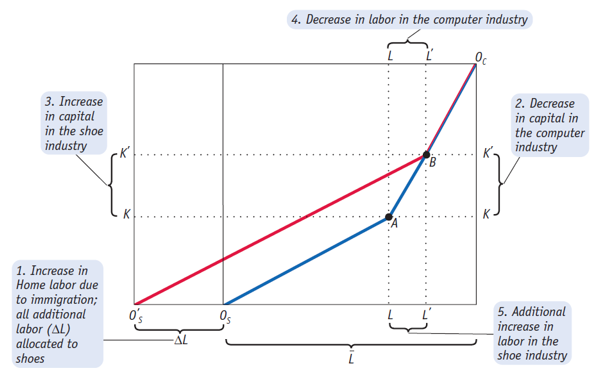
\includegraphics[width = 0.8\textwidth]{tutorial4_heckscher_ohlin2/feenstra5_8.png}
\end{center}

\vspace{0.1cm}

\small
\begin{enumerate}
    \item All additional labor absorbed by \textbf{labor-intensive} sector (shoes) as it is most productively deployed there
    \item Shoes also pulls capital (and extra labor) from computers
    \item $K/L$ ratio \textbf{unchanged} in both sectors $\Rightarrow$ \textbf{wages \& rentals unchanged}
\end{enumerate}
\end{frame}

\fi


%========================
% MIGRATION LONG-RUN: MECHANISM EXPLANATION
%========================

\ifnum\showanswers=1

\begin{frame}{Why do factor prices not change? The mechanism step by step}

\begin{enumerate}
    \item Immigration increases total $L$ (box widens by $\Delta L$)

    \vspace{0.1cm}

    \item The labor-intensive sector (shoes) uses labor most intensively, so it can absorb the extra workers most productively $\Rightarrow$ immigrants enter shoes

    \vspace{0.1cm}

    \item This would raise $L/K$ in shoes, pushing up $MPK$ there $\Rightarrow$ capital moves from computers to shoes

    \vspace{0.1cm}

    \item But capital leaving computers raises $K/L$ there (too few machines per worker) $\Rightarrow$ some labor also leaves computers for shoes

    \vspace{0.1cm}

    \item Reallocation of \textbf{both} factors continues until $K/L$ ratios are restored in \textbf{both} sectors

    \vspace{0.1cm}

    \item With unchanged $K/L$ ratios: $MPL$ and $MPK$ unchanged $\Rightarrow$ $w$ and $r$ unchanged

\end{enumerate}

\vspace{0.3cm}

This is \textbf{factor price insensitivity}: the economy absorbs factor inflows by changing \textit{what} it produces, not \textit{what} it pays.

\end{frame}
\fi


%========================
% RYBCZYNSKI: QUESTION
%========================

\begin{frame}{What happens to output after immigration? (Rybczynski Theorem)}

\textbf{Using the PPF diagram, show how immigration affects the output of each industry in the long run.}

\vspace{0.2cm}

\textit{Axes: x-axis = Output of computers ($Q_C$); y-axis = Output of shoes ($Q_S$).}

\vspace{0.3cm}

\begin{enumerate}
    \item How does the PPF shift?
    \item How does the new production point compare to the short-run result?
\end{enumerate}

\end{frame}


%========================
% RYBCZYNSKI: ANSWER
%========================

\ifnum\showanswers=1

\begin{frame}{Rybczynski Theorem: Immigration}

% PLACEHOLDER: Insert Feenstra Figure 5-9 (PPF shift, Rybczynski)
\begin{center}
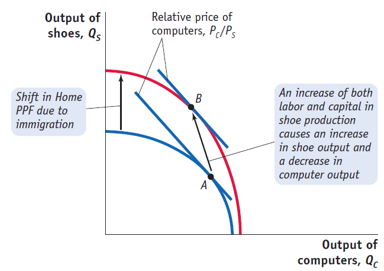
\includegraphics[width = 0.8\textwidth]{tutorial4_heckscher_ohlin2/feenstra5_9.png}
\end{center}


\textbf{Rybczynski Theorem:} An increase in a factor's endowment increases output of the industry using that factor intensively and \textbf{decreases} output of the other industry.

\vspace{0.2cm}

$\Rightarrow$ Shoe output $\uparrow$, computer output $\downarrow$ (contrast short run: both $\uparrow$)

\end{frame}

\fi


%========================
% SECTION 3: FDI
%========================

\begin{frame}

\vspace{2cm}

\centering
{\LARGE \textbf{Section 3}} \\[0.5cm]
{\Large Foreign Direct Investment (Movement of Capital)}

\vfill

\end{frame}


%========================
% FDI SHORT-RUN: QUESTION
%========================

\begin{frame}{FDI (Short Run): What happens when Home receives an inflow of capital?}

\textbf{Using the wage-labor diagram, analyze the effects of an inflow of foreign capital in home.}

\vspace{0.2cm}

\textit{Axes: x-axis = Labor ($L_M$ increasing left to right, $L_A$ increasing right to left); y-axis = Wage ($w$).}

\vspace{0.3cm}

\begin{enumerate}
    \item Which home sector absorbs the foreign capital?
    \item What happens to the sectoral labor allocation \& wages?
    \item What happens to total \& sectoral output?
\end{enumerate}

\end{frame}

%========================
% FDI SHORT-RUN: ANSWER - WAGES & OUTPUT
%========================

\ifnum\showanswers=1

\begin{frame}{FDI (Short Run): Effect on Wages and Output}

\begin{center}
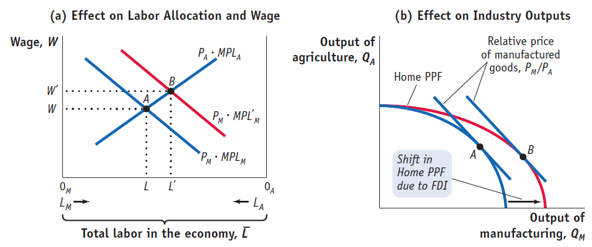
\includegraphics[width = 0.9\textwidth]{tutorial4_heckscher_ohlin2/feenstra5_11.png}
\end{center}

\begin{enumerate}
    \item Capital enters manufacturing (K is specific to manufacturing)
    \item More K in manufacturing $\Rightarrow$ workers have more machines $\Rightarrow$ $MPL_M \uparrow$ $\Rightarrow$ higher wages attract labor from agriculture ($\Rightarrow$ $MPL_K \uparrow$). Wage rises: $W \rightarrow W'$
    \item $Q_M \uparrow$ (more K and more L), $Q_A \downarrow$ (labor leaves agriculture)
\end{enumerate}

\end{frame}

\fi


%========================
% FDI SHORT-RUN: RENTAL ON CAPITAL & WINNERS/LOSERS
%========================

% \ifnum\showanswers=1

% \begin{frame}{FDI (Short Run): What happens to the rental on capital?}

% \begin{center}
% 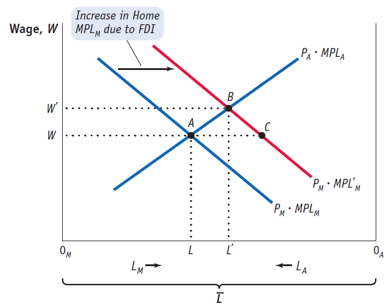
\includegraphics[width = 0.8\textwidth]{tutorial4_heckscher_ohlin2/feenstra5_12.png}
% \end{center}

% \vspace{0.2cm}

% \begin{itemize}
%     \item A $\rightarrow$ C: Extra K at unchanged wage $\Rightarrow$ $K/L$ ratio unchanged $\Rightarrow$ $MPK$ unchanged
%     \item C $\rightarrow$ B: Wage rises, fewer workers per machine $\Rightarrow$ $MPK \downarrow$
%     \item \textbf{Net effect: rental on capital falls}
% \end{itemize}

% \vspace{0.2cm}

% \textit{Intuition: FDI floods manufacturing with capital. Even though workers follow, there are still more machines per worker than before.}

% \vspace{0.2cm}

% \textbf{Winners:} Workers ($w \uparrow$). \textbf{Losers:} Land owners ($L_A \downarrow \Rightarrow MPT \downarrow$) and capital owners ($MPK \downarrow$).

% \end{frame}

% \fi


\ifnum\showanswers=1
\begin{frame}{FDI (Short Run): What happens to wages, the rental on capital, and the rental on land?}

\textbf{FDI increases capital in manufacturing ($K_M \uparrow$, with $L$ fixed).}
\begin{itemize}
    \item More machines per worker in manufacturing $\Rightarrow$ $MPL_M \uparrow$
    \item Manufacturing firms bid up wages to attract labor $\Rightarrow$ $w \uparrow$
    \item Labor moves from agriculture to manufacturing: $L_M \uparrow$, $L_A \downarrow$
\end{itemize}

\vspace{0.2cm}

\textbf{Effect on the rental on land ($R_T$).}
\begin{itemize}
    \item Fewer workers per acre in agriculture $\Rightarrow$ $MPT \downarrow$ $\Rightarrow$ \textbf{$R_T$ falls}
\end{itemize}

\vspace{0.2cm}

\textbf{Effect on the rental on capital ($R_K$).}
\begin{itemize}
    \item Two countervailing effects on $MPK$:
    \begin{itemize}
        \item[$\downarrow$] More capital (diminishing returns): more machines per worker
        \item[$\uparrow$] More labor enters manufacturing: more workers per machine
    \end{itemize}
    \item \textbf{Net effect: $R_K$ falls.} The capital increase is the \textit{initial shock}; the labor inflow is a \textit{partial} response to higher wages. The $K/L$ ratio in manufacturing is higher than before $\Rightarrow$ $MPK \downarrow$.
\end{itemize}

\vspace{0.2cm}

\textbf{Winners:} Workers ($w \uparrow$). \hspace{0.02cm} \textbf{Losers:} Land owners ($R_T \downarrow$) \& capital owners ($R_K \downarrow$).

\end{frame}
\fi


%========================
% FDI LONG-RUN: QUESTION
%========================

\begin{frame}{FDI (Long Run): What happens when Home receives an inflow of capital?}

\textbf{Now both L and K are mobile across sectors. Using the box diagram and PPF, analyze the long-run effects of FDI.}

\vspace{0.3cm}

\begin{enumerate}
    \item Which sector absorbs the additional capital, and why?
    \item What happens to wages and rentals?
    \item What happens to output in each sector?
\end{enumerate}

\end{frame}


%========================
% FDI LONG-RUN: ANSWER
%========================

\ifnum\showanswers=1

\begin{frame}{FDI (Long Run): Box Diagram and Output}

\begin{center}
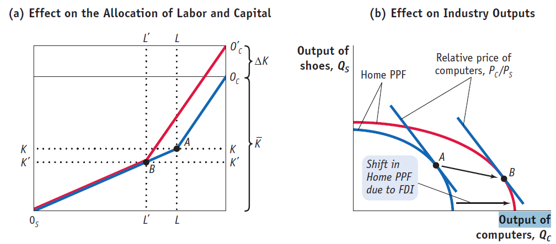
\includegraphics[width = 0.9\textwidth]{tutorial4_heckscher_ohlin2/feenstra5_13.png}
\end{center}

\vspace{0.1cm}

\small
\begin{enumerate}
    \item All additional capital absorbed by the \textbf{capital-intensive} sector (computers) --- because computers use capital most intensively, the extra capital is most productively deployed there (highest $MPK$)
    \item $K/L$ ratios unchanged $\Rightarrow$ \textbf{wages and rentals unchanged} (factor price insensitivity)
    \item Rybczynski: $Q_C \uparrow$, $Q_S \downarrow$ (PPF shifts toward computers)
\end{enumerate}

\end{frame}

\fi


%========================
% SECTION 4: EMPIRICAL EVIDENCE
%========================

\begin{frame}

\vspace{2cm}

\centering
{\LARGE \textbf{Section 4}} \\[0.5cm]
{\Large Empirical Evidence}

\vfill

\end{frame}


%========================
% EMPIRICS: QUESTION
%========================

\begin{frame}{Do real-world episodes support the short-run or long-run predictions?}

\textbf{Consider two large-scale immigration episodes:}

\vspace{0.3cm}

\begin{enumerate}
    \item \textbf{Mariel Boatlift (1980):} 125,000 Cuban refugees arrived in Miami, increasing the labor force by $\sim$7\%.

    \vspace{0.2cm}

    \item \textbf{Russian immigration to Israel (early 1990s):} $\sim$700,000 immigrants, increasing the population by $\sim$12\%.
\end{enumerate}

\vspace{0.3cm}

Did wages fall (short-run prediction) or remain stable (long-run prediction)?

\end{frame}


%========================
% EMPIRICS: ANSWER - MIGRATION
%========================

\ifnum\showanswers=1

\begin{frame}{Evidence: Mariel Boatlift and Russian Immigration to Israel}

\textbf{Mariel Boatlift (Card, 1990):}
\begin{itemize}
    \item Virtually no effect on Miami wages despite 7\% labor force increase
    \item Apparel industry (labor-intensive) expanded relative to comparison cities; skill-intensive industries contracted
    \item Consistent with \textbf{Rybczynski adjustment}
\end{itemize}

\vspace{0.3cm}

\textbf{Russian immigration to Israel (Gandal, Hanson \& Slaughter, 2004):}
\begin{itemize}
    \item Israel absorbed 12\% population increase through export expansion in high-tech (matching immigrants' skills)
    \item Output adjustment, not wage collapse
\end{itemize}

\vspace{0.3cm}

$\Rightarrow$ Open economies can absorb immigrants through \textbf{industry composition changes}, supporting the long-run model.

\end{frame}

\fi


%========================
% EMPIRICS: QUESTION - FDI
%========================

\begin{frame}{Does FDI lower the return on capital, or can the economy adjust?}

\textbf{Singapore} has attracted massive FDI since the 1970s (4th largest stock of foreign capital in the world).

\vspace{0.3cm}

What does the evidence suggest about the effect on rentals and wages?

\end{frame}


%========================
% EMPIRICS: ANSWER - FDI (Singapore)
%========================

\ifnum\showanswers=1

\begin{frame}{Evidence: FDI in Singapore}

\textbf{Two measurement approaches yield different results:}

\vspace{0.2cm}

\begin{center}
\small
\begin{tabular}{lcc}
\toprule
\textbf{Method} & \textbf{Real rental} & \textbf{Real wage} \\
\midrule
Production function & $-3.4\%$/yr & $+1.6\%$/yr \\
(Young, 1995) & & \\
\midrule
Market-based rental & $\approx 0\%$/yr & $+2.7$ to $3.6\%$/yr \\
(Hsieh, 2002) & & \\
\bottomrule
\end{tabular}
\end{center}

\vspace{0.3cm}

\begin{itemize}
    \item Method A $\Rightarrow$ consistent with \textbf{short-run} model (diminishing returns to K)
    \item Method B $\Rightarrow$ consistent with \textbf{long-run} model (industry adjustment)
\end{itemize}

\vspace{0.2cm}

\textit{Reality likely between the two: Singapore adjusted industry composition (expanding electronics), but the speed of capital inflows partially depressed rentals.}

\end{frame}

\fi


%========================
% SECTION 5: CONCLUSION
%========================

\begin{frame}

\vspace{2cm}

\centering
{\LARGE \textbf{Conclusion}}

\vfill

\end{frame}


%========================
% SUMMARY TABLE
%========================

\begin{frame}{Summary: Short-Run vs. Long-Run Effects}

\begin{center}
\small
\begin{tabular}{lcccc}
\toprule
& \multicolumn{2}{c}{\textbf{Migration ($\uparrow L$)}} & \multicolumn{2}{c}{\textbf{FDI ($\uparrow K$)}} \\
\cmidrule(lr){2-3} \cmidrule(lr){4-5}
& \textbf{SR} & \textbf{LR} & \textbf{SR} & \textbf{LR} \\
\midrule
Wage & $\downarrow$ & unchanged & $\uparrow$ & unchanged \\
Rental on K & $\uparrow$ & unchanged & $\downarrow$ & unchanged \\
Rental on T & $\uparrow$ & --- & $\downarrow$ & --- \\
\midrule
$Q$ (L-intensive) & $\uparrow$ & $\uparrow$ & $\downarrow$ & $\downarrow$ \\
$Q$ (K-intensive) & $\uparrow$ & $\downarrow$ & $\uparrow$ & $\uparrow$ \\
\bottomrule
\end{tabular}
\end{center}

\vspace{0.3cm}

\textbf{Key contrast:} In the short run, both sectors expand; in the long run, only the sector intensive in the inflowing factor expands (Rybczynski), and factor prices are unchanged (factor price insensitivity).

\end{frame}


%========================
% KEY TAKEAWAYS
%========================

\begin{frame}{Key Takeaways}

\begin{enumerate}
    \item In the \textbf{short run}, factor inflows change factor prices --- immigration lowers wages, FDI lowers rentals

    \vspace{0.2cm}

    \item In the \textbf{long run}, factor inflows are absorbed through changes in industry composition (\textbf{Rybczynski}), leaving factor prices unchanged (\textbf{factor price insensitivity})

    \vspace{0.2cm}

    \item Empirical evidence (Mariel Boatlift, Israel, Singapore) suggests economies can adjust through output changes when open to trade

    \vspace{0.2cm}

    \item Trade, migration, and FDI are \textbf{substitutes} for achieving factor price convergence
\end{enumerate}

\vspace{0.3cm}

\textit{After reading week: The Standard Trade Model.}

\end{frame}



\fi



\ifnum\showanswers=0
\subsection{HO Migration + Capital w/o Answers}

%========================
% TITLE SLIDE
%========================

\begin{frame}

\vspace{1.5cm}

\centering
{\Large \textbf{Tutorial 4: The Heckscher-Ohlin Model \\ (Part 2)}} \\[0.5cm]
{\large Movement of Labor \& Capital between Countries} \\[1.0cm]

{\small 7QQMM209: International Economics} \\[0.3cm]
{\small King's College London}

\vfill

\end{frame}

%========================
% AGENDA
%========================

\begin{frame}{Agenda}

\begin{enumerate}
    \item \textbf{Intro: Specific Factors vs. Factor Proportion Model} \\~\\

    \item \textbf{Migration}
    \begin{itemize}
        \item Short-run effects (Specific Factors)
        \item Long-run effects (Heckscher-Ohlin)
    \end{itemize}

    \vspace{0.3cm}

    \item \textbf{Foreign Direct Investment (FDI)}
    \begin{itemize}
        \item Short-run effects (Specific Factors)
        \item Long-run effects (Heckscher-Ohlin)
    \end{itemize}

    \vspace{0.3cm}

    \item \textbf{Empirical Evidence}
\end{enumerate}

\end{frame}

%========================
% REFERENCES
%========================

\begin{frame}{References: Textbook Chapters}

\textbf{Primary readings:}
\begin{itemize}
    \item \textbf{Feenstra \& Taylor:} Chapter 5 --- Movement of Labor and Capital between Countries \\~\\
    \item \textbf{Feenstra \& Taylor:} Chapter 4 --- Trade and Resources: The Heckscher-Ohlin Model (recap)
\end{itemize}

\end{frame}

%========================
% KEY CONCEPTS
%========================

\begin{frame}{Key Concepts for This Tutorial}

\begin{itemize}
    \item \textbf{Rybczynski Theorem}

    \vspace{0.3cm}

    \item \textbf{Factor Price Insensitivity}

    \vspace{0.3cm}

    \item \textbf{Box Diagram} (allocation of L and K across industries)

\end{itemize}

\end{frame}


%========================
% SECTION 1: TRANSITION & RECAP
%========================

\begin{frame}

\vspace{2cm}

\centering
{\LARGE \textbf{Section 1}} \\[0.5cm]
{\Large Recap: Specific Factors vs. Factor Proportion Model (HO)}

\vfill

\end{frame}

%========================
% TRANSITION
%========================

\begin{frame}{Three Ways to Achieve Factor Price Convergence}

\begin{itemize}
    \item \textbf{Trade} = Mobility of goods
    \item \textbf{Migration} = Mobility of labor
    \item \textbf{FDI} = Mobility of capital
\end{itemize}

\vspace{0.5cm}

\textbf{Last week:} Long-run effects of \textbf{trade} in the HO model.

\vspace{0.2cm}

\textbf{This week:} Short-run \textbf{and} long-run effects of \textbf{migration} and \textbf{FDI}.

\end{frame}


%========================
% A: Model Comparison
%========================

\ifnum\showanswers=0

\begin{frame}{Specific Factors (Short Run) vs. Factor Proportion (Long Run)}

\begin{columns}[T]
\begin{column}{0.48\textwidth}
\textbf{Specific Factors (SR)}
\begin{itemize}
    \item 3 factors: L, K, T
    \item K and T sector-specific
    \item Labor mobile across sectors
    \item Diminishing returns $\Rightarrow$ factor inflows change factor prices
\end{itemize}
\end{column}

\begin{column}{0.48\textwidth}
\textbf{Factor Proportion / HO (LR)}
\begin{itemize}
    \item 2 factors: L, K
    \item Both mobile across sectors
    \item Economy absorbs inflows via output adjustment
    \item Factor prices unchanged
\end{itemize}
\end{column}
\end{columns}

\vspace{0.5cm}

\textbf{Key:} In the short run, factor inflows create winners and losers. In the long run, industry composition adjusts instead.

\end{frame}

\fi

%========================
% SECTION 2: MIGRATION
%========================

\begin{frame}

\vspace{2cm}

\centering
{\LARGE \textbf{Section 2}} \\[0.5cm]
{\Large Migration (Movement of Labor)}

\vfill

\end{frame}


%========================
% MIGRATION SHORT-RUN: QUESTION
%========================

\begin{frame}{Migration (Short Run): What happens when Home receives immigrants?}

\textbf{Using the specific-factors labor allocation diagram, analyze the effect of an inflow of immigrants ($\Delta L$) on Home.}

\vspace{0.2cm}

\textit{Axes: x-axis = Labor ($L_M$ increasing left to right, $L_A$ increasing right to left); y-axis = Wage ($w$).}

\vspace{0.3cm}

\begin{enumerate}
    \item How is the additional labor allocated, \& why?
    \item What happens to K, T, $\bar{L}$ \& MPL?
    \item What happens to wages?
\end{enumerate}

\end{frame}


%========================
% MIGRATION SHORT-RUN: ANSWER - WAGES
%========================

\ifnum\showanswers=0

\begin{frame}{Migration (Short Run): Effect on Wages and Output}

\begin{center}
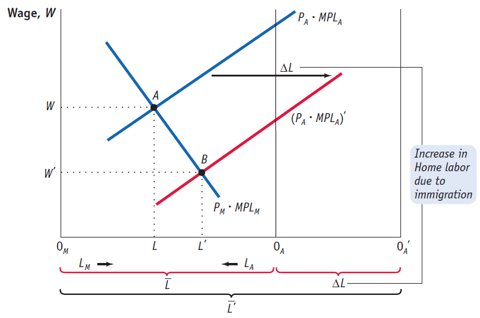
\includegraphics[width = 0.9\textwidth]{tutorial4_heckscher_ohlin2/feenstra5_2.png}
\end{center}

\begin{enumerate}
    \item Migrant labor enters both sectors on equal terms; sectoral L mobility lowers wages equally 
    \item K \& T unchanged; $\bar{L} \uparrow$, MPL $\downarrow$, wage falls
\end{enumerate}

% think here about wage as the price of factor labor: with increasing supply of labor, the price of the the factor falls
% equilibrium is where both sector pay the same wage: no incentive change sector

\end{frame}

\fi


%========================
% MIGRATION SHORT-RUN: QUESTION - OUTPUT & GAINS
%========================

\begin{frame}{Migration (Short Run): What happens to output and factor returns?}

\textbf{Still in the specific-factors model, consider the effects of the immigration-induced labor inflow on output and on the returns to capital and land.}

\vspace{0.3cm}

\begin{enumerate}
    \item What happens to output in each sector, and why?
    \item What happens to $MPK$ and $MPT$, and why?
    \item Who are the winners and losers from immigration?
\end{enumerate}

\end{frame}


%========================
% MIGRATION SHORT-RUN: ANSWER - OUTPUT
%========================

\ifnum\showanswers=0

\begin{frame}{Migration (Short Run): Effect on PPF}

\begin{center}
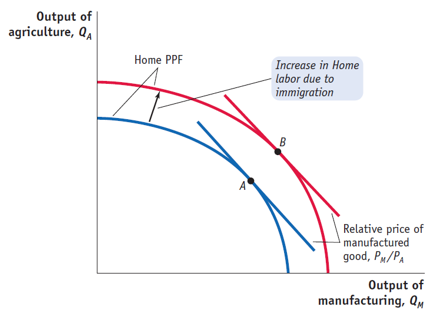
\includegraphics[width = 0.7\textwidth]{tutorial4_heckscher_ohlin2/feenstra5_5.png}
\end{center}

\begin{enumerate}
    \item PPF shifts symmetrically. $Q_M \uparrow$, $Q_A \uparrow$ as ($\uparrow$ L in both sectors)
    \item $MPK \uparrow$ (more L per machine $\Rightarrow$) \& $MPT \uparrow$ (more L per acre)
    \item Winners: K \& T owners (rentals $\uparrow$). Losers: Workers (wage $\downarrow$)
\end{enumerate}
\end{frame}

\fi


%========================
% MIGRATION LONG-RUN: QUESTION
%========================

\begin{frame}{Migration (Long Run): What happens when Home receives immigrants?}

\textbf{Now both L and K are mobile across sectors. Using the box diagram, explain how the economy absorbs additional labor.}

\vspace{0.2cm}

\textit{Box diagram: bottom axis = total labor $\bar{L}$; left axis = total capital $\bar{K}$. Origins: $O_S$ (shoes/labor-intensive), $O_C$ (computers/capital-intensive).}

\vspace{0.3cm}

\begin{enumerate}
    \item Which sector absorbs the additional labor?
    \item What happens to the capital--labor ratio in each sector?
    \item What happens to wages and rentals?
\end{enumerate}

\end{frame}


%========================
% MIGRATION LONG-RUN: ANSWER - BOX DIAGRAM
%========================

\ifnum\showanswers=0

\begin{frame}{Migration (Long Run): Box Diagram}


\begin{center}
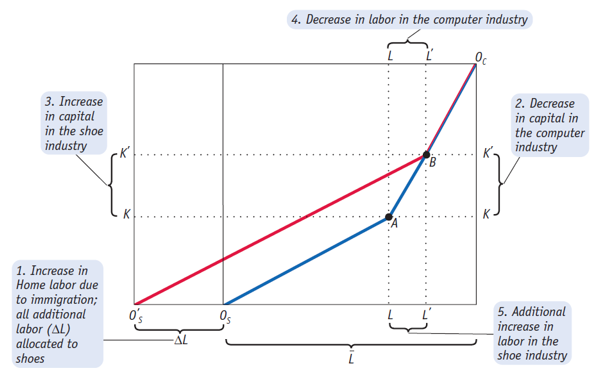
\includegraphics[width = 0.8\textwidth]{tutorial4_heckscher_ohlin2/feenstra5_8.png}
\end{center}

\vspace{0.1cm}

\small
\begin{enumerate}
    \item All additional labor absorbed by \textbf{labor-intensive} sector (shoes) as it is most productively deployed there
    \item Shoes also pulls capital (and extra labor) from computers
    \item $K/L$ ratio \textbf{unchanged} in both sectors $\Rightarrow$ \textbf{wages \& rentals unchanged}
\end{enumerate}
\end{frame}

\fi


%========================
% MIGRATION LONG-RUN: MECHANISM EXPLANATION
%========================

\ifnum\showanswers=0

\begin{frame}{Why do factor prices not change? The mechanism step by step}

\begin{enumerate}
    \item Immigration increases total $L$ (box widens by $\Delta L$)

    \vspace{0.1cm}

    \item The labor-intensive sector (shoes) uses labor most intensively, so it can absorb the extra workers most productively $\Rightarrow$ immigrants enter shoes

    \vspace{0.1cm}

    \item This would raise $L/K$ in shoes, pushing up $MPK$ there $\Rightarrow$ capital moves from computers to shoes

    \vspace{0.1cm}

    \item Reallocation continues until $K/L$ ratios are restored in \textbf{both} sectors

    \vspace{0.1cm}

    \item With unchanged $K/L$ ratios: $MPL$ and $MPK$ unchanged $\Rightarrow$ $w$ and $r$ unchanged

\end{enumerate}

\vspace{0.3cm}

This is \textbf{factor price insensitivity}: the economy absorbs factor inflows by changing \textit{what} it produces, not \textit{what} it pays.

\end{frame}

\fi


%========================
% RYBCZYNSKI: QUESTION
%========================

\begin{frame}{What happens to output after immigration? (Rybczynski Theorem)}

\textbf{Using the PPF diagram, show how immigration affects the output of each industry in the long run.}

\vspace{0.2cm}

\textit{Axes: x-axis = Output of computers ($Q_C$); y-axis = Output of shoes ($Q_S$).}

\vspace{0.3cm}

\begin{enumerate}
    \item How does the PPF shift?
    \item How does the new production point compare to the short-run result?
\end{enumerate}

\end{frame}


%========================
% RYBCZYNSKI: ANSWER
%========================

\ifnum\showanswers=0

\begin{frame}{Rybczynski Theorem: Immigration}

% PLACEHOLDER: Insert Feenstra Figure 5-9 (PPF shift, Rybczynski)
\begin{center}
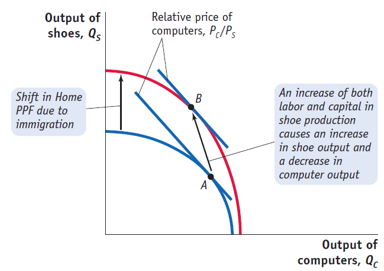
\includegraphics[width = 0.8\textwidth]{tutorial4_heckscher_ohlin2/feenstra5_9.png}
\end{center}


\textbf{Rybczynski Theorem:} An increase in a factor's endowment increases output of the industry using that factor intensively and \textbf{decreases} output of the other industry.

\vspace{0.2cm}

$\Rightarrow$ Shoe output $\uparrow$, computer output $\downarrow$ (contrast short run: both $\uparrow$)

\end{frame}

\fi


%========================
% SECTION 3: FDI
%========================

\begin{frame}

\vspace{2cm}

\centering
{\LARGE \textbf{Section 3}} \\[0.5cm]
{\Large Foreign Direct Investment (Movement of Capital)}

\vfill

\end{frame}


%========================
% FDI SHORT-RUN: QUESTION
%========================

\begin{frame}{FDI (Short Run): What happens when Home receives an inflow of capital?}

\textbf{Using the wage-labor diagram, analyze the effects of an inflow of foreign capital in home.}

\vspace{0.2cm}

\textit{Axes: x-axis = Labor ($L_M$ increasing left to right, $L_A$ increasing right to left); y-axis = Wage ($w$).}

\vspace{0.3cm}

\begin{enumerate}
    \item Which home sector absorbs the foreign capital?
    \item What happens to the sectoral labor allocation \& wages?
    \item What happens to total \& sectoral output?
\end{enumerate}

\end{frame}

%========================
% FDI SHORT-RUN: ANSWER - WAGES & OUTPUT
%========================

\ifnum\showanswers=0

\begin{frame}{FDI (Short Run): Effect on Wages and Output}

\begin{center}
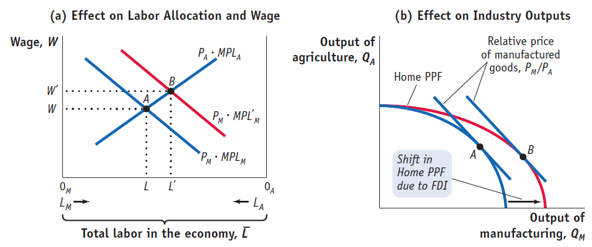
\includegraphics[width = 0.9\textwidth]{tutorial4_heckscher_ohlin2/feenstra5_11.png}
\end{center}

\begin{enumerate}
    \item Capital enters manufacturing (K is specific to manufacturing)
    \item More K in manufacturing $\Rightarrow$ workers have more machines $\Rightarrow$ $MPL_M \uparrow$ $\Rightarrow$ higher wages attract labor from agriculture ($\Rightarrow$ $MPL_K \uparrow$). Wage rises: $W \rightarrow W'$
    \item $Q_M \uparrow$ (more K and more L), $Q_A \downarrow$ (labor leaves agriculture)
\end{enumerate}

\end{frame}

\fi


%========================
% FDI SHORT-RUN: RENTAL ON CAPITAL & WINNERS/LOSERS
%========================

% \ifnum\showanswers=1

% \begin{frame}{FDI (Short Run): What happens to the rental on capital?}

% \begin{center}
% 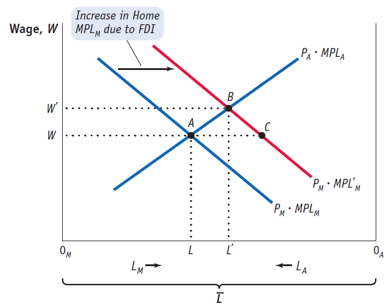
\includegraphics[width = 0.8\textwidth]{tutorial4_heckscher_ohlin2/feenstra5_12.png}
% \end{center}

% \vspace{0.2cm}

% \begin{itemize}
%     \item A $\rightarrow$ C: Extra K at unchanged wage $\Rightarrow$ $K/L$ ratio unchanged $\Rightarrow$ $MPK$ unchanged
%     \item C $\rightarrow$ B: Wage rises, fewer workers per machine $\Rightarrow$ $MPK \downarrow$
%     \item \textbf{Net effect: rental on capital falls}
% \end{itemize}

% \vspace{0.2cm}

% \textit{Intuition: FDI floods manufacturing with capital. Even though workers follow, there are still more machines per worker than before.}

% \vspace{0.2cm}

% \textbf{Winners:} Workers ($w \uparrow$). \textbf{Losers:} Land owners ($L_A \downarrow \Rightarrow MPT \downarrow$) and capital owners ($MPK \downarrow$).

% \end{frame}

% \fi


\ifnum\showanswers=0
\begin{frame}{FDI (Short Run): What happens to wages, the rental on capital, and the rental on land?}

\textbf{FDI increases capital in manufacturing ($K_M \uparrow$, with $L$ fixed).}
\begin{itemize}
    \item More machines per worker in manufacturing $\Rightarrow$ each worker is more productive $\Rightarrow$ $MPL_M \uparrow$
    \item Manufacturing firms bid up wages to attract labor $\Rightarrow$ $w \uparrow$
    \item Labor moves from agriculture to manufacturing: $L_M \uparrow$, $L_A \downarrow$
\end{itemize}

\vspace{0.2cm}

\textbf{Effect on the rental on land ($R_T$).}
\begin{itemize}
    \item Fewer workers per acre in agriculture $\Rightarrow$ $MPT \downarrow$ $\Rightarrow$ \textbf{$R_T$ falls}
\end{itemize}

\vspace{0.2cm}

\textbf{Effect on the rental on capital ($R_K$).}
\begin{itemize}
    \item Two countervailing effects on $MPK$:
    \begin{itemize}
        \item[$\downarrow$] More capital (diminishing returns): more machines compete for workers
        \item[$\uparrow$] More labor enters manufacturing: more workers per machine
    \end{itemize}
    \item \textbf{Net effect: $R_K$ falls.} The capital increase is the \textit{initial shock}; the labor inflow is only a \textit{partial} response to higher wages (agriculture retains some workers). So the $K/L$ ratio in manufacturing is still higher than before $\Rightarrow$ $MPK \downarrow$.
\end{itemize}

\vspace{0.2cm}

\textbf{Winners:} Workers ($w \uparrow$). \quad \textbf{Losers:} Land owners ($R_T \downarrow$) and capital owners ($R_K \downarrow$).

\end{frame}
\fi


%========================
% FDI LONG-RUN: QUESTION
%========================

\begin{frame}{FDI (Long Run): What happens when Home receives an inflow of capital?}

\textbf{Now both L and K are mobile across sectors. Using the box diagram and PPF, analyze the long-run effects of FDI.}

\vspace{0.3cm}

\begin{enumerate}
    \item Which sector absorbs the additional capital, and why?
    \item What happens to wages and rentals?
    \item What happens to output in each sector?
\end{enumerate}

\end{frame}


%========================
% FDI LONG-RUN: ANSWER
%========================

\ifnum\showanswers=0

\begin{frame}{FDI (Long Run): Box Diagram and Output}

\begin{center}
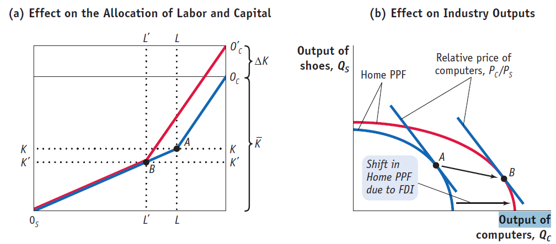
\includegraphics[width = 0.9\textwidth]{tutorial4_heckscher_ohlin2/feenstra5_13.png}
\end{center}

\vspace{0.1cm}

\small
\begin{enumerate}
    \item All additional capital absorbed by the \textbf{capital-intensive} sector (computers) --- because computers use capital most intensively, the extra capital is most productively deployed there (highest $MPK$)
    \item $K/L$ ratios unchanged $\Rightarrow$ \textbf{wages and rentals unchanged} (factor price insensitivity)
    \item Rybczynski: $Q_C \uparrow$, $Q_S \downarrow$ (PPF shifts toward computers)
\end{enumerate}

\end{frame}

\fi


%========================
% SECTION 4: EMPIRICAL EVIDENCE
%========================

\begin{frame}

\vspace{2cm}

\centering
{\LARGE \textbf{Section 4}} \\[0.5cm]
{\Large Empirical Evidence}

\vfill

\end{frame}


%========================
% EMPIRICS: QUESTION
%========================

\begin{frame}{Do real-world episodes support the short-run or long-run predictions?}

\textbf{Consider two large-scale immigration episodes:}

\vspace{0.3cm}

\begin{enumerate}
    \item \textbf{Mariel Boatlift (1980):} 125,000 Cuban refugees arrived in Miami, increasing the labor force by $\sim$7\%.

    \vspace{0.2cm}

    \item \textbf{Russian immigration to Israel (early 1990s):} $\sim$700,000 immigrants, increasing the population by $\sim$12\%.
\end{enumerate}

\vspace{0.3cm}

Did wages fall (short-run prediction) or remain stable (long-run prediction)?

\end{frame}


%========================
% EMPIRICS: ANSWER - MIGRATION
%========================

\ifnum\showanswers=0

\begin{frame}{Evidence: Mariel Boatlift and Russian Immigration to Israel}

\textbf{Mariel Boatlift (Card, 1990):}
\begin{itemize}
    \item Virtually no effect on Miami wages despite 7\% labor force increase
    \item Apparel industry (labor-intensive) expanded relative to comparison cities; skill-intensive industries contracted
    \item Consistent with \textbf{Rybczynski adjustment}
\end{itemize}

\vspace{0.3cm}

\textbf{Russian immigration to Israel (Gandal, Hanson \& Slaughter, 2004):}
\begin{itemize}
    \item Israel absorbed 12\% population increase through export expansion in high-tech (matching immigrants' skills)
    \item Output adjustment, not wage collapse
\end{itemize}

\vspace{0.3cm}

$\Rightarrow$ Open economies can absorb immigrants through \textbf{industry composition changes}, supporting the long-run model.

\end{frame}

\fi


%========================
% EMPIRICS: QUESTION - FDI
%========================

\begin{frame}{Does FDI lower the return on capital, or can the economy adjust?}

\textbf{Singapore} has attracted massive FDI since the 1970s (4th largest stock of foreign capital in the world).

\vspace{0.3cm}

What does the evidence suggest about the effect on rentals and wages?

\end{frame}


%========================
% EMPIRICS: ANSWER - FDI (Singapore)
%========================

\ifnum\showanswers=0

\begin{frame}{Evidence: FDI in Singapore}

\textbf{Two measurement approaches yield different results:}

\vspace{0.2cm}

\begin{center}
\small
\begin{tabular}{lcc}
\toprule
\textbf{Method} & \textbf{Real rental} & \textbf{Real wage} \\
\midrule
Production function & $-3.4\%$/yr & $+1.6\%$/yr \\
(Young, 1995) & & \\
\midrule
Market-based rental & $\approx 0\%$/yr & $+2.7$ to $3.6\%$/yr \\
(Hsieh, 2002) & & \\
\bottomrule
\end{tabular}
\end{center}

\vspace{0.3cm}

\begin{itemize}
    \item Method A $\Rightarrow$ consistent with \textbf{short-run} model (diminishing returns to K)
    \item Method B $\Rightarrow$ consistent with \textbf{long-run} model (industry adjustment)
\end{itemize}

\vspace{0.2cm}

\textit{Reality likely between the two: Singapore adjusted industry composition (expanding electronics), but the speed of capital inflows partially depressed rentals.}

\end{frame}

\fi


%========================
% SECTION 5: CONCLUSION
%========================

\begin{frame}

\vspace{2cm}

\centering
{\LARGE \textbf{Conclusion}}

\vfill

\end{frame}


%========================
% SUMMARY TABLE
%========================

\begin{frame}{Summary: Short-Run vs. Long-Run Effects}

\begin{center}
\small
\begin{tabular}{lcccc}
\toprule
& \multicolumn{2}{c}{\textbf{Migration ($\uparrow L$)}} & \multicolumn{2}{c}{\textbf{FDI ($\uparrow K$)}} \\
\cmidrule(lr){2-3} \cmidrule(lr){4-5}
& \textbf{SR} & \textbf{LR} & \textbf{SR} & \textbf{LR} \\
\midrule
Wage & $\downarrow$ & unchanged & $\uparrow$ & unchanged \\
Rental on K & $\uparrow$ & unchanged & $\downarrow$ & unchanged \\
Rental on T & $\uparrow$ & --- & $\downarrow$ & --- \\
\midrule
$Q$ (L-intensive) & $\uparrow$ & $\uparrow$ & $\downarrow$ & $\downarrow$ \\
$Q$ (K-intensive) & $\uparrow$ & $\downarrow$ & $\uparrow$ & $\uparrow$ \\
\bottomrule
\end{tabular}
\end{center}

\vspace{0.3cm}

\textbf{Key contrast:} In the short run, both sectors expand; in the long run, only the sector intensive in the inflowing factor expands (Rybczynski), and factor prices are unchanged (factor price insensitivity).

\end{frame}


%========================
% KEY TAKEAWAYS
%========================

\begin{frame}{Key Takeaways}

\begin{enumerate}
    \item In the \textbf{short run}, factor inflows change factor prices --- immigration lowers wages, FDI lowers rentals

    \vspace{0.2cm}

    \item In the \textbf{long run}, factor inflows are absorbed through changes in industry composition (\textbf{Rybczynski}), leaving factor prices unchanged (\textbf{factor price insensitivity})

    \vspace{0.2cm}

    \item Empirical evidence (Mariel Boatlift, Israel, Singapore) suggests economies can adjust through output changes when open to trade

    \vspace{0.2cm}

    \item Trade, migration, and FDI are \textbf{substitutes} for achieving factor price convergence
\end{enumerate}

\vspace{0.3cm}

\textit{After reading week: The Standard Trade Model.}

\end{frame}



\fi



\end{document}